%% Anonymised manuscript for double-anonymised review (Information Processing & Management).
%% Author details, acknowledgements and declarations that identify the author are in title_page.tex.
%% Every number in the text is written as \ev{ID}; IDs are the claim IDs of records/evidence-ledger.csv.
\documentclass[a4paper,fleqn]{cas-sc}

\usepackage[authoryear]{natbib}
\usepackage{booktabs}
\usepackage{amsmath}
\usepackage{graphicx}
\usepackage{xcolor}
\usepackage[T1]{fontenc}
\usepackage{mathptmx}
\usepackage[scaled=0.92]{helvet}
\usepackage{courier}
\usepackage[expansion=false]{microtype}
\input{glyphtounicode}
\pdfgentounicode=1
\usepackage{textcomp}
% Generated by manuscript_ipm/tools/make_ledger.py from the committed analysis file. Do not edit by hand.
\makeatletter
\newcommand{\ev}[1]{\ifcsname ev@#1\endcsname\csname ev@#1\endcsname\else\errmessage{Unknown evidence id #1}\fi}
\expandafter\def\csname ev@HIT.nq.R0\endcsname{0.363}
\expandafter\def\csname ev@HIT.nq.R0.ci\endcsname{[0.343, 0.383]}
\expandafter\def\csname ev@HIT.nq.R1\endcsname{0.664}
\expandafter\def\csname ev@HIT.nq.R1.ci\endcsname{[0.645, 0.683]}
\expandafter\def\csname ev@HIT.nq.R2\endcsname{0.729}
\expandafter\def\csname ev@HIT.nq.R2.ci\endcsname{[0.710, 0.747]}
\expandafter\def\csname ev@HIT.nq.R3\endcsname{0.770}
\expandafter\def\csname ev@HIT.nq.R3.ci\endcsname{[0.753, 0.788]}
\expandafter\def\csname ev@HIT.nq.R4\endcsname{0.796}
\expandafter\def\csname ev@HIT.nq.R4.ci\endcsname{[0.779, 0.812]}
\expandafter\def\csname ev@HIT.nq.R5\endcsname{0.816}
\expandafter\def\csname ev@HIT.nq.R5.ci\endcsname{[0.800, 0.832]}
\expandafter\def\csname ev@HIT.nq.R6\endcsname{0.744}
\expandafter\def\csname ev@HIT.nq.R6.ci\endcsname{[0.726, 0.762]}
\expandafter\def\csname ev@EM.qnq.R0\endcsname{0.360}
\expandafter\def\csname ev@EM.qnq.R0.ci\endcsname{[0.340, 0.380]}
\expandafter\def\csname ev@F1.qnq.R0\endcsname{0.463}
\expandafter\def\csname ev@AC.qnq.R0\endcsname{0.427}
\expandafter\def\csname ev@EM.qnq.R1\endcsname{0.471}
\expandafter\def\csname ev@EM.qnq.R1.ci\endcsname{[0.451, 0.492]}
\expandafter\def\csname ev@F1.qnq.R1\endcsname{0.591}
\expandafter\def\csname ev@AC.qnq.R1\endcsname{0.564}
\expandafter\def\csname ev@EM.qnq.R2\endcsname{0.484}
\expandafter\def\csname ev@EM.qnq.R2.ci\endcsname{[0.463, 0.505]}
\expandafter\def\csname ev@F1.qnq.R2\endcsname{0.608}
\expandafter\def\csname ev@AC.qnq.R2\endcsname{0.581}
\expandafter\def\csname ev@EM.qnq.R3\endcsname{0.493}
\expandafter\def\csname ev@EM.qnq.R3.ci\endcsname{[0.473, 0.513]}
\expandafter\def\csname ev@F1.qnq.R3\endcsname{0.619}
\expandafter\def\csname ev@AC.qnq.R3\endcsname{0.600}
\expandafter\def\csname ev@EM.qnq.R4\endcsname{0.503}
\expandafter\def\csname ev@EM.qnq.R4.ci\endcsname{[0.482, 0.524]}
\expandafter\def\csname ev@F1.qnq.R4\endcsname{0.627}
\expandafter\def\csname ev@AC.qnq.R4\endcsname{0.608}
\expandafter\def\csname ev@EM.qnq.R5\endcsname{0.510}
\expandafter\def\csname ev@EM.qnq.R5.ci\endcsname{[0.489, 0.530]}
\expandafter\def\csname ev@F1.qnq.R5\endcsname{0.636}
\expandafter\def\csname ev@AC.qnq.R5\endcsname{0.619}
\expandafter\def\csname ev@EM.qnq.R6\endcsname{0.492}
\expandafter\def\csname ev@EM.qnq.R6.ci\endcsname{[0.471, 0.512]}
\expandafter\def\csname ev@F1.qnq.R6\endcsname{0.612}
\expandafter\def\csname ev@AC.qnq.R6\endcsname{0.586}
\expandafter\def\csname ev@EM.qnq.CB\endcsname{0.149}
\expandafter\def\csname ev@EM.qnq.CB.ci\endcsname{[0.135, 0.164]}
\expandafter\def\csname ev@F1.qnq.CB\endcsname{0.257}
\expandafter\def\csname ev@AC.qnq.CB\endcsname{0.212}
\expandafter\def\csname ev@EM.qnq.GOLD\endcsname{0.653}
\expandafter\def\csname ev@EM.qnq.GOLD.ci\endcsname{[0.633, 0.673]}
\expandafter\def\csname ev@F1.qnq.GOLD\endcsname{0.779}
\expandafter\def\csname ev@AC.qnq.GOLD\endcsname{0.776}
\expandafter\def\csname ev@DH.qnq.R0\endcsname{\ensuremath{-}0.301}
\expandafter\def\csname ev@DE.qnq.R0\endcsname{\ensuremath{-}0.112}
\expandafter\def\csname ev@T.qnq.R0\endcsname{0.37}
\expandafter\def\csname ev@T.qnq.R0.ci\endcsname{[0.31, 0.43]}
\expandafter\def\csname ev@T.qnq.R0.hi3\endcsname{0.433}
\expandafter\def\csname ev@T.qnq.R0.hi\endcsname{0.43}
\expandafter\def\csname ev@DH.qnq.R2\endcsname{+0.065}
\expandafter\def\csname ev@DE.qnq.R2\endcsname{+0.012}
\expandafter\def\csname ev@T.qnq.R2\endcsname{0.19}
\expandafter\def\csname ev@T.qnq.R2.ci\endcsname{[\ensuremath{-}0.07, 0.44]}
\expandafter\def\csname ev@T.qnq.R2.hi3\endcsname{0.442}
\expandafter\def\csname ev@T.qnq.R2.hi\endcsname{0.44}
\expandafter\def\csname ev@DH.qnq.R3\endcsname{+0.106}
\expandafter\def\csname ev@DE.qnq.R3\endcsname{+0.022}
\expandafter\def\csname ev@T.qnq.R3\endcsname{0.20}
\expandafter\def\csname ev@T.qnq.R3.ci\endcsname{[0.04, 0.36]}
\expandafter\def\csname ev@T.qnq.R3.hi3\endcsname{0.358}
\expandafter\def\csname ev@T.qnq.R3.hi\endcsname{0.36}
\expandafter\def\csname ev@DH.qnq.R4\endcsname{+0.132}
\expandafter\def\csname ev@DE.qnq.R4\endcsname{+0.032}
\expandafter\def\csname ev@T.qnq.R4\endcsname{0.24}
\expandafter\def\csname ev@T.qnq.R4.ci\endcsname{[0.11, 0.36]}
\expandafter\def\csname ev@T.qnq.R4.hi3\endcsname{0.365}
\expandafter\def\csname ev@T.qnq.R4.hi\endcsname{0.36}
\expandafter\def\csname ev@DH.qnq.R5\endcsname{+0.153}
\expandafter\def\csname ev@DE.qnq.R5\endcsname{+0.038}
\expandafter\def\csname ev@T.qnq.R5\endcsname{0.25}
\expandafter\def\csname ev@T.qnq.R5.ci\endcsname{[0.15, 0.36]}
\expandafter\def\csname ev@T.qnq.R5.hi3\endcsname{0.356}
\expandafter\def\csname ev@T.qnq.R5.hi\endcsname{0.36}
\expandafter\def\csname ev@DH.qnq.R6\endcsname{+0.080}
\expandafter\def\csname ev@DE.qnq.R6\endcsname{+0.020}
\expandafter\def\csname ev@T.qnq.R6\endcsname{0.25}
\expandafter\def\csname ev@T.qnq.R6.ci\endcsname{[0.05, 0.45]}
\expandafter\def\csname ev@T.qnq.R6.hi3\endcsname{0.455}
\expandafter\def\csname ev@T.qnq.R6.hi\endcsname{0.45}
\expandafter\def\csname ev@TF.qnq.R0\endcsname{0.43}
\expandafter\def\csname ev@TF.qnq.R0.ci\endcsname{[0.37, 0.48]}
\expandafter\def\csname ev@TF.qnq.R2\endcsname{0.26}
\expandafter\def\csname ev@TF.qnq.R2.ci\endcsname{[0.02, 0.49]}
\expandafter\def\csname ev@TF.qnq.R3\endcsname{0.26}
\expandafter\def\csname ev@TF.qnq.R3.ci\endcsname{[0.11, 0.40]}
\expandafter\def\csname ev@TF.qnq.R4\endcsname{0.27}
\expandafter\def\csname ev@TF.qnq.R4.ci\endcsname{[0.15, 0.39]}
\expandafter\def\csname ev@TF.qnq.R5\endcsname{0.30}
\expandafter\def\csname ev@TF.qnq.R5.ci\endcsname{[0.20, 0.39]}
\expandafter\def\csname ev@TF.qnq.R6\endcsname{0.26}
\expandafter\def\csname ev@TF.qnq.R6.ci\endcsname{[0.07, 0.45]}
\expandafter\def\csname ev@TA.qnq.R0\endcsname{0.45}
\expandafter\def\csname ev@TA.qnq.R0.ci\endcsname{[0.39, 0.52]}
\expandafter\def\csname ev@TA.qnq.R2\endcsname{0.27}
\expandafter\def\csname ev@TA.qnq.R2.ci\endcsname{[0.01, 0.52]}
\expandafter\def\csname ev@TA.qnq.R3\endcsname{0.34}
\expandafter\def\csname ev@TA.qnq.R3.ci\endcsname{[0.18, 0.49]}
\expandafter\def\csname ev@TA.qnq.R4\endcsname{0.34}
\expandafter\def\csname ev@TA.qnq.R4.ci\endcsname{[0.21, 0.46]}
\expandafter\def\csname ev@TA.qnq.R5\endcsname{0.36}
\expandafter\def\csname ev@TA.qnq.R5.ci\endcsname{[0.26, 0.47]}
\expandafter\def\csname ev@TA.qnq.R6\endcsname{0.28}
\expandafter\def\csname ev@TA.qnq.R6.ci\endcsname{[0.08, 0.48]}
\expandafter\def\csname ev@PH.qnq.R0\endcsname{0.632}
\expandafter\def\csname ev@PM.qnq.R0\endcsname{0.204}
\expandafter\def\csname ev@PH.qnq.R1\endcsname{0.584}
\expandafter\def\csname ev@PM.qnq.R1\endcsname{0.249}
\expandafter\def\csname ev@PH.qnq.R2\endcsname{0.568}
\expandafter\def\csname ev@PM.qnq.R2\endcsname{0.259}
\expandafter\def\csname ev@PH.qnq.R3\endcsname{0.564}
\expandafter\def\csname ev@PM.qnq.R3\endcsname{0.257}
\expandafter\def\csname ev@PH.qnq.R4\endcsname{0.568}
\expandafter\def\csname ev@PM.qnq.R4\endcsname{0.252}
\expandafter\def\csname ev@PH.qnq.R5\endcsname{0.569}
\expandafter\def\csname ev@PM.qnq.R5\endcsname{0.244}
\expandafter\def\csname ev@PH.qnq.R6\endcsname{0.572}
\expandafter\def\csname ev@PM.qnq.R6\endcsname{0.260}
\expandafter\def\csname ev@DB.qnq\endcsname{0.33}
\expandafter\def\csname ev@DS.qnq.R0\endcsname{10\%}
\expandafter\def\csname ev@DR.qnq.R0\endcsname{+0.04}
\expandafter\def\csname ev@DS.qnq.R2\endcsname{-76\%}
\expandafter\def\csname ev@DR.qnq.R2\endcsname{\ensuremath{-}0.14}
\expandafter\def\csname ev@DS.qnq.R3\endcsname{-64\%}
\expandafter\def\csname ev@DR.qnq.R3\endcsname{\ensuremath{-}0.13}
\expandafter\def\csname ev@DS.qnq.R4\endcsname{-38\%}
\expandafter\def\csname ev@DR.qnq.R4\endcsname{\ensuremath{-}0.09}
\expandafter\def\csname ev@DS.qnq.R5\endcsname{-34\%}
\expandafter\def\csname ev@DR.qnq.R5\endcsname{\ensuremath{-}0.08}
\expandafter\def\csname ev@DS.qnq.R6\endcsname{-32\%}
\expandafter\def\csname ev@DR.qnq.R6\endcsname{\ensuremath{-}0.08}
\expandafter\def\csname ev@RHO.qnq\endcsname{1.00}
\expandafter\def\csname ev@P2.qnq.R4\endcsname{\ensuremath{-}0.006}
\expandafter\def\csname ev@P2.qnq.R4.p\endcsname{1.000}
\expandafter\def\csname ev@P2.qnq.R6\endcsname{\ensuremath{-}0.018}
\expandafter\def\csname ev@P2.qnq.R6.p\endcsname{0.271}
\expandafter\def\csname ev@EM.lnq.R0\endcsname{0.340}
\expandafter\def\csname ev@EM.lnq.R0.ci\endcsname{[0.321, 0.360]}
\expandafter\def\csname ev@F1.lnq.R0\endcsname{0.455}
\expandafter\def\csname ev@AC.lnq.R0\endcsname{0.439}
\expandafter\def\csname ev@EM.lnq.R1\endcsname{0.448}
\expandafter\def\csname ev@EM.lnq.R1.ci\endcsname{[0.427, 0.469]}
\expandafter\def\csname ev@F1.lnq.R1\endcsname{0.583}
\expandafter\def\csname ev@AC.lnq.R1\endcsname{0.576}
\expandafter\def\csname ev@EM.lnq.R2\endcsname{0.460}
\expandafter\def\csname ev@EM.lnq.R2.ci\endcsname{[0.439, 0.481]}
\expandafter\def\csname ev@F1.lnq.R2\endcsname{0.599}
\expandafter\def\csname ev@AC.lnq.R2\endcsname{0.597}
\expandafter\def\csname ev@EM.lnq.R3\endcsname{0.477}
\expandafter\def\csname ev@EM.lnq.R3.ci\endcsname{[0.456, 0.497]}
\expandafter\def\csname ev@F1.lnq.R3\endcsname{0.618}
\expandafter\def\csname ev@AC.lnq.R3\endcsname{0.616}
\expandafter\def\csname ev@EM.lnq.R4\endcsname{0.469}
\expandafter\def\csname ev@EM.lnq.R4.ci\endcsname{[0.448, 0.489]}
\expandafter\def\csname ev@F1.lnq.R4\endcsname{0.616}
\expandafter\def\csname ev@AC.lnq.R4\endcsname{0.620}
\expandafter\def\csname ev@EM.lnq.R5\endcsname{0.472}
\expandafter\def\csname ev@EM.lnq.R5.ci\endcsname{[0.452, 0.493]}
\expandafter\def\csname ev@F1.lnq.R5\endcsname{0.623}
\expandafter\def\csname ev@AC.lnq.R5\endcsname{0.627}
\expandafter\def\csname ev@EM.lnq.R6\endcsname{0.466}
\expandafter\def\csname ev@EM.lnq.R6.ci\endcsname{[0.445, 0.487]}
\expandafter\def\csname ev@F1.lnq.R6\endcsname{0.606}
\expandafter\def\csname ev@AC.lnq.R6\endcsname{0.608}
\expandafter\def\csname ev@EM.lnq.CB\endcsname{0.197}
\expandafter\def\csname ev@EM.lnq.CB.ci\endcsname{[0.180, 0.213]}
\expandafter\def\csname ev@F1.lnq.CB\endcsname{0.344}
\expandafter\def\csname ev@AC.lnq.CB\endcsname{0.316}
\expandafter\def\csname ev@EM.lnq.GOLD\endcsname{0.613}
\expandafter\def\csname ev@EM.lnq.GOLD.ci\endcsname{[0.593, 0.633]}
\expandafter\def\csname ev@F1.lnq.GOLD\endcsname{0.754}
\expandafter\def\csname ev@AC.lnq.GOLD\endcsname{0.760}
\expandafter\def\csname ev@DH.lnq.R0\endcsname{\ensuremath{-}0.301}
\expandafter\def\csname ev@DE.lnq.R0\endcsname{\ensuremath{-}0.108}
\expandafter\def\csname ev@T.lnq.R0\endcsname{0.36}
\expandafter\def\csname ev@T.lnq.R0.ci\endcsname{[0.30, 0.42]}
\expandafter\def\csname ev@T.lnq.R0.hi3\endcsname{0.422}
\expandafter\def\csname ev@T.lnq.R0.hi\endcsname{0.42}
\expandafter\def\csname ev@DH.lnq.R2\endcsname{+0.065}
\expandafter\def\csname ev@DE.lnq.R2\endcsname{+0.012}
\expandafter\def\csname ev@T.lnq.R2\endcsname{0.18}
\expandafter\def\csname ev@T.lnq.R2.ci\endcsname{[\ensuremath{-}0.08, 0.43]}
\expandafter\def\csname ev@T.lnq.R2.hi3\endcsname{0.427}
\expandafter\def\csname ev@T.lnq.R2.hi\endcsname{0.43}
\expandafter\def\csname ev@DH.lnq.R3\endcsname{+0.106}
\expandafter\def\csname ev@DE.lnq.R3\endcsname{+0.029}
\expandafter\def\csname ev@T.lnq.R3\endcsname{0.27}
\expandafter\def\csname ev@T.lnq.R3.ci\endcsname{[0.12, 0.42]}
\expandafter\def\csname ev@T.lnq.R3.hi3\endcsname{0.420}
\expandafter\def\csname ev@T.lnq.R3.hi\endcsname{0.42}
\expandafter\def\csname ev@DH.lnq.R4\endcsname{+0.132}
\expandafter\def\csname ev@DE.lnq.R4\endcsname{+0.021}
\expandafter\def\csname ev@T.lnq.R4\endcsname{0.16}
\expandafter\def\csname ev@T.lnq.R4.ci\endcsname{[0.03, 0.28]}
\expandafter\def\csname ev@T.lnq.R4.hi3\endcsname{0.280}
\expandafter\def\csname ev@T.lnq.R4.hi\endcsname{0.28}
\expandafter\def\csname ev@DH.lnq.R5\endcsname{+0.153}
\expandafter\def\csname ev@DE.lnq.R5\endcsname{+0.024}
\expandafter\def\csname ev@T.lnq.R5\endcsname{0.16}
\expandafter\def\csname ev@T.lnq.R5.ci\endcsname{[0.05, 0.26]}
\expandafter\def\csname ev@T.lnq.R5.hi3\endcsname{0.265}
\expandafter\def\csname ev@T.lnq.R5.hi\endcsname{0.26}
\expandafter\def\csname ev@DH.lnq.R6\endcsname{+0.080}
\expandafter\def\csname ev@DE.lnq.R6\endcsname{+0.018}
\expandafter\def\csname ev@T.lnq.R6\endcsname{0.22}
\expandafter\def\csname ev@T.lnq.R6.ci\endcsname{[0.02, 0.42]}
\expandafter\def\csname ev@T.lnq.R6.hi3\endcsname{0.419}
\expandafter\def\csname ev@T.lnq.R6.hi\endcsname{0.42}
\expandafter\def\csname ev@TF.lnq.R0\endcsname{0.43}
\expandafter\def\csname ev@TF.lnq.R0.ci\endcsname{[0.37, 0.49]}
\expandafter\def\csname ev@TF.lnq.R2\endcsname{0.23}
\expandafter\def\csname ev@TF.lnq.R2.ci\endcsname{[0.00, 0.45]}
\expandafter\def\csname ev@TF.lnq.R3\endcsname{0.33}
\expandafter\def\csname ev@TF.lnq.R3.ci\endcsname{[0.19, 0.47]}
\expandafter\def\csname ev@TF.lnq.R4\endcsname{0.25}
\expandafter\def\csname ev@TF.lnq.R4.ci\endcsname{[0.13, 0.36]}
\expandafter\def\csname ev@TF.lnq.R5\endcsname{0.26}
\expandafter\def\csname ev@TF.lnq.R5.ci\endcsname{[0.17, 0.36]}
\expandafter\def\csname ev@TF.lnq.R6\endcsname{0.29}
\expandafter\def\csname ev@TF.lnq.R6.ci\endcsname{[0.11, 0.47]}
\expandafter\def\csname ev@TA.lnq.R0\endcsname{0.46}
\expandafter\def\csname ev@TA.lnq.R0.ci\endcsname{[0.39, 0.52]}
\expandafter\def\csname ev@TA.lnq.R2\endcsname{0.32}
\expandafter\def\csname ev@TA.lnq.R2.ci\endcsname{[0.07, 0.57]}
\expandafter\def\csname ev@TA.lnq.R3\endcsname{0.38}
\expandafter\def\csname ev@TA.lnq.R3.ci\endcsname{[0.23, 0.53]}
\expandafter\def\csname ev@TA.lnq.R4\endcsname{0.33}
\expandafter\def\csname ev@TA.lnq.R4.ci\endcsname{[0.21, 0.46]}
\expandafter\def\csname ev@TA.lnq.R5\endcsname{0.33}
\expandafter\def\csname ev@TA.lnq.R5.ci\endcsname{[0.23, 0.43]}
\expandafter\def\csname ev@TA.lnq.R6\endcsname{0.39}
\expandafter\def\csname ev@TA.lnq.R6.ci\endcsname{[0.20, 0.60]}
\expandafter\def\csname ev@PH.lnq.R0\endcsname{0.591}
\expandafter\def\csname ev@PM.lnq.R0\endcsname{0.197}
\expandafter\def\csname ev@PH.lnq.R1\endcsname{0.554}
\expandafter\def\csname ev@PM.lnq.R1\endcsname{0.237}
\expandafter\def\csname ev@PH.lnq.R2\endcsname{0.542}
\expandafter\def\csname ev@PM.lnq.R2\endcsname{0.239}
\expandafter\def\csname ev@PH.lnq.R3\endcsname{0.538}
\expandafter\def\csname ev@PM.lnq.R3\endcsname{0.270}
\expandafter\def\csname ev@PH.lnq.R4\endcsname{0.533}
\expandafter\def\csname ev@PM.lnq.R4\endcsname{0.220}
\expandafter\def\csname ev@PH.lnq.R5\endcsname{0.525}
\expandafter\def\csname ev@PM.lnq.R5\endcsname{0.237}
\expandafter\def\csname ev@PH.lnq.R6\endcsname{0.538}
\expandafter\def\csname ev@PM.lnq.R6\endcsname{0.256}
\expandafter\def\csname ev@DB.lnq\endcsname{0.32}
\expandafter\def\csname ev@DS.lnq.R0\endcsname{12\%}
\expandafter\def\csname ev@DR.lnq.R0\endcsname{+0.04}
\expandafter\def\csname ev@DS.lnq.R2\endcsname{-73\%}
\expandafter\def\csname ev@DR.lnq.R2\endcsname{\ensuremath{-}0.13}
\expandafter\def\csname ev@DS.lnq.R3\endcsname{-17\%}
\expandafter\def\csname ev@DR.lnq.R3\endcsname{\ensuremath{-}0.05}
\expandafter\def\csname ev@DS.lnq.R4\endcsname{-101\%}
\expandafter\def\csname ev@DR.lnq.R4\endcsname{\ensuremath{-}0.16}
\expandafter\def\csname ev@DS.lnq.R5\endcsname{-98\%}
\expandafter\def\csname ev@DR.lnq.R5\endcsname{\ensuremath{-}0.16}
\expandafter\def\csname ev@DS.lnq.R6\endcsname{-43\%}
\expandafter\def\csname ev@DR.lnq.R6\endcsname{\ensuremath{-}0.10}
\expandafter\def\csname ev@RHO.lnq\endcsname{0.89}
\expandafter\def\csname ev@P2.lnq.R4\endcsname{\ensuremath{-}0.004}
\expandafter\def\csname ev@P2.lnq.R4.p\endcsname{1.000}
\expandafter\def\csname ev@P2.lnq.R6\endcsname{\ensuremath{-}0.007}
\expandafter\def\csname ev@P2.lnq.R6.p\endcsname{1.000}
\expandafter\def\csname ev@HIT.hp.R0\endcsname{0.833}
\expandafter\def\csname ev@HIT.hp.R0.ci\endcsname{[0.816, 0.849]}
\expandafter\def\csname ev@BOTH.hp.R0\endcsname{0.264}
\expandafter\def\csname ev@HIT.hp.R1\endcsname{0.817}
\expandafter\def\csname ev@HIT.hp.R1.ci\endcsname{[0.799, 0.834]}
\expandafter\def\csname ev@BOTH.hp.R1\endcsname{0.230}
\expandafter\def\csname ev@HIT.hp.R2\endcsname{0.954}
\expandafter\def\csname ev@HIT.hp.R2.ci\endcsname{[0.944, 0.963]}
\expandafter\def\csname ev@BOTH.hp.R2\endcsname{0.541}
\expandafter\def\csname ev@HIT.hp.R3\endcsname{0.958}
\expandafter\def\csname ev@HIT.hp.R3.ci\endcsname{[0.949, 0.967]}
\expandafter\def\csname ev@BOTH.hp.R3\endcsname{0.572}
\expandafter\def\csname ev@HIT.hp.R4\endcsname{0.961}
\expandafter\def\csname ev@HIT.hp.R4.ci\endcsname{[0.952, 0.969]}
\expandafter\def\csname ev@BOTH.hp.R4\endcsname{0.621}
\expandafter\def\csname ev@HIT.hp.R5\endcsname{0.951}
\expandafter\def\csname ev@HIT.hp.R5.ci\endcsname{[0.941, 0.960]}
\expandafter\def\csname ev@BOTH.hp.R5\endcsname{0.544}
\expandafter\def\csname ev@HIT.hp.R6\endcsname{0.945}
\expandafter\def\csname ev@HIT.hp.R6.ci\endcsname{[0.934, 0.955]}
\expandafter\def\csname ev@BOTH.hp.R6\endcsname{0.444}
\expandafter\def\csname ev@EM.qhp.R0\endcsname{0.339}
\expandafter\def\csname ev@EM.qhp.R0.ci\endcsname{[0.318, 0.359]}
\expandafter\def\csname ev@F1.qhp.R0\endcsname{0.437}
\expandafter\def\csname ev@AC.qhp.R0\endcsname{0.371}
\expandafter\def\csname ev@EM.qhp.R1\endcsname{0.304}
\expandafter\def\csname ev@EM.qhp.R1.ci\endcsname{[0.284, 0.325]}
\expandafter\def\csname ev@F1.qhp.R1\endcsname{0.403}
\expandafter\def\csname ev@AC.qhp.R1\endcsname{0.338}
\expandafter\def\csname ev@EM.qhp.R2\endcsname{0.394}
\expandafter\def\csname ev@EM.qhp.R2.ci\endcsname{[0.372, 0.415]}
\expandafter\def\csname ev@F1.qhp.R2\endcsname{0.507}
\expandafter\def\csname ev@AC.qhp.R2\endcsname{0.430}
\expandafter\def\csname ev@EM.qhp.R3\endcsname{0.404}
\expandafter\def\csname ev@EM.qhp.R3.ci\endcsname{[0.383, 0.426]}
\expandafter\def\csname ev@F1.qhp.R3\endcsname{0.515}
\expandafter\def\csname ev@AC.qhp.R3\endcsname{0.439}
\expandafter\def\csname ev@EM.qhp.R4\endcsname{0.424}
\expandafter\def\csname ev@EM.qhp.R4.ci\endcsname{[0.402, 0.446]}
\expandafter\def\csname ev@F1.qhp.R4\endcsname{0.543}
\expandafter\def\csname ev@AC.qhp.R4\endcsname{0.464}
\expandafter\def\csname ev@EM.qhp.R5\endcsname{0.396}
\expandafter\def\csname ev@EM.qhp.R5.ci\endcsname{[0.374, 0.417]}
\expandafter\def\csname ev@F1.qhp.R5\endcsname{0.506}
\expandafter\def\csname ev@AC.qhp.R5\endcsname{0.433}
\expandafter\def\csname ev@EM.qhp.R6\endcsname{0.366}
\expandafter\def\csname ev@EM.qhp.R6.ci\endcsname{[0.345, 0.388]}
\expandafter\def\csname ev@F1.qhp.R6\endcsname{0.469}
\expandafter\def\csname ev@AC.qhp.R6\endcsname{0.401}
\expandafter\def\csname ev@EM.qhp.CB\endcsname{0.158}
\expandafter\def\csname ev@EM.qhp.CB.ci\endcsname{[0.143, 0.174]}
\expandafter\def\csname ev@F1.qhp.CB\endcsname{0.245}
\expandafter\def\csname ev@AC.qhp.CB\endcsname{0.189}
\expandafter\def\csname ev@EM.qhp.GOLD\endcsname{0.628}
\expandafter\def\csname ev@EM.qhp.GOLD.ci\endcsname{[0.607, 0.649]}
\expandafter\def\csname ev@F1.qhp.GOLD\endcsname{0.773}
\expandafter\def\csname ev@AC.qhp.GOLD\endcsname{0.677}
\expandafter\def\csname ev@DH.qhp.R0\endcsname{+0.016}
\expandafter\def\csname ev@DE.qhp.R0\endcsname{+0.035}
\expandafter\def\csname ev@T.qhp.R0.reason\endcsname{not estimable}
\expandafter\def\csname ev@DH.qhp.R2\endcsname{+0.137}
\expandafter\def\csname ev@DE.qhp.R2\endcsname{+0.090}
\expandafter\def\csname ev@T.qhp.R2\endcsname{0.66}
\expandafter\def\csname ev@T.qhp.R2.ci\endcsname{[0.52, 0.82]}
\expandafter\def\csname ev@T.qhp.R2.hi3\endcsname{0.816}
\expandafter\def\csname ev@T.qhp.R2.hi\endcsname{0.82}
\expandafter\def\csname ev@DH.qhp.R3\endcsname{+0.141}
\expandafter\def\csname ev@DE.qhp.R3\endcsname{+0.100}
\expandafter\def\csname ev@T.qhp.R3\endcsname{0.71}
\expandafter\def\csname ev@T.qhp.R3.ci\endcsname{[0.57, 0.87]}
\expandafter\def\csname ev@T.qhp.R3.hi3\endcsname{0.871}
\expandafter\def\csname ev@T.qhp.R3.hi\endcsname{0.87}
\expandafter\def\csname ev@DH.qhp.R4\endcsname{+0.144}
\expandafter\def\csname ev@DE.qhp.R4\endcsname{+0.120}
\expandafter\def\csname ev@T.qhp.R4\endcsname{0.84}
\expandafter\def\csname ev@T.qhp.R4.ci\endcsname{[0.69, 1.00]}
\expandafter\def\csname ev@T.qhp.R4.hi3\endcsname{0.996}
\expandafter\def\csname ev@T.qhp.R4.hi\endcsname{1.00}
\expandafter\def\csname ev@DH.qhp.R5\endcsname{+0.134}
\expandafter\def\csname ev@DE.qhp.R5\endcsname{+0.092}
\expandafter\def\csname ev@T.qhp.R5\endcsname{0.69}
\expandafter\def\csname ev@T.qhp.R5.ci\endcsname{[0.54, 0.85]}
\expandafter\def\csname ev@T.qhp.R5.hi3\endcsname{0.846}
\expandafter\def\csname ev@T.qhp.R5.hi\endcsname{0.85}
\expandafter\def\csname ev@DH.qhp.R6\endcsname{+0.128}
\expandafter\def\csname ev@DE.qhp.R6\endcsname{+0.062}
\expandafter\def\csname ev@T.qhp.R6\endcsname{0.49}
\expandafter\def\csname ev@T.qhp.R6.ci\endcsname{[0.35, 0.64]}
\expandafter\def\csname ev@T.qhp.R6.hi3\endcsname{0.636}
\expandafter\def\csname ev@T.qhp.R6.hi\endcsname{0.64}
\expandafter\def\csname ev@TF.qhp.R2\endcsname{0.76}
\expandafter\def\csname ev@TF.qhp.R2.ci\endcsname{[0.62, 0.92]}
\expandafter\def\csname ev@TF.qhp.R3\endcsname{0.79}
\expandafter\def\csname ev@TF.qhp.R3.ci\endcsname{[0.65, 0.95]}
\expandafter\def\csname ev@TF.qhp.R4\endcsname{0.97}
\expandafter\def\csname ev@TF.qhp.R4.ci\endcsname{[0.82, 1.14]}
\expandafter\def\csname ev@TF.qhp.R5\endcsname{0.77}
\expandafter\def\csname ev@TF.qhp.R5.ci\endcsname{[0.62, 0.92]}
\expandafter\def\csname ev@TF.qhp.R6\endcsname{0.52}
\expandafter\def\csname ev@TF.qhp.R6.ci\endcsname{[0.38, 0.66]}
\expandafter\def\csname ev@TA.qhp.R2\endcsname{0.68}
\expandafter\def\csname ev@TA.qhp.R2.ci\endcsname{[0.53, 0.84]}
\expandafter\def\csname ev@TA.qhp.R3\endcsname{0.72}
\expandafter\def\csname ev@TA.qhp.R3.ci\endcsname{[0.57, 0.88]}
\expandafter\def\csname ev@TA.qhp.R4\endcsname{0.88}
\expandafter\def\csname ev@TA.qhp.R4.ci\endcsname{[0.73, 1.04]}
\expandafter\def\csname ev@TA.qhp.R5\endcsname{0.71}
\expandafter\def\csname ev@TA.qhp.R5.ci\endcsname{[0.57, 0.87]}
\expandafter\def\csname ev@TA.qhp.R6\endcsname{0.49}
\expandafter\def\csname ev@TA.qhp.R6.ci\endcsname{[0.35, 0.64]}
\expandafter\def\csname ev@PH.qhp.R0\endcsname{0.381}
\expandafter\def\csname ev@PM.qhp.R0\endcsname{0.129}
\expandafter\def\csname ev@PH.qhp.R1\endcsname{0.350}
\expandafter\def\csname ev@PM.qhp.R1\endcsname{0.098}
\expandafter\def\csname ev@PH.qhp.R2\endcsname{0.411}
\expandafter\def\csname ev@PM.qhp.R2\endcsname{0.043}
\expandafter\def\csname ev@PH.qhp.R3\endcsname{0.419}
\expandafter\def\csname ev@PM.qhp.R3\endcsname{0.060}
\expandafter\def\csname ev@PH.qhp.R4\endcsname{0.438}
\expandafter\def\csname ev@PM.qhp.R4\endcsname{0.076}
\expandafter\def\csname ev@PH.qhp.R5\endcsname{0.415}
\expandafter\def\csname ev@PM.qhp.R5\endcsname{0.030}
\expandafter\def\csname ev@PH.qhp.R6\endcsname{0.383}
\expandafter\def\csname ev@PM.qhp.R6\endcsname{0.090}
\expandafter\def\csname ev@DB.qhp\endcsname{0.25}
\expandafter\def\csname ev@DS.qhp.R2\endcsname{62\%}
\expandafter\def\csname ev@DR.qhp.R2\endcsname{+0.41}
\expandafter\def\csname ev@DS.qhp.R3\endcsname{65\%}
\expandafter\def\csname ev@DR.qhp.R3\endcsname{+0.46}
\expandafter\def\csname ev@DS.qhp.R4\endcsname{70\%}
\expandafter\def\csname ev@DR.qhp.R4\endcsname{+0.58}
\expandafter\def\csname ev@DS.qhp.R5\endcsname{63\%}
\expandafter\def\csname ev@DR.qhp.R5\endcsname{+0.44}
\expandafter\def\csname ev@DS.qhp.R6\endcsname{49\%}
\expandafter\def\csname ev@DR.qhp.R6\endcsname{+0.24}
\expandafter\def\csname ev@RHO.qhp\endcsname{0.96}
\expandafter\def\csname ev@RHOB.qhp\endcsname{1.00}
\expandafter\def\csname ev@P2.qhp.R4\endcsname{+0.028}
\expandafter\def\csname ev@P2.qhp.R4.p\endcsname{0.0055}
\expandafter\def\csname ev@P2.qhp.R6\endcsname{\ensuremath{-}0.030}
\expandafter\def\csname ev@P2.qhp.R6.p\endcsname{0.0031}
\expandafter\def\csname ev@N.qhp.bridge\endcsname{1,616}
\expandafter\def\csname ev@BT.qhp.bridge.R0\endcsname{0.291}
\expandafter\def\csname ev@BT.qhp.bridge.R1\endcsname{0.248}
\expandafter\def\csname ev@BT.qhp.bridge.R2\endcsname{0.348}
\expandafter\def\csname ev@BT.qhp.bridge.R3\endcsname{0.360}
\expandafter\def\csname ev@BT.qhp.bridge.R4\endcsname{0.384}
\expandafter\def\csname ev@BT.qhp.bridge.R5\endcsname{0.348}
\expandafter\def\csname ev@BT.qhp.bridge.R6\endcsname{0.313}
\expandafter\def\csname ev@BT.qhp.bridge.CB\endcsname{0.097}
\expandafter\def\csname ev@BT.qhp.bridge.GOLD\endcsname{0.623}
\expandafter\def\csname ev@BTB.qhp.bridge.R0\endcsname{0.236}
\expandafter\def\csname ev@BTB.qhp.bridge.R1\endcsname{0.181}
\expandafter\def\csname ev@BTB.qhp.bridge.R2\endcsname{0.441}
\expandafter\def\csname ev@BTB.qhp.bridge.R3\endcsname{0.478}
\expandafter\def\csname ev@BTB.qhp.bridge.R4\endcsname{0.537}
\expandafter\def\csname ev@BTB.qhp.bridge.R5\endcsname{0.447}
\expandafter\def\csname ev@BTB.qhp.bridge.R6\endcsname{0.334}
\expandafter\def\csname ev@N.qhp.comparison\endcsname{384}
\expandafter\def\csname ev@BT.qhp.comparison.R0\endcsname{0.539}
\expandafter\def\csname ev@BT.qhp.comparison.R1\endcsname{0.539}
\expandafter\def\csname ev@BT.qhp.comparison.R2\endcsname{0.589}
\expandafter\def\csname ev@BT.qhp.comparison.R3\endcsname{0.589}
\expandafter\def\csname ev@BT.qhp.comparison.R4\endcsname{0.594}
\expandafter\def\csname ev@BT.qhp.comparison.R5\endcsname{0.599}
\expandafter\def\csname ev@BT.qhp.comparison.R6\endcsname{0.591}
\expandafter\def\csname ev@BT.qhp.comparison.CB\endcsname{0.414}
\expandafter\def\csname ev@BT.qhp.comparison.GOLD\endcsname{0.654}
\expandafter\def\csname ev@BTB.qhp.comparison.R0\endcsname{0.380}
\expandafter\def\csname ev@BTB.qhp.comparison.R1\endcsname{0.435}
\expandafter\def\csname ev@BTB.qhp.comparison.R2\endcsname{0.964}
\expandafter\def\csname ev@BTB.qhp.comparison.R3\endcsname{0.966}
\expandafter\def\csname ev@BTB.qhp.comparison.R4\endcsname{0.977}
\expandafter\def\csname ev@BTB.qhp.comparison.R5\endcsname{0.953}
\expandafter\def\csname ev@BTB.qhp.comparison.R6\endcsname{0.906}
\expandafter\def\csname ev@EM.lhp.R0\endcsname{0.336}
\expandafter\def\csname ev@EM.lhp.R0.ci\endcsname{[0.315, 0.356]}
\expandafter\def\csname ev@F1.lhp.R0\endcsname{0.442}
\expandafter\def\csname ev@AC.lhp.R0\endcsname{0.387}
\expandafter\def\csname ev@EM.lhp.R1\endcsname{0.297}
\expandafter\def\csname ev@EM.lhp.R1.ci\endcsname{[0.278, 0.318]}
\expandafter\def\csname ev@F1.lhp.R1\endcsname{0.399}
\expandafter\def\csname ev@AC.lhp.R1\endcsname{0.349}
\expandafter\def\csname ev@EM.lhp.R2\endcsname{0.392}
\expandafter\def\csname ev@EM.lhp.R2.ci\endcsname{[0.370, 0.413]}
\expandafter\def\csname ev@F1.lhp.R2\endcsname{0.514}
\expandafter\def\csname ev@AC.lhp.R2\endcsname{0.453}
\expandafter\def\csname ev@EM.lhp.R3\endcsname{0.415}
\expandafter\def\csname ev@EM.lhp.R3.ci\endcsname{[0.394, 0.438]}
\expandafter\def\csname ev@F1.lhp.R3\endcsname{0.533}
\expandafter\def\csname ev@AC.lhp.R3\endcsname{0.476}
\expandafter\def\csname ev@EM.lhp.R4\endcsname{0.430}
\expandafter\def\csname ev@EM.lhp.R4.ci\endcsname{[0.408, 0.453]}
\expandafter\def\csname ev@F1.lhp.R4\endcsname{0.557}
\expandafter\def\csname ev@AC.lhp.R4\endcsname{0.494}
\expandafter\def\csname ev@EM.lhp.R5\endcsname{0.408}
\expandafter\def\csname ev@EM.lhp.R5.ci\endcsname{[0.387, 0.430]}
\expandafter\def\csname ev@F1.lhp.R5\endcsname{0.528}
\expandafter\def\csname ev@AC.lhp.R5\endcsname{0.470}
\expandafter\def\csname ev@EM.lhp.R6\endcsname{0.366}
\expandafter\def\csname ev@EM.lhp.R6.ci\endcsname{[0.345, 0.388]}
\expandafter\def\csname ev@F1.lhp.R6\endcsname{0.483}
\expandafter\def\csname ev@AC.lhp.R6\endcsname{0.424}
\expandafter\def\csname ev@EM.lhp.CB\endcsname{0.148}
\expandafter\def\csname ev@EM.lhp.CB.ci\endcsname{[0.133, 0.165]}
\expandafter\def\csname ev@F1.lhp.CB\endcsname{0.268}
\expandafter\def\csname ev@AC.lhp.CB\endcsname{0.225}
\expandafter\def\csname ev@EM.lhp.GOLD\endcsname{0.624}
\expandafter\def\csname ev@EM.lhp.GOLD.ci\endcsname{[0.602, 0.645]}
\expandafter\def\csname ev@F1.lhp.GOLD\endcsname{0.783}
\expandafter\def\csname ev@AC.lhp.GOLD\endcsname{0.707}
\expandafter\def\csname ev@DH.lhp.R0\endcsname{+0.016}
\expandafter\def\csname ev@DE.lhp.R0\endcsname{+0.038}
\expandafter\def\csname ev@T.lhp.R0.reason\endcsname{not estimable}
\expandafter\def\csname ev@DH.lhp.R2\endcsname{+0.137}
\expandafter\def\csname ev@DE.lhp.R2\endcsname{+0.095}
\expandafter\def\csname ev@T.lhp.R2\endcsname{0.69}
\expandafter\def\csname ev@T.lhp.R2.ci\endcsname{[0.55, 0.85]}
\expandafter\def\csname ev@T.lhp.R2.hi3\endcsname{0.853}
\expandafter\def\csname ev@T.lhp.R2.hi\endcsname{0.85}
\expandafter\def\csname ev@DH.lhp.R3\endcsname{+0.141}
\expandafter\def\csname ev@DE.lhp.R3\endcsname{+0.118}
\expandafter\def\csname ev@T.lhp.R3\endcsname{0.84}
\expandafter\def\csname ev@T.lhp.R3.ci\endcsname{[0.69, 1.00]}
\expandafter\def\csname ev@T.lhp.R3.hi3\endcsname{1.000}
\expandafter\def\csname ev@T.lhp.R3.hi\endcsname{1.00}
\expandafter\def\csname ev@DH.lhp.R4\endcsname{+0.144}
\expandafter\def\csname ev@DE.lhp.R4\endcsname{+0.133}
\expandafter\def\csname ev@T.lhp.R4\endcsname{0.93}
\expandafter\def\csname ev@T.lhp.R4.ci\endcsname{[0.78, 1.10]}
\expandafter\def\csname ev@T.lhp.R4.hi3\endcsname{1.096}
\expandafter\def\csname ev@T.lhp.R4.hi\endcsname{1.10}
\expandafter\def\csname ev@DH.lhp.R5\endcsname{+0.134}
\expandafter\def\csname ev@DE.lhp.R5\endcsname{+0.111}
\expandafter\def\csname ev@T.lhp.R5\endcsname{0.83}
\expandafter\def\csname ev@T.lhp.R5.ci\endcsname{[0.68, 1.00]}
\expandafter\def\csname ev@T.lhp.R5.hi3\endcsname{1.000}
\expandafter\def\csname ev@T.lhp.R5.hi\endcsname{1.00}
\expandafter\def\csname ev@DH.lhp.R6\endcsname{+0.128}
\expandafter\def\csname ev@DE.lhp.R6\endcsname{+0.069}
\expandafter\def\csname ev@T.lhp.R6\endcsname{0.54}
\expandafter\def\csname ev@T.lhp.R6.ci\endcsname{[0.40, 0.69]}
\expandafter\def\csname ev@T.lhp.R6.hi3\endcsname{0.690}
\expandafter\def\csname ev@T.lhp.R6.hi\endcsname{0.69}
\expandafter\def\csname ev@TF.lhp.R2\endcsname{0.85}
\expandafter\def\csname ev@TF.lhp.R2.ci\endcsname{[0.70, 1.01]}
\expandafter\def\csname ev@TF.lhp.R3\endcsname{0.95}
\expandafter\def\csname ev@TF.lhp.R3.ci\endcsname{[0.80, 1.11]}
\expandafter\def\csname ev@TF.lhp.R4\endcsname{1.10}
\expandafter\def\csname ev@TF.lhp.R4.ci\endcsname{[0.95, 1.28]}
\expandafter\def\csname ev@TF.lhp.R5\endcsname{0.97}
\expandafter\def\csname ev@TF.lhp.R5.ci\endcsname{[0.82, 1.13]}
\expandafter\def\csname ev@TF.lhp.R6\endcsname{0.66}
\expandafter\def\csname ev@TF.lhp.R6.ci\endcsname{[0.52, 0.81]}
\expandafter\def\csname ev@TA.lhp.R2\endcsname{0.75}
\expandafter\def\csname ev@TA.lhp.R2.ci\endcsname{[0.61, 0.92]}
\expandafter\def\csname ev@TA.lhp.R3\endcsname{0.90}
\expandafter\def\csname ev@TA.lhp.R3.ci\endcsname{[0.75, 1.07]}
\expandafter\def\csname ev@TA.lhp.R4\endcsname{1.01}
\expandafter\def\csname ev@TA.lhp.R4.ci\endcsname{[0.86, 1.18]}
\expandafter\def\csname ev@TA.lhp.R5\endcsname{0.91}
\expandafter\def\csname ev@TA.lhp.R5.ci\endcsname{[0.75, 1.07]}
\expandafter\def\csname ev@TA.lhp.R6\endcsname{0.58}
\expandafter\def\csname ev@TA.lhp.R6.ci\endcsname{[0.45, 0.74]}
\expandafter\def\csname ev@PH.lhp.R0\endcsname{0.382}
\expandafter\def\csname ev@PM.lhp.R0\endcsname{0.105}
\expandafter\def\csname ev@PH.lhp.R1\endcsname{0.348}
\expandafter\def\csname ev@PM.lhp.R1\endcsname{0.071}
\expandafter\def\csname ev@PH.lhp.R2\endcsname{0.409}
\expandafter\def\csname ev@PM.lhp.R2\endcsname{0.043}
\expandafter\def\csname ev@PH.lhp.R3\endcsname{0.432}
\expandafter\def\csname ev@PM.lhp.R3\endcsname{0.048}
\expandafter\def\csname ev@PH.lhp.R4\endcsname{0.446}
\expandafter\def\csname ev@PM.lhp.R4\endcsname{0.063}
\expandafter\def\csname ev@PH.lhp.R5\endcsname{0.428}
\expandafter\def\csname ev@PM.lhp.R5\endcsname{0.040}
\expandafter\def\csname ev@PH.lhp.R6\endcsname{0.383}
\expandafter\def\csname ev@PM.lhp.R6\endcsname{0.072}
\expandafter\def\csname ev@DB.lhp\endcsname{0.28}
\expandafter\def\csname ev@DS.lhp.R2\endcsname{60\%}
\expandafter\def\csname ev@DR.lhp.R2\endcsname{+0.42}
\expandafter\def\csname ev@DS.lhp.R3\endcsname{67\%}
\expandafter\def\csname ev@DR.lhp.R3\endcsname{+0.56}
\expandafter\def\csname ev@DS.lhp.R4\endcsname{70\%}
\expandafter\def\csname ev@DR.lhp.R4\endcsname{+0.65}
\expandafter\def\csname ev@DS.lhp.R5\endcsname{67\%}
\expandafter\def\csname ev@DR.lhp.R5\endcsname{+0.55}
\expandafter\def\csname ev@DS.lhp.R6\endcsname{48\%}
\expandafter\def\csname ev@DR.lhp.R6\endcsname{+0.26}
\expandafter\def\csname ev@RHO.lhp\endcsname{0.96}
\expandafter\def\csname ev@RHOB.lhp\endcsname{1.00}
\expandafter\def\csname ev@P2.lhp.R4\endcsname{+0.022}
\expandafter\def\csname ev@P2.lhp.R4.p\endcsname{0.040}
\expandafter\def\csname ev@P2.lhp.R6\endcsname{\ensuremath{-}0.042}
\expandafter\def\csname ev@P2.lhp.R6.p\endcsname{$8.5\times10^{-6}$}
\expandafter\def\csname ev@N.lhp.bridge\endcsname{1,616}
\expandafter\def\csname ev@BT.lhp.bridge.R0\endcsname{0.298}
\expandafter\def\csname ev@BT.lhp.bridge.R1\endcsname{0.255}
\expandafter\def\csname ev@BT.lhp.bridge.R2\endcsname{0.347}
\expandafter\def\csname ev@BT.lhp.bridge.R3\endcsname{0.375}
\expandafter\def\csname ev@BT.lhp.bridge.R4\endcsname{0.390}
\expandafter\def\csname ev@BT.lhp.bridge.R5\endcsname{0.359}
\expandafter\def\csname ev@BT.lhp.bridge.R6\endcsname{0.312}
\expandafter\def\csname ev@BT.lhp.bridge.CB\endcsname{0.115}
\expandafter\def\csname ev@BT.lhp.bridge.GOLD\endcsname{0.618}
\expandafter\def\csname ev@BTB.lhp.bridge.R0\endcsname{0.236}
\expandafter\def\csname ev@BTB.lhp.bridge.R1\endcsname{0.181}
\expandafter\def\csname ev@BTB.lhp.bridge.R2\endcsname{0.441}
\expandafter\def\csname ev@BTB.lhp.bridge.R3\endcsname{0.478}
\expandafter\def\csname ev@BTB.lhp.bridge.R4\endcsname{0.537}
\expandafter\def\csname ev@BTB.lhp.bridge.R5\endcsname{0.447}
\expandafter\def\csname ev@BTB.lhp.bridge.R6\endcsname{0.334}
\expandafter\def\csname ev@N.lhp.comparison\endcsname{384}
\expandafter\def\csname ev@BT.lhp.comparison.R0\endcsname{0.495}
\expandafter\def\csname ev@BT.lhp.comparison.R1\endcsname{0.477}
\expandafter\def\csname ev@BT.lhp.comparison.R2\endcsname{0.581}
\expandafter\def\csname ev@BT.lhp.comparison.R3\endcsname{0.586}
\expandafter\def\csname ev@BT.lhp.comparison.R4\endcsname{0.599}
\expandafter\def\csname ev@BT.lhp.comparison.R5\endcsname{0.617}
\expandafter\def\csname ev@BT.lhp.comparison.R6\endcsname{0.591}
\expandafter\def\csname ev@BT.lhp.comparison.CB\endcsname{0.289}
\expandafter\def\csname ev@BT.lhp.comparison.GOLD\endcsname{0.646}
\expandafter\def\csname ev@BTB.lhp.comparison.R0\endcsname{0.380}
\expandafter\def\csname ev@BTB.lhp.comparison.R1\endcsname{0.435}
\expandafter\def\csname ev@BTB.lhp.comparison.R2\endcsname{0.964}
\expandafter\def\csname ev@BTB.lhp.comparison.R3\endcsname{0.966}
\expandafter\def\csname ev@BTB.lhp.comparison.R4\endcsname{0.977}
\expandafter\def\csname ev@BTB.lhp.comparison.R5\endcsname{0.953}
\expandafter\def\csname ev@BTB.lhp.comparison.R6\endcsname{0.906}
\expandafter\def\csname ev@DS.hp.min\endcsname{48\%}
\expandafter\def\csname ev@DS.hp.max\endcsname{70\%}
\expandafter\def\csname ev@EMBAR.R0\endcsname{0.343}
\expandafter\def\csname ev@EMBAR.R1\endcsname{0.380}
\expandafter\def\csname ev@EMBAR.R2\endcsname{0.432}
\expandafter\def\csname ev@EMBAR.R3\endcsname{0.447}
\expandafter\def\csname ev@EMBAR.R4\endcsname{0.457}
\expandafter\def\csname ev@EMBAR.R5\endcsname{0.447}
\expandafter\def\csname ev@EMBAR.R6\endcsname{0.422}
\expandafter\def\csname ev@TK.R0.k1\endcsname{0.233}
\expandafter\def\csname ev@TK.R0.k3\endcsname{0.318}
\expandafter\def\csname ev@TK.R0.k5\endcsname{0.360}
\expandafter\def\csname ev@TK.R0.k10\endcsname{0.400}
\expandafter\def\csname ev@TK.R1.k1\endcsname{0.352}
\expandafter\def\csname ev@TK.R1.k3\endcsname{0.442}
\expandafter\def\csname ev@TK.R1.k5\endcsname{0.471}
\expandafter\def\csname ev@TK.R1.k10\endcsname{0.502}
\expandafter\def\csname ev@TK.R2.k1\endcsname{0.400}
\expandafter\def\csname ev@TK.R2.k3\endcsname{0.470}
\expandafter\def\csname ev@TK.R2.k5\endcsname{0.484}
\expandafter\def\csname ev@TK.R2.k10\endcsname{0.507}
\expandafter\def\csname ev@TK.R3.k1\endcsname{0.415}
\expandafter\def\csname ev@TK.R3.k3\endcsname{0.480}
\expandafter\def\csname ev@TK.R3.k5\endcsname{0.493}
\expandafter\def\csname ev@TK.R3.k10\endcsname{0.506}
\expandafter\def\csname ev@TK.R4.k1\endcsname{0.421}
\expandafter\def\csname ev@TK.R4.k3\endcsname{0.493}
\expandafter\def\csname ev@TK.R4.k5\endcsname{0.503}
\expandafter\def\csname ev@TK.R4.k10\endcsname{0.520}
\expandafter\def\csname ev@TK.R5.k1\endcsname{0.432}
\expandafter\def\csname ev@TK.R5.k3\endcsname{0.500}
\expandafter\def\csname ev@TK.R5.k5\endcsname{0.510}
\expandafter\def\csname ev@TK.R5.k10\endcsname{0.508}
\expandafter\def\csname ev@TK.R6.k1\endcsname{0.386}
\expandafter\def\csname ev@TK.R6.k3\endcsname{0.475}
\expandafter\def\csname ev@TK.R6.k5\endcsname{0.492}
\expandafter\def\csname ev@TK.R6.k10\endcsname{0.506}
\expandafter\def\csname ev@K1.R0\endcsname{\ensuremath{-}0.126}
\expandafter\def\csname ev@K1.R0.p\endcsname{$5.8\times10^{-42}$}
\expandafter\def\csname ev@K1.R1\endcsname{\ensuremath{-}0.120}
\expandafter\def\csname ev@K1.R1.p\endcsname{$7.4\times10^{-33}$}
\expandafter\def\csname ev@K1.R2\endcsname{\ensuremath{-}0.083}
\expandafter\def\csname ev@K1.R2.p\endcsname{$5.3\times10^{-18}$}
\expandafter\def\csname ev@K1.R3\endcsname{\ensuremath{-}0.078}
\expandafter\def\csname ev@K1.R3.p\endcsname{$2.3\times10^{-16}$}
\expandafter\def\csname ev@K1.R4\endcsname{\ensuremath{-}0.082}
\expandafter\def\csname ev@K1.R4.p\endcsname{$5.9\times10^{-17}$}
\expandafter\def\csname ev@K1.R5\endcsname{\ensuremath{-}0.078}
\expandafter\def\csname ev@K1.R5.p\endcsname{$9.1\times10^{-17}$}
\expandafter\def\csname ev@K1.R6\endcsname{\ensuremath{-}0.106}
\expandafter\def\csname ev@K1.R6.p\endcsname{$1.1\times10^{-26}$}
\expandafter\def\csname ev@MC.M1\endcsname{0.580}
\expandafter\def\csname ev@MC.M3\endcsname{0.564}
\expandafter\def\csname ev@MC.M5\endcsname{0.578}
\expandafter\def\csname ev@MC.MR\endcsname{0.654}
\expandafter\def\csname ev@MC.MG\endcsname{0.648}
\expandafter\def\csname ev@P5.diff\endcsname{\ensuremath{-}0.074}
\expandafter\def\csname ev@P5.abs\endcsname{0.074}
\expandafter\def\csname ev@P5.ci\endcsname{[\ensuremath{-}0.108, \ensuremath{-}0.040]}
\expandafter\def\csname ev@P5.p\endcsname{$2.2\times10^{-5}$}
\expandafter\def\csname ev@P6.M1M3\endcsname{+0.016}
\expandafter\def\csname ev@P6.M1M3.p\endcsname{0.94}
\expandafter\def\csname ev@P6.M1M5\endcsname{+0.002}
\expandafter\def\csname ev@P6.M1M5.p\endcsname{1.00}
\expandafter\def\csname ev@P6.M3M5\endcsname{\ensuremath{-}0.014}
\expandafter\def\csname ev@P6.M3M5.p\endcsname{0.94}
\expandafter\def\csname ev@MG.diff\endcsname{\ensuremath{-}0.006}
\expandafter\def\csname ev@MG.p\endcsname{0.71}
\expandafter\def\csname ev@RR.hit.R0\endcsname{0.363}
\expandafter\def\csname ev@RR.ndcg.R0\endcsname{0.277}
\expandafter\def\csname ev@RR.hit.R5\endcsname{0.816}
\expandafter\def\csname ev@RR.ndcg.R5\endcsname{0.667}
\expandafter\def\csname ev@RR.hit.X0\endcsname{0.667}
\expandafter\def\csname ev@RR.ndcg.X0\endcsname{0.549}
\expandafter\def\csname ev@RR.hit.X5\endcsname{0.749}
\expandafter\def\csname ev@RR.ndcg.X5\endcsname{0.610}
\expandafter\def\csname ev@RRJ.hit.R0\endcsname{0.373}
\expandafter\def\csname ev@RRJ.hit.R5\endcsname{0.817}
\expandafter\def\csname ev@RRJ.hit.X0\endcsname{0.658}
\expandafter\def\csname ev@RRJ.hit.X5\endcsname{0.742}
\expandafter\def\csname ev@RR.em.R0\endcsname{0.360}
\expandafter\def\csname ev@RR.em.R5\endcsname{0.510}
\expandafter\def\csname ev@RR.em.X0\endcsname{0.456}
\expandafter\def\csname ev@RR.em.X5\endcsname{0.494}
\expandafter\def\csname ev@RR.X0_vs_R0.hit\endcsname{+0.304}
\expandafter\def\csname ev@RR.X0_vs_R0.hit.p\endcsname{$2.5\times10^{-162}$}
\expandafter\def\csname ev@RR.X0_vs_R0.hit.ci\endcsname{[0.283, 0.325]}
\expandafter\def\csname ev@RR.X0_vs_R0.em\endcsname{+0.097}
\expandafter\def\csname ev@RR.X0_vs_R0.em.p\endcsname{$3.8\times10^{-23}$}
\expandafter\def\csname ev@RR.X0_vs_R0.em.ci\endcsname{[0.078, 0.116]}
\expandafter\def\csname ev@RR.X5_vs_R5.hit\endcsname{\ensuremath{-}0.067}
\expandafter\def\csname ev@RR.X5_vs_R5.hit.p\endcsname{$2.6\times10^{-12}$}
\expandafter\def\csname ev@RR.X5_vs_R5.hit.ci\endcsname{[\ensuremath{-}0.086, \ensuremath{-}0.048]}
\expandafter\def\csname ev@RR.X5_vs_R5.em\endcsname{\ensuremath{-}0.016}
\expandafter\def\csname ev@RR.X5_vs_R5.em.p\endcsname{0.069}
\expandafter\def\csname ev@RR.X5_vs_R5.em.ci\endcsname{[\ensuremath{-}0.031, 0.000]}
\expandafter\def\csname ev@RR.lat.R0\endcsname{208}
\expandafter\def\csname ev@RR.lat.R5\endcsname{249}
\expandafter\def\csname ev@E9.sub.R0.ndcg\endcsname{0.284}
\expandafter\def\csname ev@E9.sub.R0.hit\endcsname{0.373}
\expandafter\def\csname ev@E9.full.R0.ndcg\endcsname{0.283}
\expandafter\def\csname ev@E9.full.R0.hit\endcsname{0.373}
\expandafter\def\csname ev@E9.drop.R0\endcsname{\ensuremath{-}0.002}
\expandafter\def\csname ev@E9.sub.R1.ndcg\endcsname{0.525}
\expandafter\def\csname ev@E9.sub.R1.hit\endcsname{0.673}
\expandafter\def\csname ev@E9.full.R1.ndcg\endcsname{0.439}
\expandafter\def\csname ev@E9.full.R1.hit\endcsname{0.571}
\expandafter\def\csname ev@E9.drop.R1\endcsname{\ensuremath{-}0.086}
\expandafter\def\csname ev@E9.sub.R2.ndcg\endcsname{0.582}
\expandafter\def\csname ev@E9.sub.R2.hit\endcsname{0.729}
\expandafter\def\csname ev@E9.full.R2.ndcg\endcsname{0.499}
\expandafter\def\csname ev@E9.full.R2.hit\endcsname{0.630}
\expandafter\def\csname ev@E9.drop.R2\endcsname{\ensuremath{-}0.083}
\expandafter\def\csname ev@E9.sub.R5.ndcg\endcsname{0.665}
\expandafter\def\csname ev@E9.sub.R5.hit\endcsname{0.817}
\expandafter\def\csname ev@E9.full.R5.ndcg\endcsname{0.582}
\expandafter\def\csname ev@E9.full.R5.hit\endcsname{0.727}
\expandafter\def\csname ev@E9.drop.R5\endcsname{\ensuremath{-}0.083}
\expandafter\def\csname ev@E9.dropabs.R0\endcsname{0.002}
\expandafter\def\csname ev@E9.dropabs.R1\endcsname{0.086}
\expandafter\def\csname ev@E9.dropabs.R2\endcsname{0.083}
\expandafter\def\csname ev@E9.dropabs.R5\endcsname{0.083}
\expandafter\def\csname ev@E9.tau\endcsname{1.00}
\expandafter\def\csname ev@E6.ov5.R1\endcsname{0.9995}
\expandafter\def\csname ev@E6.ov5.ef64.R1\endcsname{0.9983}
\expandafter\def\csname ev@E6.lat.exact.R1\endcsname{36}
\expandafter\def\csname ev@E6.lat.ef128.R1\endcsname{0.84}
\expandafter\def\csname ev@E6.dhit.R1\endcsname{\ensuremath{-}0.0003}
\expandafter\def\csname ev@E6.ov5.R2\endcsname{0.9956}
\expandafter\def\csname ev@E6.ov5.ef64.R2\endcsname{0.9918}
\expandafter\def\csname ev@E6.lat.exact.R2\endcsname{36}
\expandafter\def\csname ev@E6.lat.ef128.R2\endcsname{0.89}
\expandafter\def\csname ev@E6.dhit.R2\endcsname{\ensuremath{-}0.0023}
\expandafter\def\csname ev@E6.ov5.R5\endcsname{0.9970}
\expandafter\def\csname ev@E6.ov5.ef64.R5\endcsname{0.9949}
\expandafter\def\csname ev@E6.lat.exact.R5\endcsname{78}
\expandafter\def\csname ev@E6.lat.ef128.R5\endcsname{1.45}
\expandafter\def\csname ev@E6.dhit.R5\endcsname{\ensuremath{-}0.0009}
\expandafter\def\csname ev@E6.dhitabs.max\endcsname{0.0023}
\expandafter\def\csname ev@E7.tp.R1\endcsname{1,807}
\expandafter\def\csname ev@E7.tprange.R1\endcsname{1,768--1,863}
\expandafter\def\csname ev@E7.lat.R1\endcsname{6.0}
\expandafter\def\csname ev@E7.par.R1\endcsname{23}
\expandafter\def\csname ev@E7.mem.R1\endcsname{350}
\expandafter\def\csname ev@E7.tp.R2\endcsname{1,155}
\expandafter\def\csname ev@E7.tprange.R2\endcsname{1,136--1,207}
\expandafter\def\csname ev@E7.lat.R2\endcsname{10.3}
\expandafter\def\csname ev@E7.par.R2\endcsname{33}
\expandafter\def\csname ev@E7.mem.R2\endcsname{373}
\expandafter\def\csname ev@E7.tp.R3\endcsname{502}
\expandafter\def\csname ev@E7.tprange.R3\endcsname{501--503}
\expandafter\def\csname ev@E7.lat.R3\endcsname{10.0}
\expandafter\def\csname ev@E7.par.R3\endcsname{109}
\expandafter\def\csname ev@E7.mem.R3\endcsname{819}
\expandafter\def\csname ev@E7.tp.R4\endcsname{168}
\expandafter\def\csname ev@E7.tprange.R4\endcsname{168--169}
\expandafter\def\csname ev@E7.lat.R4\endcsname{18.3}
\expandafter\def\csname ev@E7.par.R4\endcsname{335}
\expandafter\def\csname ev@E7.mem.R4\endcsname{1,426}
\expandafter\def\csname ev@E7.tp.R5\endcsname{493}
\expandafter\def\csname ev@E7.tprange.R5\endcsname{491--496}
\expandafter\def\csname ev@E7.lat.R5\endcsname{10.0}
\expandafter\def\csname ev@E7.par.R5\endcsname{109}
\expandafter\def\csname ev@E7.mem.R5\endcsname{819}
\expandafter\def\csname ev@E7.tp.R6\endcsname{66}
\expandafter\def\csname ev@E7.tprange.R6\endcsname{66--66}
\expandafter\def\csname ev@E7.lat.R6\endcsname{52.2}
\expandafter\def\csname ev@E7.par.R6\endcsname{596}
\expandafter\def\csname ev@E7.mem.R6\endcsname{7,547}
\expandafter\def\csname ev@E7.lat.R0\endcsname{25.7}
\expandafter\def\csname ev@E7.ratio.R1R6\endcsname{27}
\expandafter\def\csname ev@E7.ratio.R5R4\endcsname{2.9}
\expandafter\def\csname ev@GEE.or.R4\endcsname{1.038}
\expandafter\def\csname ev@GEE.ci.R4\endcsname{[1.001, 1.076]}
\expandafter\def\csname ev@GEE.p.R4\endcsname{0.043}
\expandafter\def\csname ev@GEE.or.R6\endcsname{0.909}
\expandafter\def\csname ev@GEE.ci.R6\endcsname{[0.875, 0.943]}
\expandafter\def\csname ev@GEE.p.R6\endcsname{$6.0\times10^{-7}$}
\expandafter\def\csname ev@GEE.wc\endcsname{0.60}
\expandafter\def\csname ev@GEE.rows\endcsname{59,570}
\expandafter\def\csname ev@GEE.clusters\endcsname{4,255}
\expandafter\def\csname ev@JA.kappa\endcsname{0.127}
\expandafter\def\csname ev@JA.ci\endcsname{[\ensuremath{-}0.006, 0.261]}
\expandafter\def\csname ev@JA.raw\endcsname{0.565}
\expandafter\def\csname ev@JA.kipw\endcsname{0.067}
\expandafter\def\csname ev@JA.jrate\endcsname{0.886}
\expandafter\def\csname ev@JA.hrate\endcsname{0.620}
\expandafter\def\csname ev@JA.prec\endcsname{0.636}
\expandafter\def\csname ev@JA.rec\endcsname{0.908}
\expandafter\def\csname ev@JA.hSjS\endcsname{65}
\expandafter\def\csname ev@JA.hSjNS\endcsname{50}
\expandafter\def\csname ev@JA.hNSjS\endcsname{37}
\expandafter\def\csname ev@JA.hNSjNS\endcsname{48}
\expandafter\def\csname ev@N.nq.judged\endcsname{3,452}
\expandafter\def\csname ev@N.nq.joined\endcsname{2,255}
\expandafter\def\csname ev@N.nq.unmatched\endcsname{1,197}
\expandafter\def\csname ev@N.hp.judged\endcsname{7,405}
\expandafter\def\csname ev@N.hp.bridge\endcsname{5,918}
\expandafter\def\csname ev@N.hp.comparison\endcsname{1,487}
\expandafter\def\csname ev@N.hp.gen\endcsname{2,000}
\expandafter\def\csname ev@N.sc\endcsname{300,000}
\expandafter\def\csname ev@N.sc.nq.gold\endcsname{4,201}
\expandafter\def\csname ev@N.sc.nq.bm25\endcsname{127,791}
\expandafter\def\csname ev@N.sc.nq.rand\endcsname{168,008}
\expandafter\def\csname ev@N.sc.hp.gold\endcsname{13,783}
\expandafter\def\csname ev@N.sc.hp.bm25\endcsname{118,726}
\expandafter\def\csname ev@N.sc.hp.rand\endcsname{167,491}
\expandafter\def\csname ev@N.gee\endcsname{59,570}
\expandafter\def\csname ev@IC.n\endcsname{131,855}
\expandafter\def\csname ev@IC.plain\endcsname{91}
\expandafter\def\csname ev@IC.plainpct\endcsname{0.07\%}
\expandafter\def\csname ev@CS.n\endcsname{397}
\expandafter\def\csname ev@CS.same\endcsname{396}
\expandafter\def\csname ev@CS.within\endcsname{100/100}
\expandafter\def\csname ev@N.nq.joinrate\endcsname{0.653}
\expandafter\def\csname ev@RET.nq.hit1.R0\endcsname{0.150}
\expandafter\def\csname ev@RET.nq.hit10.R0\endcsname{0.472}
\expandafter\def\csname ev@RET.nq.ndcg10.R0\endcsname{0.277}
\expandafter\def\csname ev@RET.nq.mrr10.R0\endcsname{0.243}
\expandafter\def\csname ev@RET.nq.hit1.R1\endcsname{0.316}
\expandafter\def\csname ev@RET.nq.hit10.R1\endcsname{0.792}
\expandafter\def\csname ev@RET.nq.ndcg10.R1\endcsname{0.520}
\expandafter\def\csname ev@RET.nq.mrr10.R1\endcsname{0.462}
\expandafter\def\csname ev@RET.nq.hit1.R2\endcsname{0.375}
\expandafter\def\csname ev@RET.nq.hit10.R2\endcsname{0.843}
\expandafter\def\csname ev@RET.nq.ndcg10.R2\endcsname{0.580}
\expandafter\def\csname ev@RET.nq.mrr10.R2\endcsname{0.526}
\expandafter\def\csname ev@RET.nq.hit1.R3\endcsname{0.421}
\expandafter\def\csname ev@RET.nq.hit10.R3\endcsname{0.882}
\expandafter\def\csname ev@RET.nq.ndcg10.R3\endcsname{0.626}
\expandafter\def\csname ev@RET.nq.mrr10.R3\endcsname{0.570}
\expandafter\def\csname ev@RET.nq.hit1.R4\endcsname{0.430}
\expandafter\def\csname ev@RET.nq.hit10.R4\endcsname{0.888}
\expandafter\def\csname ev@RET.nq.ndcg10.R4\endcsname{0.640}
\expandafter\def\csname ev@RET.nq.mrr10.R4\endcsname{0.584}
\expandafter\def\csname ev@RET.nq.hit1.R5\endcsname{0.458}
\expandafter\def\csname ev@RET.nq.hit10.R5\endcsname{0.906}
\expandafter\def\csname ev@RET.nq.ndcg10.R5\endcsname{0.667}
\expandafter\def\csname ev@RET.nq.mrr10.R5\endcsname{0.612}
\expandafter\def\csname ev@RET.nq.hit1.R6\endcsname{0.400}
\expandafter\def\csname ev@RET.nq.hit10.R6\endcsname{0.843}
\expandafter\def\csname ev@RET.nq.ndcg10.R6\endcsname{0.600}
\expandafter\def\csname ev@RET.nq.mrr10.R6\endcsname{0.547}
\expandafter\def\csname ev@RET.hp.hit1.R0\endcsname{0.666}
\expandafter\def\csname ev@RET.hp.hit10.R0\endcsname{0.882}
\expandafter\def\csname ev@RET.hp.ndcg10.R0\endcsname{0.578}
\expandafter\def\csname ev@RET.hp.mrr10.R0\endcsname{0.740}
\expandafter\def\csname ev@RET.hp.hit1.R1\endcsname{0.623}
\expandafter\def\csname ev@RET.hp.hit10.R1\endcsname{0.869}
\expandafter\def\csname ev@RET.hp.ndcg10.R1\endcsname{0.549}
\expandafter\def\csname ev@RET.hp.mrr10.R1\endcsname{0.708}
\expandafter\def\csname ev@RET.hp.hit1.R2\endcsname{0.812}
\expandafter\def\csname ev@RET.hp.hit10.R2\endcsname{0.967}
\expandafter\def\csname ev@RET.hp.ndcg10.R2\endcsname{0.756}
\expandafter\def\csname ev@RET.hp.mrr10.R2\endcsname{0.874}
\expandafter\def\csname ev@RET.hp.hit1.R3\endcsname{0.836}
\expandafter\def\csname ev@RET.hp.hit10.R3\endcsname{0.976}
\expandafter\def\csname ev@RET.hp.ndcg10.R3\endcsname{0.777}
\expandafter\def\csname ev@RET.hp.mrr10.R3\endcsname{0.888}
\expandafter\def\csname ev@RET.hp.hit1.R4\endcsname{0.846}
\expandafter\def\csname ev@RET.hp.hit10.R4\endcsname{0.977}
\expandafter\def\csname ev@RET.hp.ndcg10.R4\endcsname{0.797}
\expandafter\def\csname ev@RET.hp.mrr10.R4\endcsname{0.897}
\expandafter\def\csname ev@RET.hp.hit1.R5\endcsname{0.799}
\expandafter\def\csname ev@RET.hp.hit10.R5\endcsname{0.970}
\expandafter\def\csname ev@RET.hp.ndcg10.R5\endcsname{0.751}
\expandafter\def\csname ev@RET.hp.mrr10.R5\endcsname{0.864}
\expandafter\def\csname ev@RET.hp.hit1.R6\endcsname{0.810}
\expandafter\def\csname ev@RET.hp.hit10.R6\endcsname{0.961}
\expandafter\def\csname ev@RET.hp.ndcg10.R6\endcsname{0.717}
\expandafter\def\csname ev@RET.hp.mrr10.R6\endcsname{0.868}
\expandafter\def\csname ev@DC.encode_gpu_s.R0\endcsname{0}
\expandafter\def\csname ev@DC.q_enc_cpu_ms.R0\endcsname{0.0}
\expandafter\def\csname ev@DC.search_ms.R0\endcsname{21.9}
\expandafter\def\csname ev@DC.qcpu.query_ms_cpu.R0\endcsname{21.9}
\expandafter\def\csname ev@DC.gpu_peak_mib.R0\endcsname{0}
\expandafter\def\csname ev@DC.encode_gpu_s.R1\endcsname{158}
\expandafter\def\csname ev@DC.q_enc_cpu_ms.R1\endcsname{14.3}
\expandafter\def\csname ev@DC.search_ms.R1\endcsname{39.3}
\expandafter\def\csname ev@DC.qcpu.query_ms_cpu.R1\endcsname{53.7}
\expandafter\def\csname ev@DC.index_mb.R1\endcsname{439}
\expandafter\def\csname ev@DC.gpu_peak_mib.R1\endcsname{352}
\expandafter\def\csname ev@DC.encode_gpu_s.R2\endcsname{250}
\expandafter\def\csname ev@DC.q_enc_cpu_ms.R2\endcsname{35.3}
\expandafter\def\csname ev@DC.search_ms.R2\endcsname{38.8}
\expandafter\def\csname ev@DC.qcpu.query_ms_cpu.R2\endcsname{74.1}
\expandafter\def\csname ev@DC.index_mb.R2\endcsname{439}
\expandafter\def\csname ev@DC.gpu_peak_mib.R2\endcsname{374}
\expandafter\def\csname ev@DC.encode_gpu_s.R3\endcsname{584}
\expandafter\def\csname ev@DC.q_enc_cpu_ms.R3\endcsname{66.5}
\expandafter\def\csname ev@DC.search_ms.R3\endcsname{81.2}
\expandafter\def\csname ev@DC.qcpu.query_ms_cpu.R3\endcsname{147.7}
\expandafter\def\csname ev@DC.index_mb.R3\endcsname{879}
\expandafter\def\csname ev@DC.gpu_peak_mib.R3\endcsname{818}
\expandafter\def\csname ev@DC.encode_gpu_s.R4\endcsname{1,753}
\expandafter\def\csname ev@DC.q_enc_cpu_ms.R4\endcsname{259.4}
\expandafter\def\csname ev@DC.search_ms.R4\endcsname{143.1}
\expandafter\def\csname ev@DC.qcpu.query_ms_cpu.R4\endcsname{402.5}
\expandafter\def\csname ev@DC.index_mb.R4\endcsname{1,172}
\expandafter\def\csname ev@DC.gpu_peak_mib.R4\endcsname{1,427}
\expandafter\def\csname ev@DC.encode_gpu_s.R5\endcsname{592}
\expandafter\def\csname ev@DC.q_enc_cpu_ms.R5\endcsname{67.8}
\expandafter\def\csname ev@DC.search_ms.R5\endcsname{81.5}
\expandafter\def\csname ev@DC.qcpu.query_ms_cpu.R5\endcsname{149.3}
\expandafter\def\csname ev@DC.index_mb.R5\endcsname{879}
\expandafter\def\csname ev@DC.gpu_peak_mib.R5\endcsname{818}
\expandafter\def\csname ev@DC.encode_gpu_s.R6\endcsname{4,431}
\expandafter\def\csname ev@DC.q_enc_cpu_ms.R6\endcsname{719.7}
\expandafter\def\csname ev@DC.search_ms.R6\endcsname{142.0}
\expandafter\def\csname ev@DC.qcpu.query_ms_cpu.R6\endcsname{861.7}
\expandafter\def\csname ev@DC.index_mb.R6\endcsname{1,172}
\expandafter\def\csname ev@DC.gpu_peak_mib.R6\endcsname{7,548}
\expandafter\def\csname ev@IDK.rate.R0\endcsname{0.215}
\expandafter\def\csname ev@IDK.hit.R0\endcsname{0.013}
\expandafter\def\csname ev@IDK.miss.R0\endcsname{0.347}
\expandafter\def\csname ev@IDK.dem.R0\endcsname{\ensuremath{-}0.010}
\expandafter\def\csname ev@IDK.p.R0\endcsname{0.69}
\expandafter\def\csname ev@IDK.rate.R1\endcsname{0.115}
\expandafter\def\csname ev@IDK.hit.R1\endcsname{0.016}
\expandafter\def\csname ev@IDK.miss.R1\endcsname{0.276}
\expandafter\def\csname ev@IDK.dem.R1\endcsname{\ensuremath{-}0.015}
\expandafter\def\csname ev@IDK.p.R1\endcsname{0.45}
\expandafter\def\csname ev@IDK.rate.R4\endcsname{0.045}
\expandafter\def\csname ev@IDK.hit.R4\endcsname{0.024}
\expandafter\def\csname ev@IDK.miss.R4\endcsname{0.139}
\expandafter\def\csname ev@IDK.dem.R4\endcsname{\ensuremath{-}0.030}
\expandafter\def\csname ev@IDK.p.R4\endcsname{0.07}
\expandafter\def\csname ev@IDK.rate.GOLD\endcsname{0.060}
\expandafter\def\csname ev@TKT.R0.k1\endcsname{0.71}
\expandafter\def\csname ev@TKT.R0.k1.ci\endcsname{[0.61, 0.83]}
\expandafter\def\csname ev@TKT.R2.k1\endcsname{0.83}
\expandafter\def\csname ev@TKT.R2.k1.ci\endcsname{[0.56, 1.22]}
\expandafter\def\csname ev@TKT.R3.k1\endcsname{0.61}
\expandafter\def\csname ev@TKT.R3.k1.ci\endcsname{[0.45, 0.78]}
\expandafter\def\csname ev@TKT.R4.k1\endcsname{0.61}
\expandafter\def\csname ev@TKT.R4.k1.ci\endcsname{[0.47, 0.77]}
\expandafter\def\csname ev@TKT.R5.k1\endcsname{0.57}
\expandafter\def\csname ev@TKT.R5.k1.ci\endcsname{[0.45, 0.69]}
\expandafter\def\csname ev@TKT.R6.k1\endcsname{0.41}
\expandafter\def\csname ev@TKT.R6.k1.ci\endcsname{[0.21, 0.60]}
\expandafter\def\csname ev@TKT.R0.k3\endcsname{0.48}
\expandafter\def\csname ev@TKT.R0.k3.ci\endcsname{[0.41, 0.55]}
\expandafter\def\csname ev@TKT.R2.k3\endcsname{0.37}
\expandafter\def\csname ev@TKT.R2.k3.ci\endcsname{[0.16, 0.59]}
\expandafter\def\csname ev@TKT.R3.k3\endcsname{0.32}
\expandafter\def\csname ev@TKT.R3.k3.ci\endcsname{[0.19, 0.46]}
\expandafter\def\csname ev@TKT.R4.k3\endcsname{0.33}
\expandafter\def\csname ev@TKT.R4.k3.ci\endcsname{[0.22, 0.44]}
\expandafter\def\csname ev@TKT.R5.k3\endcsname{0.32}
\expandafter\def\csname ev@TKT.R5.k3.ci\endcsname{[0.23, 0.41]}
\expandafter\def\csname ev@TKT.R6.k3\endcsname{0.35}
\expandafter\def\csname ev@TKT.R6.k3.ci\endcsname{[0.17, 0.53]}
\expandafter\def\csname ev@TKT.R0.k5\endcsname{0.37}
\expandafter\def\csname ev@TKT.R0.k5.ci\endcsname{[0.31, 0.43]}
\expandafter\def\csname ev@TKT.R2.k5\endcsname{0.19}
\expandafter\def\csname ev@TKT.R2.k5.ci\endcsname{[\ensuremath{-}0.07, 0.44]}
\expandafter\def\csname ev@TKT.R3.k5\endcsname{0.20}
\expandafter\def\csname ev@TKT.R3.k5.ci\endcsname{[0.04, 0.36]}
\expandafter\def\csname ev@TKT.R4.k5\endcsname{0.24}
\expandafter\def\csname ev@TKT.R4.k5.ci\endcsname{[0.11, 0.36]}
\expandafter\def\csname ev@TKT.R5.k5\endcsname{0.25}
\expandafter\def\csname ev@TKT.R5.k5.ci\endcsname{[0.15, 0.36]}
\expandafter\def\csname ev@TKT.R6.k5\endcsname{0.25}
\expandafter\def\csname ev@TKT.R6.k5.ci\endcsname{[0.05, 0.45]}
\expandafter\def\csname ev@TKT.R0.k10\endcsname{0.32}
\expandafter\def\csname ev@TKT.R0.k10.ci\endcsname{[0.26, 0.38]}
\expandafter\def\csname ev@TKT.R2.k10\endcsname{0.10}
\expandafter\def\csname ev@TKT.R2.k10.ci\endcsname{[\ensuremath{-}0.24, 0.42]}
\expandafter\def\csname ev@TKT.R3.k10\endcsname{0.05}
\expandafter\def\csname ev@TKT.R3.k10.ci\endcsname{[\ensuremath{-}0.13, 0.22]}
\expandafter\def\csname ev@TKT.R4.k10\endcsname{0.19}
\expandafter\def\csname ev@TKT.R4.k10.ci\endcsname{[0.02, 0.35]}
\expandafter\def\csname ev@TKT.R5.k10\endcsname{0.05}
\expandafter\def\csname ev@TKT.R5.k10.ci\endcsname{[\ensuremath{-}0.09, 0.19]}
\expandafter\def\csname ev@TKT.R6.k10\endcsname{0.08}
\expandafter\def\csname ev@TKT.R6.k10.ci\endcsname{[\ensuremath{-}0.27, 0.38]}
\expandafter\def\csname ev@D1B.min\endcsname{\ensuremath{-}0.028}
\expandafter\def\csname ev@D1B.max\endcsname{+0.005}
\expandafter\def\csname ev@JR.R0\endcsname{0.790}
\expandafter\def\csname ev@JR.R1\endcsname{0.886}
\expandafter\def\csname ev@JR.R2\endcsname{0.898}
\expandafter\def\csname ev@JR.R3\endcsname{0.902}
\expandafter\def\csname ev@JR.R4\endcsname{0.912}
\expandafter\def\csname ev@JR.R5\endcsname{0.916}
\expandafter\def\csname ev@JR.R6\endcsname{0.896}
\expandafter\def\csname ev@JR.GOLD\endcsname{0.966}
\expandafter\def\csname ev@TOK.R0_k1\endcsname{188}
\expandafter\def\csname ev@TOK.R0_k3\endcsname{407}
\expandafter\def\csname ev@TOK.R0_k5\endcsname{627}
\expandafter\def\csname ev@TOK.R0_k10\endcsname{1,188}
\expandafter\def\csname ev@TOK.R1_k1\endcsname{192}
\expandafter\def\csname ev@TOK.R1_k3\endcsname{424}
\expandafter\def\csname ev@TOK.R1_k5\endcsname{662}
\expandafter\def\csname ev@TOK.R1_k10\endcsname{1,255}
\expandafter\def\csname ev@TOK.R2_k1\endcsname{206}
\expandafter\def\csname ev@TOK.R2_k3\endcsname{454}
\expandafter\def\csname ev@TOK.R2_k5\endcsname{704}
\expandafter\def\csname ev@TOK.R2_k10\endcsname{1,337}
\expandafter\def\csname ev@TOK.R3_k1\endcsname{210}
\expandafter\def\csname ev@TOK.R3_k3\endcsname{468}
\expandafter\def\csname ev@TOK.R3_k5\endcsname{726}
\expandafter\def\csname ev@TOK.R3_k10\endcsname{1,385}
\expandafter\def\csname ev@TOK.R4_k1\endcsname{210}
\expandafter\def\csname ev@TOK.R4_k3\endcsname{472}
\expandafter\def\csname ev@TOK.R4_k5\endcsname{738}
\expandafter\def\csname ev@TOK.R4_k10\endcsname{1,414}
\expandafter\def\csname ev@TOK.R5_k1\endcsname{224}
\expandafter\def\csname ev@TOK.R5_k3\endcsname{505}
\expandafter\def\csname ev@TOK.R5_k5\endcsname{780}
\expandafter\def\csname ev@TOK.R5_k10\endcsname{1,456}
\expandafter\def\csname ev@TOK.R6_k1\endcsname{214}
\expandafter\def\csname ev@TOK.R6_k3\endcsname{475}
\expandafter\def\csname ev@TOK.R6_k5\endcsname{737}
\expandafter\def\csname ev@TOK.R6_k10\endcsname{1,379}
\expandafter\def\csname ev@X41.diff\endcsname{+0.022}
\expandafter\def\csname ev@X41.ci\endcsname{[0.001, 0.042]}
\expandafter\def\csname ev@X41.p\endcsname{0.044}
\makeatother

% Generated by revision_v04/scripts/make_v04_tex.py from audit outputs. Do not edit.
\expandafter\def\csname ev@V4.sym.hp.min\endcsname{44\%}
\expandafter\def\csname ev@V4.sym.hp.max\endcsname{64\%}
\expandafter\def\csname ev@V4.hit.hp.min\endcsname{48\%}
\expandafter\def\csname ev@V4.hit.hp.max\endcsname{71\%}
\expandafter\def\csname ev@V4.shareci.hp.lo\endcsname{26\%}
\expandafter\def\csname ev@V4.shareci.hp.hi\endcsname{76\%}
\expandafter\def\csname ev@V4.nq.share.width\endcsname{23}
\expandafter\def\csname ev@V4.nq.share.minwidth\endcsname{1.4}
\expandafter\def\csname ev@V4.b0.nq.min\endcsname{0.29}
\expandafter\def\csname ev@V4.b0.nq.max\endcsname{0.35}
\expandafter\def\csname ev@V4.b0.hp.min\endcsname{0.25}
\expandafter\def\csname ev@V4.b0.hp.max\endcsname{0.75}
\expandafter\def\csname ev@V4.b0.qwen_nq.R6\endcsname{0.35}
\expandafter\def\csname ev@V4.b0.llama_nq.R6\endcsname{0.33}
\expandafter\def\csname ev@V4.b0.qwen_hp.R6\endcsname{0.25}
\expandafter\def\csname ev@V4.b0.llama_hp.R6\endcsname{0.27}
\expandafter\def\csname ev@V4.b0.hpgt\endcsname{8}
\expandafter\def\csname ev@V4.r1.nq.dense.n\endcsname{10}
\expandafter\def\csname ev@V4.both.hp.min\endcsname{0.29}
\expandafter\def\csname ev@V4.both.hp.max\endcsname{0.35}
\expandafter\def\csname ev@V4.both.hp.R0\endcsname{1.0 [0.5, 2.5]}
\expandafter\def\csname ev@V4.gee.int.chi\endcsname{179}
\expandafter\def\csname ev@V4.gee.int.df\endcsname{6}
\expandafter\def\csname ev@V4.gee.int.p\endcsname{$5.2\times10^{-36}$}
\expandafter\def\csname ev@V4.gee.rxr.chi\endcsname{5.0}
\expandafter\def\csname ev@V4.gee.rxr.p\endcsname{0.55}
\expandafter\def\csname ev@V4.or.R4.hp\endcsname{1.109}
\expandafter\def\csname ev@V4.or.R4.hp.ci\endcsname{[1.049, 1.172]}
\expandafter\def\csname ev@V4.or.R4.nq\endcsname{0.981}
\expandafter\def\csname ev@V4.or.R4.nq.ci\endcsname{[0.936, 1.028]}
\expandafter\def\csname ev@V4.or.R6.hp\endcsname{0.859}
\expandafter\def\csname ev@V4.or.R6.hp.ci\endcsname{[0.811, 0.909]}
\expandafter\def\csname ev@V4.or.R6.nq\endcsname{0.952}
\expandafter\def\csname ev@V4.or.R6.nq.ci\endcsname{[0.906, 1.001]}
\expandafter\def\csname ev@V4.tp.R3R5\endcsname{1.8\%}
\expandafter\def\csname ev@V4.mrmg.diff\endcsname{+0.006}
\expandafter\def\csname ev@V4.mrmg.ci\endcsname{[\ensuremath{-}0.016, 0.026]}
\expandafter\def\csname ev@V4.mrmg.p\endcsname{0.71}

% Generated by revision_v04/scripts/make_v05_tex.py. Do not edit.
\expandafter\def\csname ev@N.gen.A1\endcsname{122,545}
\expandafter\def\csname ev@N.gen.A2\endcsname{8,510}
\expandafter\def\csname ev@N.gen.A3\endcsname{800}
\expandafter\def\csname ev@V5.nq.ubmax\endcsname{0.455}
\expandafter\def\csname ev@V5.nq.ubmax2\endcsname{0.46}
\expandafter\def\csname ev@V5.cmp.nq.prev\endcsname{+0.021 to +0.051}
\expandafter\def\csname ev@V5.cmp.nq.hits\endcsname{\ensuremath{-}0.024 to \ensuremath{-}0.009}
\expandafter\def\csname ev@V5.cmp.nq.miss\endcsname{\ensuremath{-}0.004 to +0.007}
\expandafter\def\csname ev@V5.cmp.nq.hits.pos\endcsname{0}
\expandafter\def\csname ev@V5.cmp.nq.hits.neg\endcsname{2}
\expandafter\def\csname ev@V5.cmp.nq.miss.zero\endcsname{10}
\expandafter\def\csname ev@V5.cmp.hp.prev\endcsname{+0.032 to +0.040}
\expandafter\def\csname ev@V5.cmp.hp.hits\endcsname{+0.031 to +0.093}
\expandafter\def\csname ev@V5.cmp.hp.miss\endcsname{\ensuremath{-}0.003 to +0.000}
\expandafter\def\csname ev@V5.cmp.hp.hits.pos\endcsname{10}
\expandafter\def\csname ev@V5.cmp.hp.hits.neg\endcsname{0}
\expandafter\def\csname ev@V5.cmp.hp.miss.zero\endcsname{8}
\expandafter\def\csname ev@V5.tr.nq.misshit.share\endcsname{14--19\%}
\expandafter\def\csname ev@V5.tr.nq.misshit.within\endcsname{+0.26 to +0.34}
\expandafter\def\csname ev@V5.tr.nq.misshit.contrib\endcsname{+0.040 to +0.055}
\expandafter\def\csname ev@V5.tr.nq.misshit.embase\endcsname{0.23--0.30}
\expandafter\def\csname ev@V5.tr.nq.misshit.neg\endcsname{0}
\expandafter\def\csname ev@V5.tr.nq.misshit.zero\endcsname{0}
\expandafter\def\csname ev@V5.tr.hp.misshit.share\endcsname{14--15\%}
\expandafter\def\csname ev@V5.tr.hp.misshit.within\endcsname{+0.22 to +0.34}
\expandafter\def\csname ev@V5.tr.hp.misshit.contrib\endcsname{+0.030 to +0.050}
\expandafter\def\csname ev@V5.tr.hp.misshit.embase\endcsname{0.07--0.11}
\expandafter\def\csname ev@V5.tr.hp.misshit.neg\endcsname{0}
\expandafter\def\csname ev@V5.tr.hp.misshit.zero\endcsname{0}
\expandafter\def\csname ev@V5.tr.nq.hithit.share\endcsname{59--62\%}
\expandafter\def\csname ev@V5.tr.nq.hithit.within\endcsname{\ensuremath{-}0.03 to \ensuremath{-}0.01}
\expandafter\def\csname ev@V5.tr.nq.hithit.contrib\endcsname{\ensuremath{-}0.021 to \ensuremath{-}0.007}
\expandafter\def\csname ev@V5.tr.nq.hithit.embase\endcsname{0.55--0.59}
\expandafter\def\csname ev@V5.tr.nq.hithit.neg\endcsname{7}
\expandafter\def\csname ev@V5.tr.nq.hithit.zero\endcsname{3}
\expandafter\def\csname ev@V5.tr.hp.hithit.share\endcsname{81\%}
\expandafter\def\csname ev@V5.tr.hp.hithit.within\endcsname{+0.04 to +0.10}
\expandafter\def\csname ev@V5.tr.hp.hithit.contrib\endcsname{+0.035 to +0.084}
\expandafter\def\csname ev@V5.tr.hp.hithit.embase\endcsname{0.35}
\expandafter\def\csname ev@V5.tr.hp.hithit.neg\endcsname{0}
\expandafter\def\csname ev@V5.tr.hp.hithit.zero\endcsname{0}
\expandafter\def\csname ev@V5.tr.nq.hitmiss.share\endcsname{4--7\%}
\expandafter\def\csname ev@V5.tr.nq.hitmiss.within\endcsname{\ensuremath{-}0.30 to \ensuremath{-}0.15}
\expandafter\def\csname ev@V5.tr.nq.hitmiss.contrib\endcsname{\ensuremath{-}0.019 to \ensuremath{-}0.006}
\expandafter\def\csname ev@V5.tr.nq.hitmiss.embase\endcsname{0.48--0.58}
\expandafter\def\csname ev@V5.tr.nq.hitmiss.neg\endcsname{10}
\expandafter\def\csname ev@V5.tr.nq.hitmiss.zero\endcsname{0}
\expandafter\def\csname ev@V5.tr.hp.hitmiss.share\endcsname{1\%}
\expandafter\def\csname ev@V5.tr.hp.hitmiss.within\endcsname{\ensuremath{-}0.33 to +0.00}
\expandafter\def\csname ev@V5.tr.hp.hitmiss.contrib\endcsname{\ensuremath{-}0.003 to +0.000}
\expandafter\def\csname ev@V5.tr.hp.hitmiss.embase\endcsname{0.06--0.39}
\expandafter\def\csname ev@V5.tr.hp.hitmiss.neg\endcsname{3}
\expandafter\def\csname ev@V5.tr.hp.hitmiss.zero\endcsname{7}
\expandafter\def\csname ev@V5.tr.nq.missmiss.share\endcsname{14--20\%}
\expandafter\def\csname ev@V5.tr.nq.missmiss.within\endcsname{\ensuremath{-}0.01 to +0.04}
\expandafter\def\csname ev@V5.tr.nq.missmiss.contrib\endcsname{\ensuremath{-}0.002 to +0.007}
\expandafter\def\csname ev@V5.tr.nq.missmiss.embase\endcsname{0.19--0.25}
\expandafter\def\csname ev@V5.tr.nq.missmiss.neg\endcsname{0}
\expandafter\def\csname ev@V5.tr.nq.missmiss.zero\endcsname{9}
\expandafter\def\csname ev@V5.tr.hp.missmiss.share\endcsname{3--5\%}
\expandafter\def\csname ev@V5.tr.hp.missmiss.within\endcsname{\ensuremath{-}0.03 to +0.02}
\expandafter\def\csname ev@V5.tr.hp.missmiss.contrib\endcsname{\ensuremath{-}0.001 to +0.001}
\expandafter\def\csname ev@V5.tr.hp.missmiss.embase\endcsname{0.04--0.10}
\expandafter\def\csname ev@V5.tr.hp.missmiss.neg\endcsname{0}
\expandafter\def\csname ev@V5.tr.hp.missmiss.zero\endcsname{10}
\expandafter\def\csname ev@V5.tr.nq.netshare\endcsname{29--72\%}
\expandafter\def\csname ev@V5.ev.gained.share\endcsname{34--48\%}
\expandafter\def\csname ev@V5.ev.gained.contrib\endcsname{+0.081 to +0.134}
\expandafter\def\csname ev@V5.ev.gained.pct\endcsname{100--130\%}
\expandafter\def\csname ev@V5.ev.gained.pos\endcsname{10}
\expandafter\def\csname ev@V5.ev.same.share\endcsname{50--62\%}
\expandafter\def\csname ev@V5.ev.same.contrib\endcsname{\ensuremath{-}0.011 to +0.002}
\expandafter\def\csname ev@V5.ev.same.pct\endcsname{\ensuremath{-}11 to 1\%}
\expandafter\def\csname ev@V5.ev.same.pos\endcsname{0}
\expandafter\def\csname ev@V5.ev.lost.share\endcsname{2--4\%}
\expandafter\def\csname ev@V5.ev.lost.contrib\endcsname{\ensuremath{-}0.012 to \ensuremath{-}0.002}
\expandafter\def\csname ev@V5.ev.lost.pct\endcsname{\ensuremath{-}18 to \ensuremath{-}2\%}
\expandafter\def\csname ev@V5.ev.lost.pos\endcsname{0}
\expandafter\def\csname ev@V5.ev.c12.contrib\endcsname{+0.049 to +0.085}
\expandafter\def\csname ev@V5.ev.c12.pct\endcsname{62--81\%}
\expandafter\def\csname ev@V5.k1.range\endcsname{0.41--0.83}
\expandafter\def\csname ev@V5.k1.ubmax\endcsname{1.22}
\expandafter\def\csname ev@V5.k3.range\endcsname{0.32--0.37}
\expandafter\def\csname ev@V5.k3.ubmax\endcsname{0.59}
\expandafter\def\csname ev@V5.k10.range\endcsname{0.05--0.19}
\expandafter\def\csname ev@V5.k10.ubmax\endcsname{0.42}
\expandafter\def\csname ev@V5.f1.nq\endcsname{0.23--0.33}
\expandafter\def\csname ev@V5.ac.nq\endcsname{0.27--0.39}
\expandafter\def\csname ev@V5.nq.allub\endcsname{0.60}
\expandafter\def\csname ev@V5.hnsw.ov5.min128\endcsname{0.996}
\expandafter\def\csname ev@V5.hnsw.ov100.min128\endcsname{0.964}
\expandafter\def\csname ev@V5.hnsw.n\endcsname{300,000}

% Generated by revision_v04/scripts/make_v06_tex.py. Do not edit.
\expandafter\def\csname ev@V6.T.q.R0\endcsname{0.44}
\expandafter\def\csname ev@V6.T.q.R0.ci\endcsname{[0.35, 0.53]}
\expandafter\def\csname ev@V6.DH.q.R0\endcsname{\ensuremath{-}0.200}
\expandafter\def\csname ev@V6.DE.q.R0\endcsname{\ensuremath{-}0.088}
\expandafter\def\csname ev@V6.T.q.R2\endcsname{0.15}
\expandafter\def\csname ev@V6.T.q.R2.ci\endcsname{[\ensuremath{-}0.12, 0.40]}
\expandafter\def\csname ev@V6.DH.q.R2\endcsname{+0.066}
\expandafter\def\csname ev@V6.DE.q.R2\endcsname{+0.010}
\expandafter\def\csname ev@V6.T.q.R5\endcsname{0.23}
\expandafter\def\csname ev@V6.T.q.R5.ci\endcsname{[0.13, 0.33]}
\expandafter\def\csname ev@V6.DH.q.R5\endcsname{+0.164}
\expandafter\def\csname ev@V6.DE.q.R5\endcsname{+0.038}
\expandafter\def\csname ev@V6.dT.q\endcsname{\ensuremath{-}0.02}
\expandafter\def\csname ev@V6.dT.q.ci\endcsname{[\ensuremath{-}0.12, +0.09]}
\expandafter\def\csname ev@V6.P8.q.sub\endcsname{[0.147, 0.356]}
\expandafter\def\csname ev@V6.T3.q.R5\endcsname{0.233}
\expandafter\def\csname ev@V6.T.l.R0\endcsname{0.44}
\expandafter\def\csname ev@V6.T.l.R0.ci\endcsname{[0.34, 0.54]}
\expandafter\def\csname ev@V6.DH.l.R0\endcsname{\ensuremath{-}0.200}
\expandafter\def\csname ev@V6.DE.l.R0\endcsname{\ensuremath{-}0.088}
\expandafter\def\csname ev@V6.T.l.R2\endcsname{0.22}
\expandafter\def\csname ev@V6.T.l.R2.ci\endcsname{[\ensuremath{-}0.05, 0.48]}
\expandafter\def\csname ev@V6.DH.l.R2\endcsname{+0.066}
\expandafter\def\csname ev@V6.DE.l.R2\endcsname{+0.015}
\expandafter\def\csname ev@V6.T.l.R5\endcsname{0.20}
\expandafter\def\csname ev@V6.T.l.R5.ci\endcsname{[0.09, 0.30]}
\expandafter\def\csname ev@V6.DH.l.R5\endcsname{+0.164}
\expandafter\def\csname ev@V6.DE.l.R5\endcsname{+0.032}
\expandafter\def\csname ev@V6.dT.l\endcsname{+0.04}
\expandafter\def\csname ev@V6.dT.l.ci\endcsname{[\ensuremath{-}0.06, +0.14]}
\expandafter\def\csname ev@V6.P8.l.sub\endcsname{[0.053, 0.265]}
\expandafter\def\csname ev@V6.T3.l.R5\endcsname{0.195}
\expandafter\def\csname ev@V6.T.dense.range\endcsname{0.15--0.23}
\expandafter\def\csname ev@V6.T.ubmax\endcsname{0.483}
\expandafter\def\csname ev@V6.T.ubmax.e5\endcsname{0.334}
\expandafter\def\csname ev@V6.dEM.dense\endcsname{\ensuremath{-}0.028 to \ensuremath{-}0.018}
\expandafter\def\csname ev@V6.dEM.dense.abs\endcsname{0.018--0.028}
\expandafter\def\csname ev@V6.dEM.dense.pmax\endcsname{0.014}
\expandafter\def\csname ev@V6.dEM.R0\endcsname{\ensuremath{-}0.005 to \ensuremath{-}0.001}
\expandafter\def\csname ev@V6.dEM.R0.pmin\endcsname{0.16}
\expandafter\def\csname ev@V6.dHit.dense\endcsname{\ensuremath{-}0.100 to \ensuremath{-}0.089}
\expandafter\def\csname ev@V6.dHit.dense.abs\endcsname{0.089--0.100}
\expandafter\def\csname ev@V6.dHit.R0\endcsname{+0.000}
\expandafter\def\csname ev@V6.lossratio\endcsname{0.20--0.28}
\expandafter\def\csname ev@V6.EM.q.R0\endcsname{0.358}
\expandafter\def\csname ev@V6.EM.q.R1\endcsname{0.446}
\expandafter\def\csname ev@V6.EM.q.R2\endcsname{0.456}
\expandafter\def\csname ev@V6.EM.q.R5\endcsname{0.484}
\expandafter\def\csname ev@V6.EM.l.R0\endcsname{0.335}
\expandafter\def\csname ev@V6.EM.l.R1\endcsname{0.423}
\expandafter\def\csname ev@V6.EM.l.R2\endcsname{0.437}
\expandafter\def\csname ev@V6.EM.l.R5\endcsname{0.455}
\expandafter\def\csname ev@V6.HIT.R0\endcsname{0.364}
\expandafter\def\csname ev@V6.HIT.R1\endcsname{0.564}
\expandafter\def\csname ev@V6.HIT.R2\endcsname{0.630}
\expandafter\def\csname ev@V6.HIT.R5\endcsname{0.728}
\expandafter\def\csname ev@V6.b0.full\endcsname{0.33--0.38}
\expandafter\def\csname ev@V6.b0.sub\endcsname{0.29--0.34}
\expandafter\def\csname ev@V6.unparsed.max\endcsname{1.0\%}
\expandafter\def\csname ev@V6.tr.misshit.contrib\endcsname{+0.043 to +0.062}
\expandafter\def\csname ev@V6.tr.hithit.contrib\endcsname{\ensuremath{-}0.020 to \ensuremath{-}0.011}
\expandafter\def\csname ev@V6.tr.hitmiss.contrib\endcsname{\ensuremath{-}0.022 to \ensuremath{-}0.010}
\expandafter\def\csname ev@V6.tr.missmiss.contrib\endcsname{+0.001 to +0.005}
\expandafter\def\csname ev@V6.tr.misshit.within\endcsname{+0.27 to +0.30}
\expandafter\def\csname ev@V6.tr.hithit.neg\endcsname{3}
\expandafter\def\csname ev@V6.tr.hithit.zero\endcsname{1}
\expandafter\def\csname ev@V6.as.miss.sub.dense\endcsname{0.41--0.55}
\expandafter\def\csname ev@V6.as.miss.full.dense\endcsname{0.44--0.58}
\expandafter\def\csname ev@V6.as.miss.sub.R0\endcsname{0.33}
\expandafter\def\csname ev@V6.as.miss.full.R0\endcsname{0.33}
\expandafter\def\csname ev@V6.as.miss.sub.R5\endcsname{0.50}
\expandafter\def\csname ev@V6.as.miss.sub.R5.ci\endcsname{[0.45, 0.55]}
\expandafter\def\csname ev@V6.as.miss.sub.R5.n\endcsname{414}
\expandafter\def\csname ev@V6.as.hit.all\endcsname{0.92--0.94}
\expandafter\def\csname ev@V6.as.gold\endcsname{0.93}
\expandafter\def\csname ev@V6.as.gold.ci\endcsname{[0.92, 0.94]}
\expandafter\def\csname ev@V6.o8.n\endcsname{167}
\expandafter\def\csname ev@V6.o8.share\endcsname{0.33}
\expandafter\def\csname ev@V6.o8.wilson\endcsname{[0.29, 0.38]}
\expandafter\def\csname ev@V6.o8.clean.n\endcsname{333}
\expandafter\def\csname ev@V6.o8.clean.M1\endcsname{0.535}
\expandafter\def\csname ev@V6.o8.clean.MR\endcsname{0.637}
\expandafter\def\csname ev@V6.o8.clean.diff\endcsname{\ensuremath{-}0.102}
\expandafter\def\csname ev@V6.o8.clean.ci\endcsname{[\ensuremath{-}0.144, \ensuremath{-}0.060]}
\expandafter\def\csname ev@V6.o8.clean.p\endcsname{$<$0.001}
\expandafter\def\csname ev@V6.o8.ans.M1\endcsname{0.671}
\expandafter\def\csname ev@V6.o8.ans.MR\endcsname{0.689}
\expandafter\def\csname ev@V6.enc.R1\endcsname{28}
\expandafter\def\csname ev@V6.enc.R2\endcsname{42}
\expandafter\def\csname ev@V6.enc.R5\endcsname{95}
\expandafter\def\csname ev@V6.enc.rows\endcsname{2,681,468}
\expandafter\def\csname ev@V6.read.q\endcsname{92}
\expandafter\def\csname ev@V6.read.l\endcsname{102}
\expandafter\def\csname ev@V6.e9.repro\endcsname{identical}
\expandafter\def\csname ev@V6.n.gen\endcsname{18,040}
\expandafter\def\csname ev@V6.au.A.yes\endcsname{41}
\expandafter\def\csname ev@V6.au.A.no\endcsname{53}
\expandafter\def\csname ev@V6.au.A.unsure\endcsname{6}
\expandafter\def\csname ev@V6.au.A.yes.ci\endcsname{[0.32, 0.51]}
\expandafter\def\csname ev@V6.au.B.yes\endcsname{41}
\expandafter\def\csname ev@V6.au.C.yes\endcsname{59}
\expandafter\def\csname ev@V6.au.C.yes.ci\endcsname{[0.49, 0.68]}
\expandafter\def\csname ev@V6.au.C.no\endcsname{31}
\expandafter\def\csname ev@V6.au.C.unsure\endcsname{10}
\expandafter\def\csname ev@V6.au.EM\endcsname{24}
\expandafter\def\csname ev@V6.au.CyEM0\endcsname{35}
\expandafter\def\csname ev@V6.au.D.yes\endcsname{21}
\expandafter\def\csname ev@V6.au.D.no\endcsname{14}
\expandafter\def\csname ev@V6.au.auto\endcsname{45}
\expandafter\def\csname ev@V6.au.agree\endcsname{92 of 94}
\expandafter\def\csname ev@V6.au.kappa\endcsname{0.96}
\expandafter\def\csname ev@V6.au.CbyA.yes\endcsname{35 of 41}
\expandafter\def\csname ev@V6.au.CbyA.no\endcsname{21 of 53}

\usepackage{lastpage}
\AtBeginDocument{\def\lastpage{\pageref*{LastPage}}} % the class records the total before deferred floats; use the real last page
% anonymised version: no author block, so suppress the empty ORCID footnote of the CAS class
\RenewDocumentCommand\printorcid{}{}

\newcommand{\EM}{\mathrm{EM}}
\newcommand{\Hit}{\mathrm{Hit@5}}

\ExplSyntaxOn
\cs_set:Npn \__first_footerline: { }% footer: page number only, no template default text
\ExplSyntaxOff
\begin{document}
\let\WriteBookmarks\relax
\def\floatpagepagefraction{1}
\def\textpagefraction{.001}

\shorttitle{Retrieval-to-answer transfer of open embedding models}
\shortauthors{Anonymous}

\title[mode=title]{How much retrieval gain reaches the answer? Transfer ratios and retrieval-stage cost of open embedding models in retrieval-augmented question answering}

\begin{abstract}
Retrieval-augmented generation (RAG) systems are often built around the embedding model with the best retrieval score. We asked how much of a paired retrieval gain reaches the answer. On Natural Questions (NQ, \ev{N.nq.joined} queries) and HotpotQA (\ev{N.hp.gen} queries), we compared BM25 and six open embedding models (\ev{E7.par.R1}--\ev{E7.par.R6}M parameters) under two quantised 7--8B readers, with corpus, prompt and decoding fixed, and registered predictions before the second and third study phases. The transfer ratio $T$ divides the exact-match (EM) gain over a small baseline encoder by the Hit@5 gain on the same queries. On NQ, $T$ of the five dense encoders was \ev{T.lnq.R4}--\ev{T.lnq.R3} (largest upper 95\% bound \ev{V5.nq.ubmax}). Rerun on the full 2.68-million-passage corpus with both readers, the dense ratios were \ev{V6.T.dense.range}, and the ratio of e5-base-v2 lay inside its sub-corpus interval. $T$ stayed well below 1 under F1, answer containment and a BM25 baseline, but was higher when the reader saw one passage. Queries that newly retrieved a gold passage gained EM, queries that kept or lost a hit gave some back, and \ev{V6.as.miss.sub.dense} of dense-encoder Hit@5 misses still contained an answer string. On HotpotQA, $T$ was \ev{T.qhp.R6}--\ev{T.lhp.R4} with Hit@5 but \ev{V4.both.hp.min}--\ev{V4.both.hp.max} with Both@5, which requires both supporting passages; queries that gained supporting passages carried the whole EM gain. Retrieval-stage throughput on one T4 GPU differed \ev{E7.ratio.R1R6}-fold across encoders, and larger encoders gave no detected EM gain over e5-base-v2 on NQ. In this setting, retrieval gains overstate answer gains, and multi-hop retrieval should be scored by complete evidence.
\end{abstract}

\begin{highlights}
\item On NQ, dense encoders passed \ev{T.lnq.R4}--\ev{T.lnq.R3} EM points per Hit@5 point gained
\item NQ ratios held on the full 2.68M-passage corpus with both readers
\item New NQ hits raised EM; queries that kept or lost a hit offset part of the gain
\item HotpotQA ratios fell from \ev{T.qhp.R6}--\ev{T.lhp.R4} to \ev{V4.both.hp.min}--\ev{V4.both.hp.max} when Both@5 replaced Hit@5
\item Retrieval-stage throughput on a T4 GPU differed \ev{E7.ratio.R1R6}-fold across six encoders
\end{highlights}

\begin{keywords}
retrieval-augmented generation \sep dense retrieval \sep text embeddings \sep question answering \sep evaluation \sep reproducibility \sep computational cost
\end{keywords}


\maketitle

\section{Introduction}\label{sec:intro}

Retrieval-augmented generation (RAG) answers a question in two steps. A retriever selects passages from a corpus, and a language model, the reader, writes an answer from them \citep{lewis2020rag,izacard2021fid,ram2023incontext}. Teams that build such systems must choose the retriever. For dense retrieval this means choosing a text embedding model, and the usual guide is a retrieval benchmark such as BEIR \citep{thakur2021beir} or MTEB \citep{muennighoff2023mteb}. These benchmarks score ranked lists against relevance labels. They do not show how much of a retrieval gain survives the reader.

This question matters most for teams with limited compute. A larger encoder costs more to run over a corpus and adds latency to every query. If a retrieval gain turns into a much smaller answer gain, a cheaper encoder may serve as well. It is already known that better retrieval does not reliably give better answers \citep{salemi2024erag,mathur2026policy,medrano2026fusion,ghosh2026evidence}, that retrieval metrics can still track generation quality when the two are aligned \citep{samuel2026beyond,hitl2026comparative}, and that passages which look relevant but lack the answer can lower accuracy \citep{cuconasu2024power,amiraz2025distracting,shi2023distracted}. What is less clear is how large the answer gain is, relative to the retrieval gain, when one interchangeable encoder replaces another, and where in the query set that gain appears.

Earlier studies relate retrieval quality to answer quality through correlations across systems or topics \citep{salemi2024erag,samuel2026beyond,trappolini2025udcg}, through a ratio of answer F1 to recall across RAG methods \citep{peng2026neocorrag}, or through manipulations of a single retriever \citep{leto2024toward}. Correlations describe whether systems are ranked in the same order; they do not say how many answer points one retrieval point buys. Two encoders can be ranked correctly by Hit@5 while the answer gain between them is a quarter of the retrieval gain. We found no study that reports, for a set of interchangeable open encoders, the paired ratio of answer gain to retrieval gain with its uncertainty, per reader and dataset, next to the measured retrieval-stage cost of each encoder. This study provides such estimates for one controlled setting.

We define a transfer ratio $T(R)$: the gain in exact match (EM) of retriever $R$ over a small baseline encoder, divided by its gain in Hit@5, both measured on the same queries. A ratio of 1 means that EM rises by as many points as Hit@5, and a ratio near 0 means that the retrieval gain does not reach the answer. $T(R)$ is a descriptive ratio of paired mean gains. It is not a probability, not a causal conversion efficiency, and not the share of newly retrieved passages that the reader uses; it depends on the baseline and on the retrieval metric, so it describes a pair of retrievers rather than one encoder; and 1 is a reference point, not a target. We therefore also account for the gain query by query. We estimate $T(R)$ for BM25 and five dense encoders against MiniLM-L6, with two quantised 7--8B readers, on a single-hop dataset (Natural Questions) and a multi-hop dataset (HotpotQA). All runs used free Kaggle T4 GPUs.

We ask four research questions.
\begin{description}
\item[RQ1] How much of a Hit@5 gain over a small encoder reaches EM, and does this depend on the reader and the dataset?
\item[RQ2] Do larger or newer encoders give higher EM than a mid-size encoder (e5-base-v2)?
\item[RQ3] How do context choices change the answer: the number of passages, the kind of non-gold passages, the position of the gold passage, and reranking?
\item[RQ4] What is each encoder's retrieval-stage cost on free hardware, and do our sub-corpus and exact search distort the comparison?
\end{description}

The study ran in three phases. Phase~1 covered one reader on NQ. Before Phase~2, we registered six predictions (P1--P6) in a dated design document and then ran the new cells and experiments. Before Phase~3, we registered two more (P7, P8) and ran both readers on retrieval from the full NQ corpus, to test whether the 300,000-passage sub-corpus that all other answer results use had changed the NQ ratios. We report whether each stated criterion was met, including the three that were not met in at least one condition.

The study makes four contributions.
\begin{itemize}
\item Paired estimates of the answer gain per unit of retrieval gain for six retrievers, two readers and two datasets, with bootstrap intervals and a reporting rule fixed in advance, their sensitivity to the answer metric, the baseline, the retrieval metric and the number of passages read, and a registered replication of the NQ ratios on the full corpus (Sections~\ref{sec:res-transfer}--\ref{sec:res-full}).
\item Evidence that, for multi-hop questions, the size of the transfer depends on whether retrieval is scored by complete evidence: with Both@5 instead of Hit@5 the HotpotQA ratios fall to the NQ range (Section~\ref{sec:res-sens}).
\item A query-level accounting that splits each EM gain exactly into queries that gained, kept or lost labelled evidence, which shows where the NQ and HotpotQA gains sit, and an answer-string check of the passages behind NQ retrieval misses (Section~\ref{sec:res-decomp}).
\item Measured retrieval-stage cost of each encoder on a free GPU, controlled checks of context composition, reranking, approximate search and the sub-corpus, and a full record of every deviation and failed run (Sections~\ref{sec:res-context}--\ref{sec:res-cost} and~\ref{sec:deviations}).
\end{itemize}

Section~\ref{sec:related} reviews related work. Sections~\ref{sec:method} and~\ref{sec:setup} describe the method and setup. Section~\ref{sec:results} reports the results, Section~\ref{sec:discussion} discusses them, and Section~\ref{sec:limits} lists the limits of the study.

\section{Related work}\label{sec:related}

\subsection{Retrieval quality and answer quality}
Dense passage retrieval replaced sparse retrieval as the default initial stage for open-domain question answering \citep{karpukhin2020dpr,lee2019orqa}, and retrieval-augmented readers turned retrieved passages into answers \citep{lewis2020rag,izacard2021fid}. Sentence encoders and general-purpose embedding models made dense retrieval cheap to adopt \citep{reimers2019sbert,wang2022e5,xiao2024cpack,zhang2025qwen3emb}. Their quality is usually judged on retrieval benchmarks \citep{thakur2021beir,muennighoff2023mteb}.

Earlier work relates retrieval scores to answer scores in three ways. One line of work correlates retrieval metrics with downstream metrics. \citet{salemi2024erag} report that relevance-label metrics correlate weakly with downstream RAG performance and propose labels derived from the reader itself. \citet{trappolini2025udcg} argue that rank-discounted metrics fit a human reader, not a language model, and propose a utility- and distraction-aware gain. \citet{samuel2026beyond} find positive topic- and system-level correlations between coverage-based retrieval metrics and the coverage of generated reports, with weaker links for relevance-based nDCG. A second line builds ratios. \citet{peng2026neocorrag} define a recall conversion rate as answer F1 divided by Recall@5 and report that it falls as recall rises across RAG methods. Their ratio compares levels across different pipelines. Our ratio compares paired gains of interchangeable encoders against one baseline. A third line manipulates retrieval directly. \citet{leto2024toward} vary the share of gold passages and the accuracy of approximate search for one dense retriever and find that gold-document recall matters far more than search recall. \citet{hitl2026comparative} benchmark combinations of embedding models and 7--9B generators with recall, EM, F1 and latency, and conclude that retrieval quality remained the main determinant of end-to-end quality; their abstract reports no paired ratio of answer gain to retrieval gain. Domain studies report retrieval gains that did not improve answers \citep{mathur2026policy,medrano2026fusion,muthyam2026systems,ghosh2026evidence}. \citet{bala2026recall} shows that recall of the retrieved set can differ from what reaches the reader once a context budget forces truncation.

\subsection{Context composition}
Readers are sensitive to the passages placed next to the gold passage. \citet{shi2023distracted} show that irrelevant context distracts language models. \citet{cuconasu2024power} find that high-scoring passages without the answer lower accuracy, while random passages placed before the gold passage can raise it. \citet{amiraz2025distracting} quantify a distracting effect per passage. \citet{jin2024longcontext} attribute the drop in quality at large retrieval depth to hard negatives, and \citet{repantis2026competition} isolate competition between passages from context length. Position effects were reported for long contexts \citep{liu2024lost}, but \citet{cuconasu2025positional} find them marginal in realistic retrieval settings. \citet{hsia2025ragged} report that the reader's tolerance of noise shapes how a RAG system scales with retrieval depth, and \citet{zhao2026design} find that 5--10 documents work best for question answering across several models.

\subsection{Encoder cost}
Embedding benchmarks report quality; cost is rarely measured in the same study. \citet{elassadi2026embedder} compare the cost of embedding models and language models on embedding tasks, without a reader. Approximate nearest-neighbour search reduces query cost \citep{malkov2020hnsw,johnson2021faiss}; \citet{leto2024toward} find that it changes answer quality little. Efficient serving \citep{kwon2023vllm} and weight quantisation \citep{lin2024awq} make 7--8B readers fit on one consumer-grade GPU.

\subsection{Evaluation practice}
RAG evaluation frameworks use language models as judges \citep{es2024ragas,saadfalcon2024ares,zheng2023judge}, and benchmarks package many retrievers and readers \citep{rau2024bergen,petroni2021kilt,lyu2025crud}. Lexical EM undercounts correct answers from language models \citep{kamalloo2023}; we therefore also report token F1 and answer containment. For significance testing we follow advice from natural language processing and information retrieval: paired tests, multiplicity control and effect sizes with intervals \citep{dror2018,smucker2007,sakai2014}.

\section{Method}\label{sec:method}

Fig.~\ref{fig:system} shows the system under test. A question goes to one of seven retrievers, which searches a fixed corpus; the top $k$ passages go to one of two readers; the answer is scored against reference answers. Only the retriever changes between conditions within a reader--dataset cell.

\begin{figure}[t]
\centering
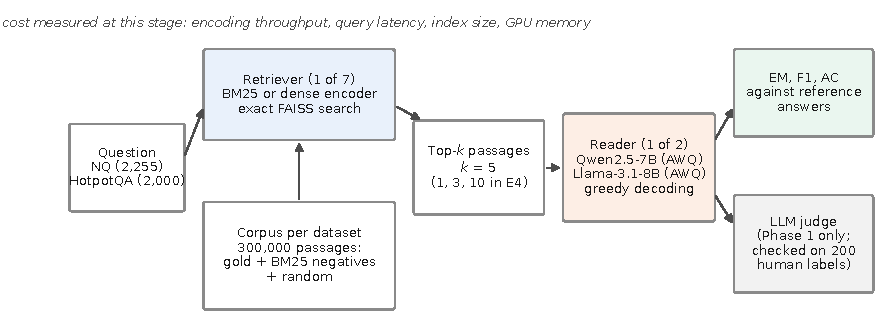
\includegraphics[width=\linewidth]{figs/fig7_system.pdf}
\caption{System under test. Within a reader--dataset cell only the retriever changes. Cost is measured at the retrieval stage. The LLM judge was used only in Phase~1 and was later excluded (Section~\ref{sec:res-judge}).}
\label{fig:system}
\end{figure}

\subsection{Transfer ratio}\label{sec:ratio}
Let $Q$ be a fixed set of generation queries. For retriever $R$ and query $q$, let $h_R(q)\in\{0,1\}$ indicate that at least one gold passage of $q$ is among the top five passages, and let $e_R(q)\in\{0,1\}$ be the exact match of the reader's answer given those five passages. Write $\bar h_R$ and $\bar e_R$ for the means over $Q$. With MiniLM-L6 as the baseline $R_1$, the transfer ratio is
\begin{equation}
T(R) = \frac{\bar e_R - \bar e_{R_1}}{\bar h_R - \bar h_{R_1}}.
\label{eq:ratio}
\end{equation}
Both differences are paired: they use the same queries, the same reader, the same prompt and the same decoding. $T(R)$ is a ratio of mean differences. It is not the probability that one extra hit produces one extra correct answer, because the queries that gain a hit need not be the queries that gain an answer. We report $T(R)$ only if $|\bar h_R-\bar h_{R_1}|$ exceeds 2 percentage points and the Hit@5 difference is significant after Holm correction; otherwise the ratio is marked as not estimable. This rule was fixed in the Phase~1 design to avoid ratios with near-zero denominators. $T(R)$ depends on the choice of $R_1$. As a post hoc sensitivity analysis we therefore repeat every ratio with BM25 as the baseline, under the same rule.

\paragraph{Decomposition}
Let $a_R=P(e_R=1\mid h_R=1)$ and $b_R=P(e_R=1\mid h_R=0)$ be the EM rates among hits and misses. Then $\bar e_R=\bar h_R a_R+(1-\bar h_R)b_R$, and Eq.~\ref{eq:ratio} splits exactly into
\begin{equation}
T(R) = \underbrace{(a_{R_1}-b_{R_1})}_{\text{baseline hit--miss gap}} + \underbrace{\frac{\bar h_R\,(a_R-a_{R_1}) + (1-\bar h_R)\,(b_R-b_{R_1})}{\bar h_R-\bar h_{R_1}}}_{\text{change in conditional EM}}.
\label{eq:decomp}
\end{equation}
If a better encoder only turned misses into hits and left $a$ and $b$ unchanged, $T(R)$ would equal the baseline gap. The second term measures how far the encoder also changes the usefulness of its hits and misses. We report the share of the EM gain that the second term carries, $[\bar h_R(a_R-a_{R_1})+(1-\bar h_R)(b_R-b_{R_1})]/(\bar e_R-\bar e_{R_1})$, with a bootstrap interval over the same resamples as $T(R)$. The split is not unique. Eq.~\ref{eq:decomp} weights the change in hit rate by the baseline's conditional rates; a symmetric form averages the two orderings of $R_1$ and $R$, and we report it alongside. Either form is an accounting identity, not a causal attribution: the queries that count as hits differ between encoders, so a change in $a$ can reflect which questions are hits as well as how useful a hit is. This decomposition was not part of the registered analysis; we report it as a post hoc description.

\subsection{Data}\label{sec:data}
\paragraph{Natural Questions}
We used the BEIR version of Natural Questions \citep{kwiatkowski2019nq,thakur2021beir}: \ev{N.nq.judged} judged test queries and a corpus of 2,681,468 Wikipedia passages. BEIR does not ship short answers, so we joined its queries to NQ-open \citep{lee2019orqa} by normalised question text. The join matched \ev{N.nq.joined} queries; \ev{N.nq.unmatched} had no match and none had more than one. All \ev{N.nq.joined} joined queries form the NQ generation set. Table~\ref{tab:data} in the appendix summarises both datasets and sub-corpora.

\paragraph{HotpotQA}
We used the BEIR version of HotpotQA \citep{yang2018hotpotqa,thakur2021beir}: \ev{N.hp.judged} judged test queries, two gold passages per query, and a corpus of 5,233,329 passages. Answers come from the fullwiki validation release, joined by question id; all queries matched. The generation set is the leading \ev{N.hp.gen} queries of a seeded order (\ev{N.qhp.bridge} bridge and \ev{N.qhp.comparison} comparison questions).

\paragraph{Sub-corpus}
Encoding millions of passages with six encoders exceeds a free GPU budget, so each dataset uses a 300,000-passage sub-corpus. It contains the gold passages of all judged queries, the top-$d$ BM25 passages of every judged query ($d$ = 42 for NQ and 19 for HotpotQA, set by a pre-registered formula), and a seeded random fill. All retrievers search the same sub-corpus. The NQ sub-corpus has \ev{N.sc.nq.gold} gold, \ev{N.sc.nq.bm25} BM25 and \ev{N.sc.nq.rand} random passages; the HotpotQA sub-corpus has \ev{N.sc.hp.gold}, \ev{N.sc.hp.bm25} and \ev{N.sc.hp.rand}. Because every gold passage is present, absolute retrieval scores are higher than on the full corpus. The construction also treats the retrievers unequally: it keeps BM25's own strongest competitors for every judged query, but not those of the dense encoders, so it favours the dense encoders relative to BM25. The gold labels of the evaluation queries are used only to insert their gold passages; no model is trained on them. Section~\ref{sec:res-cost} checks whether the ordering of retrievers changes.

\subsection{Retrievers}\label{sec:retrievers}
BM25 used the bm25s library \citep{lu2024bm25s} with the Lucene variant, $k_1=1.2$, $b=0.75$, lower-casing and no stemming or stop-word removal \citep{robertson2009bm25}. The six dense encoders were all-MiniLM-L6-v2 \citep{reimers2019sbert,wang2020minilm}, bge-small, bge-base and bge-large v1.5 \citep{xiao2024cpack}, e5-base-v2 \citep{wang2022e5} and Qwen3-Embedding-0.6B \citep{zhang2025qwen3emb}. Each model ran at a pinned revision in half precision with a maximum of 256 tokens and its documented query and passage prefixes. Dense search used exact inner-product search in FAISS \citep{johnson2021faiss}. Table~\ref{tab:models} in the appendix lists the models, revisions and prefixes.

\subsection{Readers and prompts}\label{sec:readers}
The readers were Qwen2.5-7B-Instruct \citep{qwen2025qwen25} and Llama-3.1-8B-Instruct \citep{grattafiori2024llama3}, both in 4-bit AWQ form \citep{lin2024awq}, served with vLLM \citep{kwon2023vllm} on one T4 each. Decoding was greedy with at most 32 new tokens and a stop at a newline. The main prompt (A1) gives the top $k=5$ passages in rank order, each as ``[i] title / text'', and asks for a short answer (Appendix~\ref{app:prompts}). Two reference conditions bound each cell: closed book (no passages) and gold passages only.

\subsection{Metrics}\label{sec:metrics}
Hit@5 is 1 if at least one gold passage is in the top five. For HotpotQA we also report Both@5, which requires both gold passages. nDCG@10 uses binary gains. EM is 1 if the normalised answer equals a normalised reference answer. Normalisation follows SQuAD (lower case, no punctuation or articles, single spaces) and also removes typographic quotes, en and em dashes and the ellipsis; a plain SQuAD normaliser would change the score of \ev{IC.plain} of \ev{IC.n} answers (\ev{IC.plainpct}). Token F1 and answer containment (AC; a normalised reference occurs in the normalised output) are secondary metrics, because lexical EM undercounts correct answers from language models \citep{kamalloo2023}.

\subsection{Statistical analysis}\label{sec:stats}
All comparisons are paired by query. Binary outcomes use the exact McNemar test \citep{mcnemar1947}. Within each reader--dataset cell, the 21 pairwise retriever comparisons of a metric form one family with Holm correction \citep{holm1979}. Intervals are 95\% percentile bootstrap intervals over queries \citep{efron1993bootstrap} with 10,000 resamples and seed 0; for $T(R)$ the numerator and denominator are resampled together. A secondary model pools the four cells: a logistic generalised estimating equation \citep{liang1986gee} for EM with retriever, dataset and reader as factors, an exchangeable working correlation within query, and empirical (sandwich) standard errors. The cluster is the query, which carries all retrievers and both readers of its dataset. This registered model assumes one retriever effect for both datasets. Post hoc, we test that assumption with a Wald test of retriever $\times$ dataset interaction terms (and of retriever $\times$ reader terms) and report dataset-specific odds ratios from the interaction model. Agreement between the LLM judge and human labels uses Cohen's $\kappa$ \citep{cohen1960kappa,landis1977}. A non-significant test is reported as ``no difference detected'', not as equivalence.

\subsection{Pre-registered predictions}\label{sec:prereg}
Phase~1 (Qwen reader, NQ) was designed and committed before any data were generated. Before Phase~2 we registered six predictions (Table~\ref{tab:predictions}):
\begin{description}
\item[P1] In each new cell, every reportable $T(R)$ of a dense encoder has an upper 95\% bound below 1.
\item[P2] In each new cell, bge-large and Qwen3-Embedding-0.6B show no Holm-significant EM gain over e5-base-v2.
\item[P3] The nDCG@10 ordering of BM25, MiniLM-L6, bge-small and e5-base-v2 on the sub-corpus holds on the full corpus.
\item[P4] For every retriever, EM at $k=1$ is lower than at $k=5$.
\item[P5] Gold plus four hard negatives gives lower EM than gold plus four random passages.
\item[P6] The position of the gold passage (1, 3 or 5) changes EM.
\end{description}
Fig.~\ref{fig:phases} shows the sessions of both phases. The Qwen--NQ cell and the $k$ ablation for BM25, MiniLM-L6 and bge-large existed before registration. Their P1, P2 and P4 verdicts are therefore not confirmatory, and Table~\ref{tab:predictions} marks them. All other analyses are descriptive or secondary. Appendix~\ref{app:prereg} lists the design documents and their dates.

\begin{figure}[t]
\centering
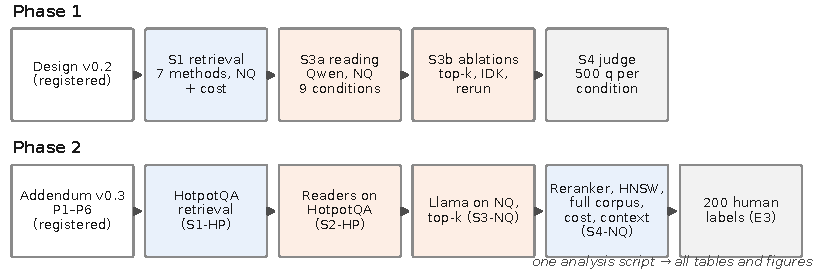
\includegraphics[width=\linewidth]{figs/fig8_phases.pdf}
\caption{Study phases and Kaggle sessions. Each phase started with a dated design document; Phase~2 added the second dataset, the second reader and the additional experiments.}
\label{fig:phases}
\end{figure}

\subsection{Additional experiments}\label{sec:extra}
\paragraph{Top-$k$ (E4)} The Qwen reader answered all NQ queries with $k\in\{1,3,5,10\}$ for all seven retrievers.
\paragraph{Context composition (E12)} On the leading 500 NQ generation queries of the seeded order, the Qwen reader always saw five passages: gold at position 1 plus four hard negatives (M1); gold at position 3 or 5 among the same negatives (M3, M5); gold at position 1 plus four random passages (MR); and the gold passage alone (MG). Hard negatives are the top-ranked BM25 passages that are not labelled gold.
\paragraph{Reranking (E5)} A cross-encoder, bge-reranker-base, reranked the top 50 passages of BM25 and of e5-base-v2 \citep{nogueira2019passage,xiao2024cpack}; the Qwen reader then answered NQ from the reranked top five.
\paragraph{Approximate search (E6)} HNSW indexes \citep{malkov2020hnsw} ($M=32$, efConstruction 200, efSearch 64 and 128) replaced exact search for MiniLM-L6, bge-small and e5-base-v2 on the NQ sub-corpus.
\paragraph{Full corpus (E9)} BM25, MiniLM-L6, bge-small and e5-base-v2 retrieved from the full NQ corpus for all judged queries.
\paragraph{Cost (E7)} For each encoder we measured passage-encoding throughput on 20,000 passages (batch 128, after warm-up, with GPU synchronisation) and batch-1 query-encoding latency on 500 queries, five times in one session.
\paragraph{Judge validation (E3)} In Phase~1, an LLM judge (Mistral-7B-Instruct-v0.3; \citealp{jiang2023mistral}) labelled whether each answer was supported by its passages, for 500 NQ queries per retriever. The author labelled a stratified sample of 200 items without seeing the judge's verdicts. The registered rule was: use the judge if $\kappa\ge0.4$, use it only with a sensitivity analysis if $0.2\le\kappa<0.4$, and exclude it if $\kappa<0.2$.

\section{Experimental setup}\label{sec:setup}

\paragraph{Hardware and software}
All runs used free Kaggle notebook sessions with two NVIDIA Tesla T4 GPUs (15 GB each), four virtual CPUs and 31.3 GiB of memory. Each process used one GPU; two processes could run in parallel. The code of every session was embedded in its notebook and checked against a fixed version-control tree hash before it ran. Every session recorded its Python version, package versions and model revisions. The readers ran with the same stack in every session (PyTorch 2.13.0 with CUDA 13.0, vLLM 0.30.0, Transformers 5.17.0). Between Phases~1 and~2 the Kaggle image changed from Python 3.12.13 to 3.13.15, and NumPy from 2.0.2 to 2.1.3; Phase~3 used the same image and package versions as Phase~2. The two sessions that encoded the NQ and HotpotQA sub-corpora used older images (PyTorch 2.10.0 and 2.11.0 with CUDA 12.8, Transformers 5.0.0); Table~\ref{tab:env} lists the software of every session as its environment log recorded it.

\paragraph{Determinism across phases}
Some comparisons cross Phases~1 and~2: the Qwen--NQ cell against the new cells in the pooled model, $k=5$ against the new $k$ values, the reranker runs against the Phase~1 runs, and the Phase~3 runs of the Qwen reader against its Phase~1 sub-corpus runs. To check that the software change does not alter the reader, we compared Phases~1 and~2 on inputs that were identical by construction: the gold-only context of Phase~1 and the gold-only condition of the context experiment. Of \ev{CS.n} identical prompts, \ev{CS.same} produced identical outputs; the one difference was a shorter answer to the same question. A rerun of 100 prompts within one session gave \ev{CS.within} identical outputs.

\paragraph{Seeds and repetitions}
The query order (seed 20260926), bootstrap (seed 0), decoding (greedy, seed 0) and the random passages of the context experiment were fixed. Retrieval and greedy decoding are deterministic within a session, so we ran each answer condition once. The cost measurements were repeated five times.

\paragraph{Analysis and verification}
One analysis script reads only the committed raw outputs and writes all statistics, tables and figures. The author reran it on a second computer and obtained identical output. A separate script, written without the project code and using only the Python standard library, re-scored all \ev{IC.n} answers from the raw reader outputs, recomputed every Hit@5 and EM mean, every transfer ratio point estimate, all 84 pairwise EM tests with their Holm adjustment, and Cohen's $\kappa$. It found no disagreement. Bootstrap intervals, F1, answer containment and the pooled model were not re-implemented independently. Phase~3 has its own analysis script, which also reads only committed outputs. It checks that the passages each reader saw equal the top five of the stored ranked lists, and that the sub-corpus intervals it recomputes equal the committed ones. Re-encoding the full corpus gave Hit@5 and nDCG@10 values \ev{V6.e9.repro} to those of the earlier full-corpus check (E9) for all four retrievers. A second script, again written without the project code, re-scored all \ev{V6.n.gen} Phase~3 answers from the raw reader outputs and recomputed the means, ratios with their intervals, McNemar tests, query-level contributions and the answer-string shares of MiniLM-L6 and e5-base-v2; it found no disagreement.

\subsection{Deviations and failed runs}\label{sec:deviations}
We list every departure from the registered design.
\begin{enumerate}
\item \textbf{NQ join gate.} The original design required a join rate of at least 0.70 between BEIR-NQ and NQ-open; the observed rate was \ev{N.nq.joinrate}. Before any outcome was observed, we replaced the gate with a minimum of 1,000 joined queries, because the two resources are independently filtered subsets of Natural Questions. Retrieval results on all \ev{N.nq.judged} judged queries are reported where they matter (Table~\ref{tab:fullcorpus}).
\item \textbf{Software image.} The initial Phase~2 session stopped at the environment check because the Kaggle image had moved to Python 3.13, for which the pinned NumPy had no wheel. We unpinned NumPy and recorded all version differences; no data were produced by the stopped run.
\item \textbf{Failed reader start.} The initial HotpotQA reader session stopped before generating anything because the image's torchaudio build did not match the CUDA version of PyTorch. Later sessions reinstalled the matching build and checked the stack before any other step.
\item \textbf{Reduced scope of E6.} Approximate search was planned for all six encoders. To stay within the GPU quota it ran for MiniLM-L6, bge-small and e5-base-v2, using the sub-corpus rows of the full-corpus embeddings.
\item \textbf{E7 scope.} The repeated cost measurement covered encoding throughput and query-encoding latency; search latency was measured separately in E6 and is not repeated.
\item \textbf{Phase~1 deviations.} We dropped the planned RAGAS cross-check, because its local deployment needed infrastructure that was untested on our hardware. We did not run the planned Matryoshka dimension ablation for Qwen3-Embedding-0.6B, so dimension and model are confounded in our cost comparison. The design planned two annotators for the judge validation; one took part. One gold-passage output reached the token limit, so the judge scored 499 instead of 500 gold items. The initial Phase~1 reading session stopped before generating because a notebook cell ran before the restore step; it was rerun with unchanged code. We estimated the Phase~1 CPU benchmark at one hour; it took eight hours and 24 minutes. This used free quota but changed no data.
\item \textbf{Failure log.} The design promised one machine-readable failure log. Failures were recorded instead in two dated design addenda and in the session logs.
\item \textbf{Phase~3 human audit.} The Phase~3 design adds a blinded audit of 100 seeded e5-base-v2 retrieval misses by the author. Its labels were not complete when this version was written, so it is not reported. The Phase~3 session itself ran as registered, with no failed run.
\end{enumerate}
No run was repeated to obtain a different result, and no result was discarded.

\section{Results}\label{sec:results}

\subsection{Retrieval}\label{sec:res-retrieval}
Table~\ref{tab:retrieval} gives retrieval quality on the generation queries, and Table~\ref{tab:ci} gives the intervals. On NQ, the dense encoders differed widely. MiniLM-L6 reached \ev{HIT.nq.R1} and e5-base-v2 \ev{HIT.nq.R5}; bge-large (\ev{HIT.nq.R4}) came second. Qwen3-Embedding-0.6B (\ev{HIT.nq.R6}) placed between bge-small and bge-base. BM25 reached \ev{HIT.nq.R0}. On HotpotQA, Hit@5 nearly saturated: all dense encoders except MiniLM-L6 scored between \ev{HIT.hp.R6} and \ev{HIT.hp.R4}, against \ev{HIT.hp.R1} for MiniLM-L6 and \ev{HIT.hp.R0} for BM25. The stricter Both@5 separated them more clearly: bge-large found both supporting passages for \ev{BOTH.hp.R4} of the questions, e5-base-v2 for \ev{BOTH.hp.R5}, Qwen3-Embedding-0.6B for \ev{BOTH.hp.R6} and MiniLM-L6 for \ev{BOTH.hp.R1}. Table~\ref{tab:retrieval} also gives Hit@1, Hit@10, nDCG@10 and MRR@10, and Fig.~\ref{fig:retrieval} shows the main metrics with their intervals. On NQ, nDCG@10 ordered the retrievers as Hit@5 did, from \ev{RET.nq.ndcg10.R0} for BM25 and \ev{RET.nq.ndcg10.R1} for MiniLM-L6 to \ev{RET.nq.ndcg10.R5} for e5-base-v2. On HotpotQA, nDCG@10 ranged from \ev{RET.hp.ndcg10.R1} (MiniLM-L6) to \ev{RET.hp.ndcg10.R4} (bge-large).

\begin{figure}[t]
\centering
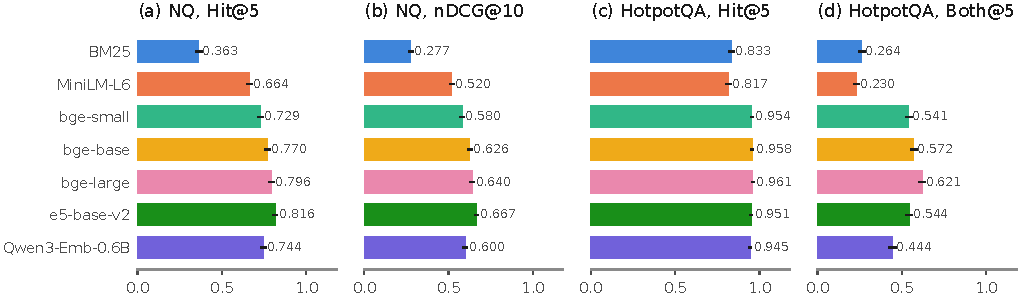
\includegraphics[width=\linewidth]{figs/fig9_retrieval.pdf}
\caption{Retrieval quality on the generation queries with 95\% bootstrap intervals: NQ Hit@5 and nDCG@10 (2,255 queries), HotpotQA Hit@5 and Both@5 (2,000 queries).}
\label{fig:retrieval}
\end{figure}

\begin{table*}[t]
\centering
\footnotesize
\setlength{\tabcolsep}{3.5pt}
\caption{Retrieval quality on the generation queries of each dataset (300,000-passage sub-corpora, exact search).}
\label{tab:retrieval}
\begin{tabular}{lcccccccccc}
\toprule
 & \multicolumn{5}{c}{NQ (2,255 queries)} & \multicolumn{5}{c}{HotpotQA (2,000 queries)} \\ \cmidrule(lr){2-6}\cmidrule(lr){7-11}
Retriever & Hit@1 & Hit@5 & Hit@10 & nDCG@10 & MRR@10 & Hit@1 & Hit@5 & Both@5 & nDCG@10 & MRR@10 \\
\midrule
BM25 & 0.150 & 0.363 & 0.472 & 0.277 & 0.243 & 0.666 & 0.833 & 0.264 & 0.578 & 0.740 \\
MiniLM-L6 & 0.316 & 0.664 & 0.792 & 0.520 & 0.462 & 0.623 & 0.817 & 0.230 & 0.549 & 0.708 \\
bge-small & 0.375 & 0.729 & 0.843 & 0.580 & 0.526 & 0.812 & 0.954 & 0.541 & 0.756 & 0.874 \\
bge-base & 0.421 & 0.770 & 0.882 & 0.626 & 0.570 & 0.836 & 0.958 & 0.572 & 0.777 & 0.888 \\
bge-large & 0.430 & 0.796 & 0.888 & 0.640 & 0.584 & 0.846 & 0.961 & 0.621 & 0.797 & 0.897 \\
e5-base-v2 & 0.458 & 0.816 & 0.906 & 0.667 & 0.612 & 0.799 & 0.951 & 0.544 & 0.751 & 0.864 \\
Qwen3-Emb-0.6B & 0.400 & 0.744 & 0.843 & 0.600 & 0.547 & 0.810 & 0.945 & 0.444 & 0.717 & 0.868 \\
\bottomrule
\end{tabular}
\par\smallskip\parbox{\linewidth}{\footnotesize NQ intervals for Hit@5 and nDCG@10 are in Table~\ref{tab:ci} and Fig.~\ref{fig:retrieval}. Both@5: both gold passages in the top five.}
\end{table*}


\subsection{Answer gains and transfer ratios (RQ1)}\label{sec:res-transfer}
Table~\ref{tab:main} gives EM for every cell with its two reference conditions, and Fig.~\ref{fig:hitem} plots EM against Hit@5. Retrieval closed only part of the gap between the closed-book and gold-passage conditions. With Qwen on NQ, closed-book EM was \ev{EM.qnq.CB}, gold passages gave \ev{EM.qnq.GOLD}, and the best retriever, e5-base-v2, gave \ev{EM.qnq.R5}. With Llama on NQ the best retriever was bge-base (\ev{EM.lnq.R3}) against a gold-passage reference of \ev{EM.lnq.GOLD}. On HotpotQA, bge-large gave the highest EM for both readers (\ev{EM.qhp.R4} and \ev{EM.lhp.R4}), against gold-passage references of \ev{EM.qhp.GOLD} and \ev{EM.lhp.GOLD}.

\begin{figure}[t]
\centering
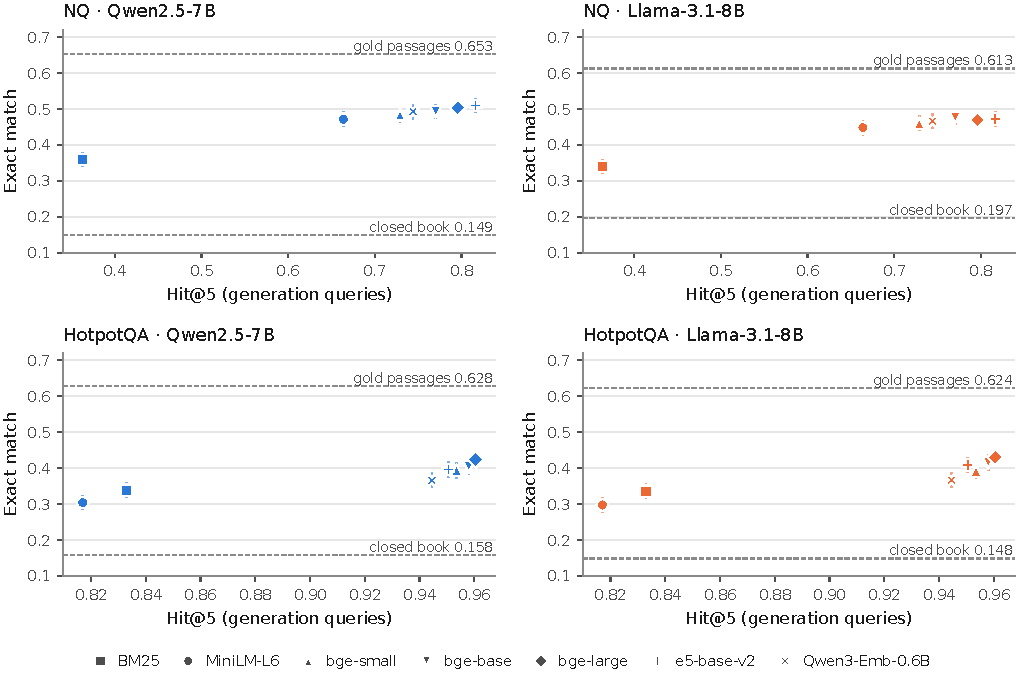
\includegraphics[width=\linewidth]{figs/fig2_hit_vs_em.pdf}
\caption{Exact match against Hit@5 for each retriever in the four reader--dataset cells. Vertical bars are 95\% bootstrap intervals for EM. Dashed lines mark the closed-book and gold-passage reference conditions. Note the different Hit@5 ranges of the two datasets.}
\label{fig:hitem}
\end{figure}

Table~\ref{tab:transfer} and Fig.~\ref{fig:transfer} give the transfer ratios. On NQ, the five dense encoders had ratios between \ev{T.lnq.R4} (bge-large and e5-base-v2 with Llama) and \ev{T.lnq.R3} (bge-base with Llama). With Qwen, e5-base-v2 gained \ev{DH.qnq.R5} in Hit@5 over MiniLM-L6 but only \ev{DE.qnq.R5} in EM, a ratio of \ev{T.qnq.R5} \ev{T.qnq.R5.ci}. The intervals for bge-small included zero in both NQ cells (Qwen \ev{T.qnq.R2.ci}, Llama \ev{T.lnq.R2.ci}), so its NQ ratio is uncertain in sign. The largest NQ upper bound was \ev{V5.nq.ubmax} (Qwen3-Embedding-0.6B with Qwen). BM25 retrieved worse than MiniLM-L6 on NQ, so its ratio (\ev{T.qnq.R0} with Qwen) relates an EM loss to a Hit@5 loss.

With Hit@5 as the denominator, the HotpotQA ratios were larger for every encoder and reader, from \ev{T.qhp.R6} (Qwen3-Embedding-0.6B with Qwen) to \ev{T.lhp.R4} (bge-large with Llama). With Qwen, every upper bound stayed below 1, the largest being \ev{T.qhp.R4.hi3} for bge-large. With Llama, the bounds were \ev{T.lhp.R3.hi3} for bge-base, \ev{T.lhp.R5.hi3} for e5-base-v2 and \ev{T.lhp.R4.hi3} for bge-large, so the P1 criterion (every upper bound below 1) was met in the two new NQ and Qwen--HotpotQA cells and not met in the Llama--HotpotQA cell (Table~\ref{tab:predictions}). The BM25 ratio was not estimable on HotpotQA, because BM25 and MiniLM-L6 differed by only \ev{DH.qhp.R0} in Hit@5.

\begin{figure}[t]
\centering
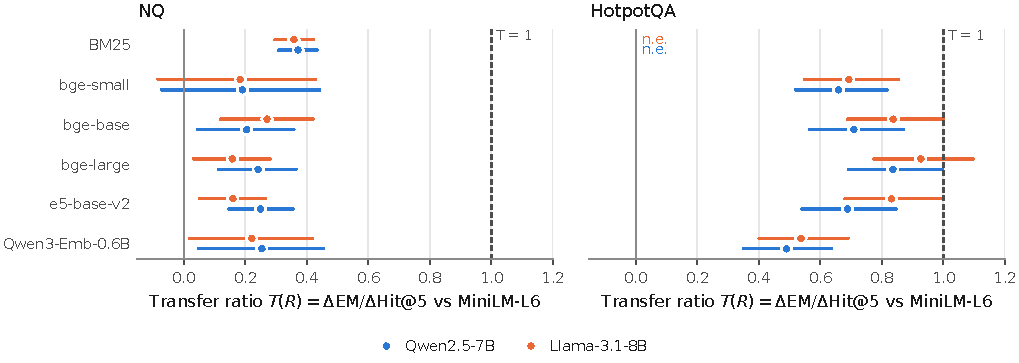
\includegraphics[width=\linewidth]{figs/fig1_transfer_ratios.pdf}
\caption{Transfer ratio $T(R)=\Delta\mathrm{EM}/\Delta\mathrm{Hit@5}$ against MiniLM-L6 with 95\% bootstrap intervals. The dashed line marks $T=1$, a reference point. n.e.: not estimable under the reporting rule.}
\label{fig:transfer}
\end{figure}

\begin{table*}[t]
\centering
\small
\caption{Retrieval (Hit@5) and answer quality (exact match) for each reader and dataset. Hit@5 is computed on the generation queries; 95\% bootstrap intervals are in Table~\ref{tab:ci}.}
\label{tab:main}
\begin{tabular}{lrrrrrrrr}
\toprule
 & \multicolumn{4}{c}{NQ (2,255 queries)} & \multicolumn{4}{c}{HotpotQA (2,000 queries)} \\ \cmidrule(lr){2-5}\cmidrule(lr){6-9} & \multicolumn{2}{c}{Qwen} & \multicolumn{2}{c}{Llama} & \multicolumn{2}{c}{Qwen} & \multicolumn{2}{c}{Llama} \\ \cmidrule(lr){2-3}\cmidrule(lr){4-5}\cmidrule(lr){6-7}\cmidrule(lr){8-9}
Retriever & Hit@5 & EM & Hit@5 & EM & Hit@5 & EM & Hit@5 & EM \\
\midrule
BM25 & 0.363 & 0.360 & 0.363 & 0.340 & 0.833 & 0.339 & 0.833 & 0.336 \\
MiniLM-L6 & 0.664 & 0.471 & 0.664 & 0.448 & 0.817 & 0.304 & 0.817 & 0.297 \\
bge-small & 0.729 & 0.484 & 0.729 & 0.460 & 0.954 & 0.394 & 0.954 & 0.392 \\
bge-base & 0.770 & 0.493 & 0.770 & 0.477 & 0.958 & 0.404 & 0.958 & 0.415 \\
bge-large & 0.796 & 0.503 & 0.796 & 0.469 & 0.961 & 0.424 & 0.961 & 0.430 \\
e5-base-v2 & 0.816 & 0.510 & 0.816 & 0.472 & 0.951 & 0.396 & 0.951 & 0.408 \\
Qwen3-Emb-0.6B & 0.744 & 0.492 & 0.744 & 0.466 & 0.945 & 0.366 & 0.945 & 0.366 \\
Closed book & -- & 0.149 & -- & 0.197 & -- & 0.158 & -- & 0.148 \\
Gold passages & -- & 0.653 & -- & 0.613 & -- & 0.628 & -- & 0.624 \\
\bottomrule
\end{tabular}
\end{table*}

\begin{table*}[t]
\centering
\small
\caption{Transfer ratio $T(R)=\Delta\mathrm{EM}/\Delta\mathrm{Hit@5}$ relative to MiniLM-L6, with 95\% bootstrap intervals.}
\label{tab:transfer}
\begin{tabular}{lcccc}
\toprule
Retriever & NQ Qwen & NQ Llama & HotpotQA Qwen & HotpotQA Llama \\
\midrule
BM25 & 0.37 [0.31, 0.43] & 0.36 [0.30, 0.42] & n.e. & n.e. \\
bge-small & 0.19 [$-$0.07, 0.44] & 0.18 [$-$0.08, 0.43] & 0.66 [0.52, 0.82] & 0.69 [0.55, 0.85] \\
bge-base & 0.20 [0.04, 0.36] & 0.27 [0.12, 0.42] & 0.71 [0.57, 0.87] & 0.84 [0.69, 1.00] \\
bge-large & 0.24 [0.11, 0.36] & 0.16 [0.03, 0.28] & 0.84 [0.69, 1.00] & 0.93 [0.78, 1.10] \\
e5-base-v2 & 0.25 [0.15, 0.36] & 0.16 [0.05, 0.26] & 0.69 [0.54, 0.85] & 0.83 [0.68, 1.00] \\
Qwen3-Emb-0.6B & 0.25 [0.05, 0.45] & 0.22 [0.02, 0.42] & 0.49 [0.35, 0.64] & 0.54 [0.40, 0.69] \\
\bottomrule
\end{tabular}
\par\smallskip\parbox{\linewidth}{\footnotesize n.e.: not estimable under the pre-registered rule ($|\Delta\mathrm{Hit@5}|\le 2$ points or not significant after Holm). BM25 on NQ retrieves worse than MiniLM-L6, so its ratio describes a loss.}
\end{table*}


\subsection{How stable are the ratios?}\label{sec:res-sens}
Table~\ref{tab:sensitivity} repeats the dense-encoder ratios under other answer metrics, another baseline, another retrieval metric and other numbers of passages. Only the top row is the registered analysis.

On NQ, one pattern held in every row read at $k\geq 3$: each ratio and each upper bound stayed well below 1. With token F1 the NQ ratios were \ev{V5.f1.nq}, with answer containment \ev{V5.ac.nq}, and against BM25 instead of MiniLM-L6 \ev{V4.b0.nq.min}--\ev{V4.b0.nq.max}; the largest upper bound over these rows was \ev{V5.nq.allub}. The size of the ratio was not stable, however. It fell with the number of passages read: \ev{V5.k1.range} at $k=1$, \ev{V5.k3.range} at $k=3$ and \ev{V5.k10.range} at $k=10$ (Qwen; exploratory, Hit@$k$ matched to $k$). At $k=1$ the largest upper bound was \ev{V5.k1.ubmax}.

On HotpotQA, the size of the ratio depended mainly on the retrieval metric. With Both@5 instead of Hit@5 as the denominator, the dense-encoder ratios were \ev{V4.both.hp.min}--\ev{V4.both.hp.max} for both readers, close to the NQ ratios against BM25, and Qwen3-Embedding-0.6B no longer stood apart. Against BM25 with Hit@5, the HotpotQA ratios were \ev{V4.b0.hp.min}--\ev{V4.b0.hp.max}; they exceeded the NQ ratios in \ev{V4.b0.hpgt} of 10 encoder--reader pairs, the exceptions being Qwen3-Embedding-0.6B (\ev{V4.b0.qwen_hp.R6} and \ev{V4.b0.llama_hp.R6} against \ev{V4.b0.qwen_nq.R6} and \ev{V4.b0.llama_nq.R6}). Under F1, the Llama ratio of bge-large was \ev{TF.lhp.R4} \ev{TF.lhp.R4.ci}, so full transfer cannot be ruled out for that encoder when it is measured with Hit@5.

The stable finding is therefore that, with three to ten passages read ($k$ = 3, 5 and 10), a Hit@5 gain over a small encoder bought a much smaller EM gain on NQ. The exact ratio depends on the baseline, the answer metric and $k$, and the larger HotpotQA ratios depend on scoring retrieval by any rather than all supporting passages.

\begin{table*}[t]
\centering
\small
\caption{Sensitivity of the dense-encoder transfer ratios (range over five encoders and both readers unless stated). All rows except the top one are secondary or post hoc.}
\label{tab:sensitivity}
\begin{tabular}{lcccc}
\toprule
Answer metric, retrieval metric, baseline & NQ ratios & NQ max. upper & HotpotQA ratios & HotpotQA max. upper \\
\midrule
EM (primary), Hit@5, MiniLM-L6 & 0.16--0.27 & 0.45 & 0.49--0.93 & 1.10 \\
token F1, Hit@5, MiniLM-L6 & 0.23--0.33 & 0.49 & 0.52--1.10 & 1.28 \\
answer containment, Hit@5, MiniLM-L6 & 0.27--0.39 & 0.60 & 0.49--1.01 & 1.18 \\
EM, Hit@5, BM25 & 0.29--0.35 & 0.40 & 0.25--0.75 & 0.92 \\
EM, Both@5, MiniLM-L6 & -- & -- & 0.29--0.35 & 0.41 \\
EM, Hit@$k$ at $k=1$, MiniLM-L6 (Qwen) & 0.41--0.83 & 1.22 & -- & -- \\
EM, Hit@$k$ at $k=3$, MiniLM-L6 (Qwen) & 0.32--0.37 & 0.59 & -- & -- \\
EM, Hit@$k$ at $k=10$, MiniLM-L6 (Qwen) & 0.05--0.19 & 0.42 & -- & -- \\
\bottomrule
\end{tabular}
\par\smallskip\parbox{\linewidth}{\footnotesize Max. upper: largest upper 95\% bootstrap bound in the row. The $k$ rows match Hit@$k$ to the $k$ passages read (Qwen reader, NQ only; exploratory, without the reporting rule).}
\end{table*}


\subsection{Do the NQ ratios hold on the full corpus?}\label{sec:res-full}
All results so far use the 300,000-passage sub-corpus, which favours the dense encoders relative to BM25. In Phase~3 both readers answered the NQ generation queries from retrieval on the full corpus of \ev{V6.enc.rows} passages (Table~\ref{tab:fullreader} and Fig.~\ref{fig:fulltransfer}). On the full corpus the dense encoders lost \ev{V6.dHit.dense.abs} in Hit@5 and \ev{V6.dEM.dense.abs} in EM (all Holm-adjusted $p\le$ \ev{V6.dEM.dense.pmax}). BM25 kept its Hit@5, and its EM changed by no detectable amount (\ev{V6.dEM.R0}; $p\ge$ \ev{V6.dEM.R0.pmin}).

The transfer ratios hardly moved. With e5-base-v2, $T$ was \ev{V6.T3.q.R5} \ev{V6.T.q.R5.ci} with Qwen, inside its sub-corpus interval \ev{V6.P8.q.sub}, and \ev{V6.T3.l.R5} \ev{V6.T.l.R5.ci} with Llama, inside \ev{V6.P8.l.sub}. The paired differences from the sub-corpus ratios were \ev{V6.dT.q} \ev{V6.dT.q.ci} and \ev{V6.dT.l} \ev{V6.dT.l.ci}. The bge-small ratios were \ev{V6.T.q.R2} \ev{V6.T.q.R2.ci} and \ev{V6.T.l.R2} \ev{V6.T.l.R2.ci}; as on the sub-corpus, their intervals included zero. Every dense upper bound stayed below 1 (largest \ev{V6.T.ubmax}), so P7 and P8 were met for both readers. Against BM25, the ratios of bge-small and e5-base-v2 were \ev{V6.b0.full} on the full corpus and \ev{V6.b0.sub} on the sub-corpus.

The query-level accounting also kept its shape. Queries that moved from miss to hit contributed \ev{V6.tr.misshit.contrib} to the EM gain, those that hit under both retrievers \ev{V6.tr.hithit.contrib} (interval below zero in \ev{V6.tr.hithit.neg} of 4 encoder--reader pairs) and those that lost their hit \ev{V6.tr.hitmiss.contrib}. In a comparison that was not pre-specified, the full corpus cost the three dense encoders \ev{V6.lossratio} EM points per Hit@5 point lost, about the size of the transfer ratios themselves. At most \ev{V6.unparsed.max} of the full-corpus outputs could not be parsed.

\begin{figure}[t]
\centering
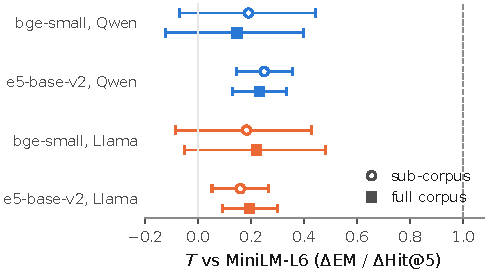
\includegraphics[width=0.75\linewidth]{figs/fig13_fullcorpus_T.pdf}
\caption{NQ transfer ratios against MiniLM-L6 on the sub-corpus (open circles) and on the full corpus (filled squares), with 95\% bootstrap intervals; 2,255 queries, $k=5$. The dashed line marks $T=1$.}
\label{fig:fulltransfer}
\end{figure}

\begin{table*}[t]
\centering
\footnotesize
\caption{NQ readers on the 300,000-passage sub-corpus and on the full 2,681,468-passage corpus (Phase 3), 2,255 generation queries, $k=5$. Intervals are 95\% bootstrap intervals.}
\label{tab:fullreader}
\begin{tabular}{lccccccll}
\toprule
& \multicolumn{2}{c}{Hit@5} & \multicolumn{2}{c}{EM} & & & \multicolumn{2}{c}{$T$ vs MiniLM-L6 [95\% CI]} \\ \cmidrule(lr){2-3}\cmidrule(lr){4-5}\cmidrule(lr){8-9} Retriever & sub & full & sub & full & $\Delta$EM full$-$sub & $p_\text{Holm}$ & sub & full \\
\midrule
\multicolumn{9}{l}{\textit{Qwen2.5-7B}} \\
BM25 & 0.363 & 0.364 & 0.360 & 0.358 & \ensuremath{-}0.001 & 0.798 & 0.37 [0.31, 0.43] & 0.44 [0.35, 0.53] \\
MiniLM-L6 & 0.664 & 0.564 & 0.471 & 0.446 & \ensuremath{-}0.025 & $<$0.001 & -- & -- \\
bge-small & 0.729 & 0.630 & 0.484 & 0.456 & \ensuremath{-}0.028 & $<$0.001 & 0.19 [\ensuremath{-}0.07, 0.44] & 0.15 [\ensuremath{-}0.12, 0.40] \\
e5-base-v2 & 0.816 & 0.728 & 0.510 & 0.484 & \ensuremath{-}0.025 & $<$0.001 & 0.25 [0.15, 0.36] & 0.23 [0.13, 0.33] \\
\midrule
\multicolumn{9}{l}{\textit{Llama-3.1-8B}} \\
BM25 & 0.363 & 0.364 & 0.340 & 0.335 & \ensuremath{-}0.005 & 0.155 & 0.36 [0.30, 0.42] & 0.44 [0.34, 0.54] \\
MiniLM-L6 & 0.664 & 0.564 & 0.448 & 0.423 & \ensuremath{-}0.025 & $<$0.001 & -- & -- \\
bge-small & 0.729 & 0.630 & 0.460 & 0.437 & \ensuremath{-}0.023 & 0.002 & 0.18 [\ensuremath{-}0.08, 0.43] & 0.22 [\ensuremath{-}0.05, 0.48] \\
e5-base-v2 & 0.816 & 0.728 & 0.472 & 0.455 & \ensuremath{-}0.018 & 0.014 & 0.16 [0.05, 0.26] & 0.20 [0.09, 0.30] \\
\bottomrule
\end{tabular}
\par\smallskip\parbox{\linewidth}{\footnotesize Sub-corpus values are those of Table~\ref{tab:transfer}. $\Delta$EM: paired difference full $-$ sub (intervals in the repository), exact McNemar test, Holm over the four retrievers per reader. Full-corpus ratios use the reporting rule with Holm over the six pairs among the four retrievers. BM25's ratio relates an EM loss to a Hit@5 loss.}
\end{table*}


\subsection{Where the gain sits}\label{sec:res-decomp}
\paragraph{Query-level accounting}
Table~\ref{tab:transitions} groups the queries by their Hit@5 under MiniLM-L6 and under each dense encoder (per-encoder values with intervals in Table~\ref{tab:transdetail}). On NQ, \ev{V5.tr.nq.misshit.share} of the queries moved from miss to hit. Their EM rose by \ev{V5.tr.nq.misshit.within} within the group, from a MiniLM-L6 level of \ev{V5.tr.nq.misshit.embase}: many of these ``misses'' had already been answered correctly. This group contributed \ev{V5.tr.nq.misshit.contrib} to the EM gain. Two groups gave part of it back. The \ev{V5.tr.nq.hithit.share} of queries that hit under both retrievers contributed \ev{V5.tr.nq.hithit.contrib} (interval below zero in \ev{V5.tr.nq.hithit.neg} of 10 encoder--reader pairs), and the \ev{V5.tr.nq.hitmiss.share} that lost their hit contributed \ev{V5.tr.nq.hitmiss.contrib} (below zero in \ev{V5.tr.nq.hitmiss.neg} of 10). Queries that missed under both contributed \ev{V5.tr.nq.missmiss.contrib}, an interval that contained zero in \ev{V5.tr.nq.missmiss.zero} of 10 pairs. The net NQ gain was \ev{V5.tr.nq.netshare} of the gain from new hits alone.

On HotpotQA, \ev{V5.tr.hp.hithit.share} of the queries hit under both retrievers, and this group made the largest contribution in every encoder--reader pair (\ev{V5.tr.hp.hithit.contrib}, all 10 intervals above zero). Table~\ref{tab:hpevidence} shows where this gain sits: grouped by the number of supporting passages in the top five, the queries for which the encoder retrieved more supporting passages (\ev{V5.ev.gained.share}) carried \ev{V5.ev.gained.pct} of the EM gain, most of it from queries that went from one supporting passage to two (\ev{V5.ev.c12.pct}). Queries with the same number of supporting passages contributed \ev{V5.ev.same.contrib}, and those with fewer \ev{V5.ev.lost.contrib}.

These groups are defined by retrieval outcomes and are not randomised, so they describe where the EM gain sits, not why. The NQ pattern is consistent with sparse relevance labels and with answers the reader already knew, and the HotpotQA pattern with the second supporting passage being the useful one.

\paragraph{Answer strings in NQ misses}
Table~\ref{tab:answerstr} checks the label-sparsity reading for NQ. Among the Hit@5 misses of the dense encoders, \ev{V6.as.miss.sub.dense} had a reference answer string in their top five passages on the sub-corpus (e5-base-v2: \ev{V6.as.miss.sub.R5} \ev{V6.as.miss.sub.R5.ci} of \ev{V6.as.miss.sub.R5.n} misses) and \ev{V6.as.miss.full.dense} on the full corpus; for BM25 the share was \ev{V6.as.miss.sub.R0}. Among hits it was \ev{V6.as.hit.all}. The check is lexical and incomplete in both directions. A passage can mention the answer without supporting it, and the gold passages themselves contained an answer string for only \ev{V6.as.gold} \ev{V6.as.gold.ci} of the queries. Even so, a large part of what Hit@5 counts as a miss gave the reader a passage with the answer in it.

\begin{table*}[t]
\centering
\footnotesize
\caption{Where the EM gain over MiniLM-L6 sits: queries grouped by their Hit@5 under MiniLM-L6 and under the dense encoder. Ranges over the five dense encoders and two readers per dataset. Post hoc, descriptive.}
\label{tab:transitions}
\begin{tabular}{lcccccc}
\toprule
 & \multicolumn{3}{c}{NQ} & \multicolumn{3}{c}{HotpotQA} \\ \cmidrule(lr){2-4}\cmidrule(lr){5-7} Hit@5 (MiniLM-L6 $\to$ encoder) & \% queries & $\Delta$EM within & Contribution & \% queries & $\Delta$EM within & Contribution \\
\midrule
miss $\to$ hit & 14--19 & +0.26 to +0.34 & +0.040 to +0.055 & 14--15 & +0.22 to +0.34 & +0.030 to +0.050 \\
hit $\to$ hit & 59--62 & \ensuremath{-}0.03 to \ensuremath{-}0.01 & \ensuremath{-}0.021 to \ensuremath{-}0.007 & 81 & +0.04 to +0.10 & +0.035 to +0.084 \\
hit $\to$ miss & 4--7 & \ensuremath{-}0.30 to \ensuremath{-}0.15 & \ensuremath{-}0.019 to \ensuremath{-}0.006 & 1 & \ensuremath{-}0.33 to +0.00 & \ensuremath{-}0.003 to +0.000 \\
miss $\to$ miss & 14--20 & \ensuremath{-}0.01 to +0.04 & \ensuremath{-}0.002 to +0.007 & 3--5 & \ensuremath{-}0.03 to +0.02 & \ensuremath{-}0.001 to +0.001 \\
\midrule
all queries & 100 & & +0.012 to +0.038 & 100 & & +0.062 to +0.133 \\
\bottomrule
\end{tabular}
\par\smallskip\parbox{\linewidth}{\footnotesize $\Delta$EM within: EM of the encoder minus EM of MiniLM-L6 among the queries of the group. Contribution: the group's share of the overall EM difference, (sum of paired EM differences in the group) / all queries; the four contributions add up to the overall $\Delta$EM exactly. Groups are defined by retrieval outcomes and describe where the EM difference sits, not why. Per-encoder values with 95\% bootstrap intervals: Table~\ref{tab:transdetail}.}
\end{table*}

\begin{table}[t]
\centering
\small
\caption{HotpotQA: EM gain over MiniLM-L6 by change in the number of supporting passages (0, 1 or 2) in the top five. Ranges over five dense encoders and two readers. Post hoc, descriptive.}
\label{tab:hpevidence}
\begin{tabular}{lccc}
\toprule
Supporting passages in top 5 (encoder vs MiniLM-L6) & \% queries & Contribution to $\Delta$EM & \% of $\Delta$EM \\
\midrule
more supporting passages & 34--48 & +0.081 to +0.134 & 100--130 \\
same number & 50--62 & \ensuremath{-}0.011 to +0.002 & \ensuremath{-}11 to 1 \\
fewer supporting passages & 2--4 & \ensuremath{-}0.012 to \ensuremath{-}0.002 & \ensuremath{-}18 to \ensuremath{-}2 \\
\bottomrule
\end{tabular}
\par\smallskip\parbox{\linewidth}{\footnotesize The three contributions add up to $\Delta$EM exactly. Shares above 100\% occur because the other two groups contribute small losses.}
\end{table}

\begin{table}[t]
\centering
\footnotesize
\caption{Share of Hit@5 misses and hits whose top five passages contain a reference answer string (NQ, 2,255 generation queries).}
\label{tab:answerstr}
\begin{tabular}{lccccc}
\toprule
& \multicolumn{2}{c}{Misses, sub-corpus} & \multicolumn{2}{c}{Misses, full corpus} & Hits, sub \\ \cmidrule(lr){2-3}\cmidrule(lr){4-5} Retriever & with answer & $n$ & with answer & $n$ & with answer \\
\midrule
BM25 & 0.33 [0.31, 0.36] & 1,436 & 0.33 [0.30, 0.35] & 1,435 & 0.93 \\
MiniLM-L6 & 0.41 [0.37, 0.44] & 758 & 0.44 [0.41, 0.47] & 983 & 0.92 \\
bge-small & 0.48 [0.44, 0.52] & 611 & 0.51 [0.48, 0.55] & 834 & 0.93 \\
bge-base & 0.51 [0.46, 0.55] & 518 & -- & -- & 0.93 \\
bge-large & 0.55 [0.50, 0.59] & 460 & -- & -- & 0.93 \\
e5-base-v2 & 0.50 [0.45, 0.55] & 414 & 0.58 [0.54, 0.62] & 614 & 0.94 \\
Qwen3-Emb-0.6B & 0.46 [0.42, 0.50] & 577 & -- & -- & 0.93 \\
\bottomrule
\end{tabular}
\par\smallskip\parbox{\linewidth}{\footnotesize Automatic, lexical check: a normalised reference answer occurs as a whole-token span of a normalised passage (title and text), the rule of answer containment. Under this rule the gold passages contain an answer for 0.93 of the queries. A match does not show that the passage supports the answer.}
\end{table}


\paragraph{Decomposition}
The rate-based decomposition of Eq.~\ref{eq:decomp} agrees with this accounting (Tables~\ref{tab:components}, \ref{tab:decomp} and Fig.~\ref{fig:error}). The baseline hit--miss gap of MiniLM-L6 was similar in all cells: \ev{DB.qnq} and \ev{DB.lnq} on NQ, \ev{DB.qhp} and \ev{DB.lhp} on HotpotQA. On NQ, the hit-prevalence term was \ev{V5.cmp.nq.prev}, the EM-among-hits term \ev{V5.cmp.nq.hits} (interval below zero for \ev{V5.cmp.nq.hits.neg} of 10 pairs) and the EM-among-misses term \ev{V5.cmp.nq.miss} (interval containing zero for \ev{V5.cmp.nq.miss.zero} of 10). EM given a miss stayed near \ev{PM.qnq.R5}, well above closed-book EM (\ev{EM.qnq.CB}). On HotpotQA, the EM-among-hits term was \ev{V5.cmp.hp.hits}, with every interval above zero, while the EM-among-misses term was \ev{V5.cmp.hp.miss}. The two conditional terms together made up \ev{DS.hp.min} to \ev{DS.hp.max} of the HotpotQA gain in the baseline-conditioned form and \ev{V4.sym.hp.min} to \ev{V4.sym.hp.max} in the symmetric form (Table~\ref{tab:share}); the hits term alone made up \ev{V4.hit.hp.min} to \ev{V4.hit.hp.max}. On NQ we do not report shares: the EM gains are small and every dense encoder's share interval was at least \ev{V4.nq.share.minwidth} wide, where 1 is the whole gain.

In a post hoc check, the EM ranking of the seven retrievers equalled their Both@5 ranking in both HotpotQA cells (Spearman $\rho$ = \ev{RHOB.qhp} and \ev{RHOB.lhp}); against Hit@5 it was \ev{RHO.qhp} and \ev{RHO.lhp}. The gains came mainly from bridge questions. With Qwen, bridge EM rose from \ev{BT.qhp.bridge.R1} (MiniLM-L6) to \ev{BT.qhp.bridge.R4} (bge-large), while comparison EM moved from \ev{BT.qhp.comparison.R1} to \ev{BT.qhp.comparison.R4}, close to its gold-passage reference of \ev{BT.qhp.comparison.GOLD}.

\begin{figure}[t]
\centering
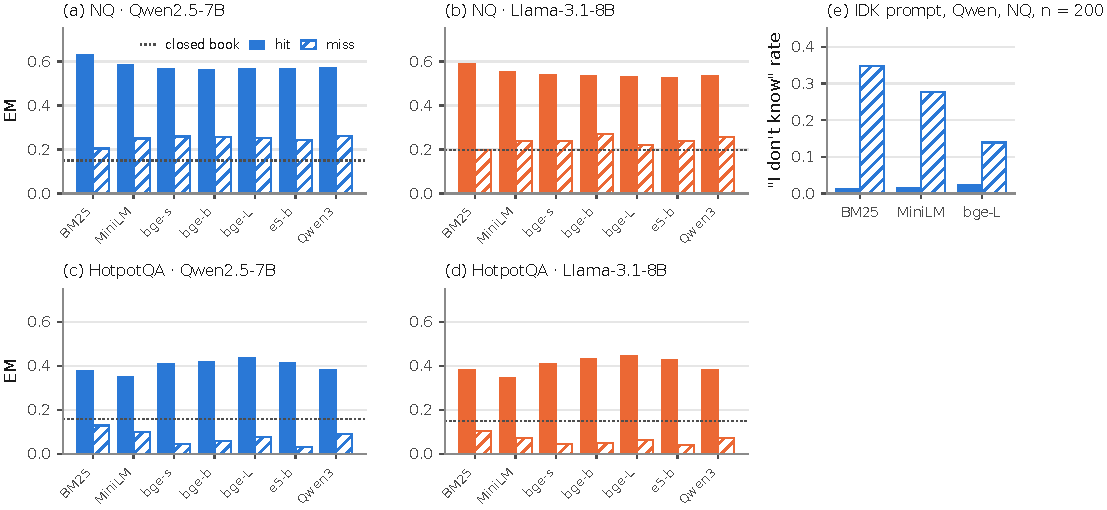
\includegraphics[width=\linewidth]{figs/fig10_error.pdf}
\caption{(a)--(d) Exact match given a hit (solid) and given a miss (hatched) at Hit@5, per reader--dataset cell; dotted line: closed-book EM. (e) Share of ``I don't know'' answers on hits and misses under the abstention prompt A3 (Phase~1, Qwen reader, NQ, 200 queries).}
\label{fig:error}
\end{figure}

\paragraph{Abstention prompt}
A Phase~1 check (Table~\ref{tab:idk}) is consistent with the reading that NQ ``misses'' often still contain usable evidence. When the prompt allowed ``I don't know'' (A3, Appendix~\ref{app:prompts}), the reader abstained mostly on misses: \ev{IDK.miss.R0} of BM25 misses, \ev{IDK.miss.R1} of MiniLM-L6 misses and \ev{IDK.miss.R4} of bge-large misses, against \ev{IDK.hit.R0} to \ev{IDK.hit.R4} of hits. Most misses were still answered. EM under A3 did not differ detectably from the main prompt (\ev{IDK.dem.R0}, \ev{IDK.dem.R1} and \ev{IDK.dem.R4}; $p\ge$ \ev{IDK.p.R4}).

\subsection{Encoder comparisons (RQ2)}\label{sec:res-encoders}
The P2 criterion was met on NQ and not met on HotpotQA (Table~\ref{tab:predictions}). On NQ, neither bge-large nor Qwen3-Embedding-0.6B differed detectably from e5-base-v2 in EM with either reader. On HotpotQA, bge-large gave higher EM than e5-base-v2 with both readers (\ev{P2.qhp.R4}, Holm-adjusted $p$ = \ev{P2.qhp.R4.p}; \ev{P2.lhp.R4}, $p$ = \ev{P2.lhp.R4.p}), in line with its higher Both@5. Qwen3-Embedding-0.6B gave lower EM than e5-base-v2 on HotpotQA (\ev{P2.qhp.R6}, $p$ = \ev{P2.qhp.R6.p}; \ev{P2.lhp.R6}, $p$ = \ev{P2.lhp.R6.p}). The registered pooled model over all four cells (Table~\ref{tab:gee}; \ev{GEE.rows} answers in \ev{GEE.clusters} query clusters) gave odds ratios of \ev{GEE.or.R4} \ev{GEE.ci.R4} for bge-large and \ev{GEE.or.R6} \ev{GEE.ci.R6} for Qwen3-Embedding-0.6B, each against e5-base-v2. This main-effects model assumes the same retriever effect on both datasets, and the data do not support that assumption: the retriever $\times$ dataset terms were jointly significant (Wald $\chi^2_{\ev{V4.gee.int.df}}$ = \ev{V4.gee.int.chi}, $p$ = \ev{V4.gee.int.p}), while retriever $\times$ reader terms were not ($p$ = \ev{V4.gee.rxr.p}). In the interaction model (post hoc), bge-large had an odds ratio of \ev{V4.or.R4.nq} \ev{V4.or.R4.nq.ci} on NQ and \ev{V4.or.R4.hp} \ev{V4.or.R4.hp.ci} on HotpotQA; Qwen3-Embedding-0.6B had \ev{V4.or.R6.nq} \ev{V4.or.R6.nq.ci} and \ev{V4.or.R6.hp} \ev{V4.or.R6.hp.ci}. The small pooled advantage of bge-large thus averages no detected effect on NQ with a gain on HotpotQA, in line with the per-cell tests. Both models mix the two study phases and are secondary.

\begin{table*}[t]
\centering
\small
\caption{GEE logistic models of EM over the four reader--dataset cells: odds ratios against e5-base-v2 [95\% CI].}
\label{tab:gee}
\begin{tabular}{lccc}
\toprule
 & Pooled (main effects) & \multicolumn{2}{c}{With retriever $\times$ dataset interaction} \\
\cmidrule(lr){3-4}
Contrast & both datasets & NQ & HotpotQA \\
\midrule
bge-large vs e5-base-v2 & 1.038 [1.001, 1.076] & 0.981 [0.936, 1.028] & 1.109 [1.049, 1.172] \\
Qwen3-Emb-0.6B vs e5-base-v2 & 0.909 [0.875, 0.943] & 0.952 [0.906, 1.001] & 0.859 [0.811, 0.909] \\
\bottomrule
\end{tabular}
\par\smallskip\parbox{\linewidth}{\footnotesize Pooled: EM $\sim$ retriever + dataset + reader (registered secondary model). Interaction model: EM $\sim$ retriever $\times$ dataset + reader (post hoc). Retriever $\times$ dataset: Wald $\chi^2_{6}$ = 179, $p$ = $5.2\times10^{-36}$; adding retriever $\times$ reader: $\chi^2_{6}$ = 5.0, $p$ = 0.55. Exchangeable working correlation (0.60) within query; 59,570 answers in 4,255 query clusters; empirical (sandwich) standard errors. All models converged without warnings.}
\end{table*}


\subsection{Context choices (RQ3)}\label{sec:res-context}
\paragraph{Number of passages}
Table~\ref{tab:topk} and Fig.~\ref{fig:topk} show EM for $k\in\{1,3,5,10\}$ with Qwen on NQ. One passage gave lower EM than five for every retriever (P4 criterion met; differences from \ev{K1.R0} for BM25 to \ev{K1.R5} for e5-base-v2, all Holm-adjusted $p<0.001$). From five to ten passages, EM rose for six retrievers and stayed flat for e5-base-v2 (\ev{TK.R5.k5} and \ev{TK.R5.k10}). The gap between retrievers shrank with $k$: at $k=10$ all dense encoders gave EM between \ev{TK.R1.k10} and \ev{TK.R4.k10}. In an exploratory check (Table~\ref{tab:transferk}), we matched Hit@$k$ to the $k$ passages the reader saw. The transfer ratio then fell with $k$; for bge-large it was \ev{TKT.R4.k1} \ev{TKT.R4.k1.ci} at $k=1$, \ev{TKT.R4.k3} at $k=3$, \ev{TKT.R4.k5} at $k=5$ and \ev{TKT.R4.k10} \ev{TKT.R4.k10.ci} at $k=10$. The NQ ratios of Section~\ref{sec:res-transfer} therefore describe $k=5$ only. More passages also cost more reading: the mean prompt grew from \ev{TOK.R4_k1} tokens at $k=1$ to \ev{TOK.R4_k5} at $k=5$ and \ev{TOK.R4_k10} at $k=10$ for bge-large. In a second exploratory comparison, bge-large with one passage gave higher EM than BM25 with ten passages (\ev{X41.diff} \ev{X41.ci}; exact McNemar $p$ = \ev{X41.p}, uncorrected).

\begin{figure}[t]
\centering
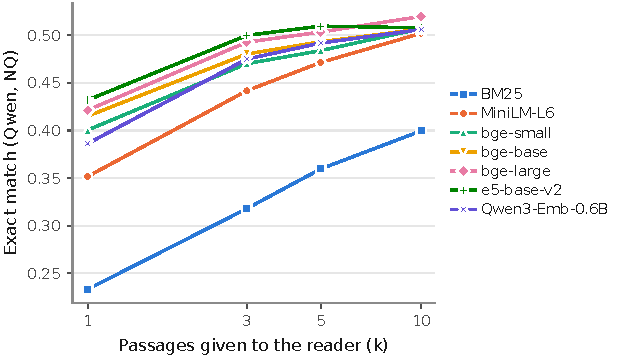
\includegraphics[width=0.85\linewidth]{figs/fig3_topk.pdf}
\caption{Exact match by number of passages $k$, Qwen reader on NQ (2,255 queries).}
\label{fig:topk}
\end{figure}

\paragraph{Passage composition and position}
Table~\ref{tab:mechanism} and Fig.~\ref{fig:mechanism} give the controlled context test on 500 NQ questions. With the gold passage at position 1, four top-ranked non-gold BM25 passages gave EM \ev{MC.M1}, and four random passages gave \ev{MC.MR}: a drop of \ev{P5.abs} (exact McNemar $p$ = \ev{P5.p}; P5 criterion met). Adding four random passages to the gold passage changed EM by no detectable amount: gold at position 1 plus four random passages gave \ev{MC.MR}, and the gold passage alone gave \ev{MC.MG} (difference \ev{V4.mrmg.diff}, 95\% CI \ev{V4.mrmg.ci}; $p$ = \ev{MG.p}). No equivalence margin was registered, so this interval is not evidence that random passages have no effect; it only bounds the effect in this sample of 500 questions. Under the answer-string rule, at least one hard negative contained an answer for \ev{V6.o8.n} of the 500 questions (\ev{V6.o8.share}, Wilson interval \ev{V6.o8.wilson}). On the \ev{V6.o8.clean.n} questions without such a passage, the drop was larger: EM \ev{V6.o8.clean.M1} with hard negatives against \ev{V6.o8.clean.MR} with random passages (\ev{V6.o8.clean.diff}, 95\% CI \ev{V6.o8.clean.ci}; $p$ \ev{V6.o8.clean.p}). On the other questions the two contexts gave \ev{V6.o8.ans.M1} and \ev{V6.o8.ans.MR} (not pre-specified). Answer-bearing hard negatives therefore made the registered P5 effect smaller, not larger. The position of the gold passage among the hard negatives showed no detectable effect (EM \ev{MC.M1}, \ev{MC.M3} and \ev{MC.M5} at positions 1, 3 and 5; all Holm-adjusted $p\ge$ \ev{P6.M1M3.p}; P6 criterion not met).

\begin{figure}[t]
\centering
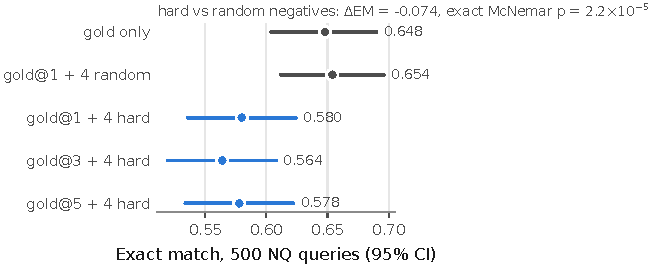
\includegraphics[width=0.75\linewidth]{figs/fig4_mechanism.pdf}
\caption{Exact match for five controlled contexts of five passages (Qwen reader, 500 NQ generation queries) with 95\% bootstrap intervals.}
\label{fig:mechanism}
\end{figure}

\begin{table}[t]
\centering
\small
\caption{Exact match by number of passages $k$ (Qwen reader, NQ, 2,255 queries).}
\label{tab:topk}
\begin{tabular}{lrrrrrr}
\toprule
Retriever & $k{=}1$ & $k{=}3$ & $k{=}5$ & $k{=}10$ & $\Delta_{1-5}$ & $p_\text{Holm}$ \\
\midrule
BM25 & 0.233 & 0.318 & 0.360 & 0.400 & $-$0.126 & $<$0.001 \\
MiniLM-L6 & 0.352 & 0.442 & 0.471 & 0.502 & $-$0.120 & $<$0.001 \\
bge-small & 0.400 & 0.470 & 0.484 & 0.507 & $-$0.083 & $<$0.001 \\
bge-base & 0.415 & 0.480 & 0.493 & 0.506 & $-$0.078 & $<$0.001 \\
bge-large & 0.421 & 0.493 & 0.503 & 0.520 & $-$0.082 & $<$0.001 \\
e5-base-v2 & 0.432 & 0.500 & 0.510 & 0.508 & $-$0.078 & $<$0.001 \\
Qwen3-Emb-0.6B & 0.386 & 0.475 & 0.492 & 0.506 & $-$0.106 & $<$0.001 \\
\bottomrule
\end{tabular}
\par\smallskip\parbox{\linewidth}{\footnotesize Exact McNemar test of $k{=}1$ vs $k{=}5$, Holm over seven retrievers.}
\end{table}

\begin{table}[t]
\centering
\small
\caption{Distraction and position tests (Qwen reader, 500 NQ generation queries).}
\label{tab:mechanism}
\begin{tabular}{lccc}
\toprule
Context (5 passages) & EM [95\% CI] & F1 & AC \\
\midrule
Gold only & 0.648 [0.604, 0.690] & 0.772 & 0.770 \\
Gold@1 + 4 random & 0.654 [0.612, 0.696] & 0.777 & 0.764 \\
Gold@1 + 4 hard & 0.580 [0.536, 0.624] & 0.696 & 0.686 \\
Gold@3 + 4 hard & 0.564 [0.520, 0.608] & 0.684 & 0.672 \\
Gold@5 + 4 hard & 0.578 [0.534, 0.622] & 0.698 & 0.682 \\
\bottomrule
\end{tabular}
\par\smallskip\parbox{\linewidth}{\footnotesize Hard vs random negatives: $\Delta$EM = $-$0.074, exact McNemar $p$ = $2.2\times10^{-{}5}$. Position: no pair differs after Holm.}
\end{table}


\paragraph{Reranking}
The cross-encoder raised the Hit@5 and EM of BM25 and lowered the Hit@5 of e5-base-v2 (Table~\ref{tab:reranker}). On the NQ generation queries, reranking the BM25 top 50 raised Hit@5 by \ev{RR.X0_vs_R0.hit} and EM by \ev{RR.X0_vs_R0.em} (both $p<0.001$). Reranking the e5-base-v2 top 50 changed Hit@5 by \ev{RR.X5_vs_R5.hit} ($p$ = \ev{RR.X5_vs_R5.hit.p}); for EM the change was \ev{RR.X5_vs_R5.em} ($p$ = \ev{RR.X5_vs_R5.em.p}), and no difference was detected. Reranking cost a median of \ev{RR.lat.R0} to \ev{RR.lat.R5}~ms per query on a T4. These results come from one reranker at one depth.

\begin{table}[t]
\centering
\small
\caption{Cross-encoder reranking (bge-reranker-base, top 50) on NQ.}
\label{tab:reranker}
\begin{tabular}{lcccc}
\toprule
System & Hit@5 & nDCG@10 & EM & ms/query \\
\midrule
BM25 & 0.373 & 0.284 & 0.360 & -- \\
BM25 + reranker & 0.658 & 0.542 & 0.456 & 208 \\
e5-base-v2 & 0.817 & 0.665 & 0.510 & -- \\
e5-base-v2 + reranker & 0.742 & 0.601 & 0.494 & 249 \\
\bottomrule
\end{tabular}
\par\smallskip\parbox{\linewidth}{\footnotesize Retrieval on all 3,452 judged queries; EM on the 2,255 generation queries (Qwen). Latency: median per query, 50 pairs, one T4.}
\end{table}


\subsection{Retrieval-stage cost and checks of the setup (RQ4)}\label{sec:res-cost}
\paragraph{Encoding cost}
Table~\ref{tab:cost} gives the measured retrieval-stage cost; reader cost was not part of this measurement. Throughput fell from \ev{E7.tp.R1} passages per second for MiniLM-L6 to \ev{E7.tp.R6} for Qwen3-Embedding-0.6B, a factor of \ev{E7.ratio.R1R6}. e5-base-v2 encoded \ev{E7.ratio.R5R4} times faster than bge-large. The five repetitions varied little (Table~\ref{tab:cost}): no two encoders had overlapping throughput ranges. The closest pair, bge-base and e5-base-v2, share the same architecture size, and bge-base was \ev{V4.tp.R3R5} faster at the median. Query encoding took \ev{E7.lat.R1} to \ev{E7.lat.R6}~ms per query; BM25 took \ev{E7.lat.R0}~ms on the CPU. Fig.~\ref{fig:cost} relates throughput to EM averaged over the four cells. bge-large had the highest average EM (\ev{EMBAR.R4}), bge-base and e5-base-v2 followed at \ev{EMBAR.R5} with \ev{E7.ratio.R5R4} times its throughput, and Qwen3-Embedding-0.6B (\ev{EMBAR.R6}) was both the slowest and below bge-small (\ev{EMBAR.R2}).

\begin{figure}[t]
\centering
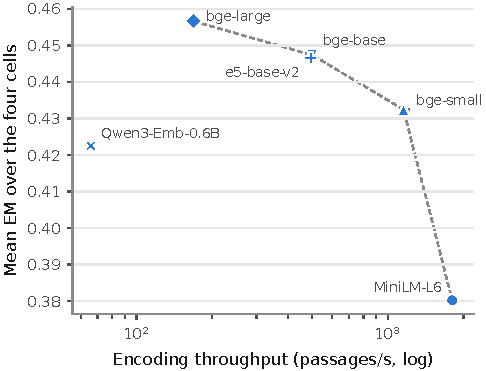
\includegraphics[width=0.6\linewidth]{figs/fig5_cost_quality.pdf}
\caption{Encoding throughput on one T4 GPU (median of five repetitions, log scale) against EM averaged over the four reader--dataset cells. The dashed line joins encoders that no other encoder beats on both axes.}
\label{fig:cost}
\end{figure}

\begin{table}[t]
\centering
\small
\caption{Encoding cost on one Tesla T4, median (range) over five repetitions.}
\label{tab:cost}
\begin{tabular}{lrrcc}
\toprule
Encoder & Params (M) & Dim & Passages/s & Query ms \\
\midrule
MiniLM-L6 & 23 & 384 & 1807 (1768--1863) & 6.0 (6.0--6.1) \\
bge-small & 33 & 384 & 1155 (1136--1207) & 10.3 (10.1--10.3) \\
bge-base & 109 & 768 & 502 (501--503) & 10.0 (9.9--10.1) \\
e5-base-v2 & 109 & 768 & 493 (491--496) & 10.0 (9.9--10.1) \\
bge-large & 335 & 1024 & 168 (168--169) & 18.3 (18.3--18.6) \\
Qwen3-Emb-0.6B & 596 & 1024 & 66 (66--66) & 52.2 (51.8--54.9) \\
\bottomrule
\end{tabular}
\par\smallskip\parbox{\linewidth}{\footnotesize BM25 batch-1 query latency on CPU: 25.7 ms (23.7--27.7).}
\end{table}


\paragraph{CPU deployment} Phase~1 also measured single-query latency with encoding and exact search on the CPU, index size and full sub-corpus encoding time (single measurements). These operational details, with the CPU quality--latency frontier, are in Appendix~\ref{app:deploy}.

\paragraph{Approximate search}
HNSW search kept the exact top five almost unchanged (Table~\ref{tab:hnsw}). At efSearch 128, HNSW returned at least \ev{V5.hnsw.ov5.min128} of the exact top five and \ev{V5.hnsw.ov100.min128} of the exact top 100 (mean shares over all 3,452 judged queries), Hit@5 changed by at most \ev{E6.dhitabs.max}, and the median query latency on the CPU fell from \ev{E6.lat.exact.R1}--\ev{E6.lat.exact.R5}~ms to \ev{E6.lat.ef128.R1}--\ev{E6.lat.ef128.R5}~ms. We did not run the readers on HNSW results, so this check covers retrieval and latency only.

\begin{table*}[t]
\centering
\footnotesize
\caption{Approximate search (HNSW, $M{=}32$, efConstruction 200) against exact search on the NQ sub-corpus, CPU, all 3,452 judged NQ queries.}
\label{tab:hnsw}
\begin{tabular}{lcccccccccc}
\toprule
& \multicolumn{2}{c}{Exact} & \multicolumn{4}{c}{HNSW efSearch 64} & \multicolumn{4}{c}{HNSW efSearch 128} \\ \cmidrule(lr){2-3}\cmidrule(lr){4-7}\cmidrule(lr){8-11} Encoder & Hit@5 & ms & Ov@5 & Ov@100 & Hit@5 & ms & Ov@5 & Ov@100 & Hit@5 & ms \\
\midrule
MiniLM-L6 & 0.673 & 35.9 & 0.998 & 0.946 & 0.672 & 0.50 & 0.999 & 0.984 & 0.673 & 0.84 \\
bge-small & 0.729 & 36.3 & 0.992 & 0.904 & 0.726 & 0.49 & 0.996 & 0.964 & 0.727 & 0.89 \\
e5-base-v2 & 0.817 & 77.7 & 0.995 & 0.915 & 0.815 & 0.80 & 0.997 & 0.970 & 0.817 & 1.45 \\
\bottomrule
\end{tabular}
\par\smallskip\parbox{\linewidth}{\footnotesize Ov@5 / Ov@100: mean share of the exact top 5 / top 100 that HNSW also returns. Hit@5 here is over all judged queries, not the 2,255 generation queries. ms: median batch-1 query latency on 4 vCPUs. No reader was run on HNSW results.}
\end{table*}


\paragraph{Sub-corpus versus full corpus}
On the full NQ corpus the four tested retrievers kept their nDCG@10 order (Kendall's $\tau$ = \ev{E9.tau}; P3 criterion met; Table~\ref{tab:fullcorpus} and Fig.~\ref{fig:fullcorpus}). The dense retrievers lost \ev{E9.dropabs.R2} to \ev{E9.dropabs.R1} in nDCG@10, and BM25 lost almost nothing (\ev{E9.dropabs.R0}). The sub-corpus therefore inflates absolute dense scores but not the order of these four retrievers. The drops also agree with the bias that the construction implies: the sub-corpus keeps BM25's own top-ranked passages for every judged query but not those of the dense encoders, so it favours the dense encoders relative to BM25. Section~\ref{sec:res-full} gives the readers on full-corpus retrieval; HotpotQA was not run on its full corpus.

\begin{figure}[t]
\centering
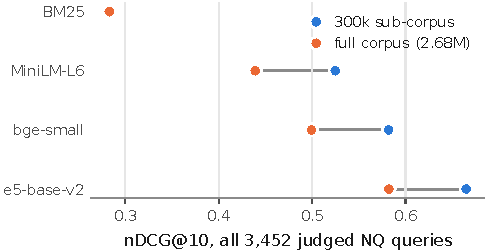
\includegraphics[width=0.6\linewidth]{figs/fig6_full_corpus.pdf}
\caption{nDCG@10 on the 300,000-passage sub-corpus and on the full NQ corpus (all 3,452 judged queries).}
\label{fig:fullcorpus}
\end{figure}

\begin{table}[t]
\centering
\small
\caption{Sub-corpus (300k) vs full NQ corpus (2.68M), all 3,452 judged queries.}
\label{tab:fullcorpus}
\begin{tabular}{lcccc}
\toprule
Retriever & nDCG@10 sub & nDCG@10 full & Hit@5 sub & Hit@5 full \\
\midrule
BM25 & 0.284 & 0.283 & 0.373 & 0.373 \\
MiniLM-L6 & 0.525 & 0.439 & 0.673 & 0.571 \\
bge-small & 0.582 & 0.499 & 0.729 & 0.630 \\
e5-base-v2 & 0.665 & 0.582 & 0.817 & 0.727 \\
\bottomrule
\end{tabular}
\par\smallskip\parbox{\linewidth}{\footnotesize Kendall's $\tau$ between the two orderings = 1.00.}
\end{table}


\subsection{LLM judge validation}\label{sec:res-judge}
The LLM judge agreed poorly with the author's labels (Table~\ref{tab:judge}). Cohen's $\kappa$ was \ev{JA.kappa} \ev{JA.ci}, with raw agreement \ev{JA.raw}. Weighted to the population, the judge labelled \ev{JA.jrate} of answers as supported, against \ev{JA.hrate} for the author, and its precision for the label supported was \ev{JA.prec}. Under the registered rule ($\kappa<0.2$) we excluded the judge's faithfulness labels from all conclusions. For completeness, Table~\ref{tab:judgerates} in the appendix lists the share of answers the judge labelled as supported, and Appendix~\ref{app:judge} gives the judge prompt and the annotation instructions.

\begin{table}[t]
\centering
\small
\caption{Agreement between the author's labels and the LLM judge on 200 stratified items.}
\label{tab:judge}
\begin{tabular}{lcc}
\toprule
& Judge SUPPORTED & Judge NOT\_SUPPORTED \\
\midrule
Human SUPPORTED & 65 & 50 \\
Human NOT\_SUPPORTED & 37 & 48 \\
\bottomrule
\end{tabular}
\par\smallskip\parbox{\linewidth}{\footnotesize Cohen's $\kappa$ = 0.127 [$-$0.006, 0.261]; raw agreement 0.565. Under the pre-registered rule ($\kappa<0.2$) the judge results are excluded from the conclusions.}
\end{table}


\subsection{Summary of the predictions}
Table~\ref{tab:predictions} lists all eight registered criteria. P3, P4, P5, P7 and P8 were met. P1 was not met in one of three new cells (an upper bound of 1.000 or more), P2 was not met in either HotpotQA cell, and P6 was not met. Where a verdict is not confirmatory, the table marks it.

\begin{table*}[t]
\centering
\small
\caption{Registered predictions: whether each stated criterion was met.}
\label{tab:predictions}
\begin{tabular}{lllp{0.55\linewidth}}
\toprule
ID & Scope & Criterion & Evidence \\
\midrule
P1 & NQ, Qwen$^\dagger$ & met & 5 dense-encoder ratios; largest upper bound 0.455 (Qwen3-Emb-0.6B) \\
P1 & NQ, Llama & met & 5 dense-encoder ratios; largest upper bound 0.427 (bge-small) \\
P1 & HotpotQA, Qwen & met & 5 dense-encoder ratios; largest upper bound 0.996 (bge-large) \\
P1 & HotpotQA, Llama & \textbf{not met} & 5 dense-encoder ratios; largest upper bound 1.096 (bge-large) \\
P2 & NQ, Qwen$^\dagger$ & met & bge-large $-$ e5: $-$0.006 ($p_\text{Holm}$ 1.000); Qwen3-Emb-0.6B $-$ e5: $-$0.018 ($p_\text{Holm}$ 0.271) \\
P2 & NQ, Llama & met & bge-large $-$ e5: $-$0.004 ($p_\text{Holm}$ 1.000); Qwen3-Emb-0.6B $-$ e5: $-$0.007 ($p_\text{Holm}$ 1.000) \\
P2 & HotpotQA, Qwen & \textbf{not met} & bge-large $-$ e5: +0.028 ($p_\text{Holm}$ 0.005); Qwen3-Emb-0.6B $-$ e5: $-$0.030 ($p_\text{Holm}$ 0.003) \\
P2 & HotpotQA, Llama & \textbf{not met} & bge-large $-$ e5: +0.022 ($p_\text{Holm}$ 0.040); Qwen3-Emb-0.6B $-$ e5: $-$0.042 ($p_\text{Holm}$ $<$0.001) \\
P3 & NQ, 4 retrievers & met & Kendall's $\tau$ = 1.00 (retrieval only) \\
P4 & NQ, Qwen & met & $k{=}1$ below $k{=}5$ for all 7 retrievers$^\ddagger$; $\Delta$EM $-$0.126 to $-$0.078; all $p_\text{Holm}$ $<$0.001 \\
P5 & NQ, Qwen, 500 q. & met & hard vs random negatives: $\Delta$EM $-$0.074, $p$ $<$0.001 \\
P6 & NQ, Qwen, 500 q. & \textbf{not met} & gold at position 1/3/5: largest $|\Delta$EM$|$ 0.016; smallest $p_\text{Holm}$ 0.94 \\
\bottomrule
\end{tabular}
\par\smallskip\parbox{\linewidth}{\footnotesize P1: every reportable EM transfer ratio of a dense encoder has an upper 95\% bound below 1 (unrounded; a bound of exactly 1.000 does not meet it). P2: no Holm-significant EM gain of bge-large or Qwen3-Emb-0.6B over e5-base-v2. P3: the full corpus keeps the nDCG@10 ordering. P4: EM at $k{=}1$ below $k{=}5$. P5: hard negatives lower EM. P6: gold position changes EM. $^\dagger$Not confirmatory: observed in Phase 1, before registration. $^\ddagger$Confirmatory for bge-small, bge-base, e5-base-v2 and Qwen3-Emb-0.6B only. The v0.3 analysis code also counted BM25 in the NQ P1 checks (six ratios); the registered criterion covers dense encoders, and the verdict is the same either way.}
\end{table*}


\section{Discussion}\label{sec:discussion}

\subsection{What the transfer ratio shows}
On single-hop NQ, a retrieval gain of a dense encoder over a small encoder reached the answer at a rate of \ev{T.lnq.R4} to \ev{T.lnq.R3} EM points per Hit@5 point, with both readers. Three observations within our setup are consistent with this. (i) The readers fell well short of their gold-passage bound even with good retrieval, so part of the loss lies in reading, not retrieval. (ii) EM given a miss stayed far above closed-book EM. The NQ relevance labels are sparse, so many ``misses'' likely still contained an answer-bearing passage that was not labelled gold, or the reader knew the answer. Hit@5 may therefore overstate the difference between encoders that matters for the reader. (iii) EM given a hit fell slightly as encoders improved, which suggests that the questions that a better encoder newly solves at the retrieval stage are harder to answer. This last point is a hypothesis; we did not test which questions changed status.

On multi-hop HotpotQA, Hit@5 saturated while Both@5 did not. In the baseline-conditioned decomposition, between \ev{DS.hp.min} and \ev{DS.hp.max} of the transfer came from higher EM given a hit (\ev{V4.sym.hp.min}--\ev{V4.sym.hp.max} in the symmetric form), and the EM ranking of retrievers followed Both@5 exactly. Both are descriptions of the data, not causal attributions. A reasonable reading is that, for bridge questions, the second supporting passage carries the answer, and Hit@5 does not count it. A post hoc check supports this reading: with Both@5 as the denominator, the HotpotQA ratios fell to \ev{V4.both.hp.min}--\ev{V4.both.hp.max}, much closer to the NQ range. The large Hit@5-based ratios on HotpotQA therefore largely reflect the denominator: the retrieval gain that matters is larger than Hit@5 shows. The comparison questions, where both entities are named in the question, were close to their gold bound for every dense encoder. Teams that build multi-hop systems may therefore prefer to measure retrieval with a metric that requires all needed evidence.

Measured with Hit@5, the two datasets thus support different conclusions about the same encoders. A team that judges encoders by single-hop retrieval benchmarks may overrate the answer value of the strongest ones. A team with multi-hop questions may underrate it if it uses Hit@k.

\subsection{Comparison with earlier work}
Our NQ results agree with reports that retrieval gains do not carry over fully to answers \citep{salemi2024erag,mathur2026policy,ghosh2026evidence} and with the falling recall conversion rate reported by \citet{peng2026neocorrag}. They do not contradict the strong correlations reported by \citet{samuel2026beyond}: the EM ranking of retrievers followed their Hit@5 ranking closely in every cell (Spearman $\rho$ between \ev{RHO.lnq} and \ev{RHO.qnq}). Correlation concerns the order of systems; the transfer ratio concerns the size of the gain. A metric can rank encoders correctly and still overstate how much answers improve.

The context experiment agrees with earlier findings on distraction. Top-ranked non-gold passages lowered EM compared with random passages \citep{cuconasu2024power,amiraz2025distracting,repantis2026competition}, and adding random passages to the gold passage changed EM by no detectable amount. Gold position showed no detectable effect among five passages, in line with \citet{cuconasu2025positional}; with five short passages our setting is far from the long contexts in which position effects were originally shown \citep{liu2024lost}. The near-identical retrieval results of exact and approximate search agree with \citet{leto2024toward}, who also measured answers; we measured retrieval only.

\subsection{Practical implications}
Within our setup, the choice of encoder mattered less for answers than for retrieval, while its cost differed by more than an order of magnitude. For single-hop questions, a base-size encoder such as e5-base-v2 or bge-base gave answers that no larger encoder improved detectably, while encoding \ev{E7.ratio.R5R4} times faster than bge-large. For multi-hop questions, bge-large gave a small but detectable gain. Qwen3-Embedding-0.6B was the most expensive encoder and gave lower EM than e5-base-v2 on HotpotQA; its instruction and length settings may not suit this task, and we did not tune them. Retrieving ten passages instead of five raised EM for most retrievers and narrowed their differences, which is another lever when the reader's context allows it, although it nearly doubles the prompt the reader must process. A cross-encoder helped the weak BM25 retrieval stage but not a strong dense one. Approximate search returned nearly the same top five passages as exact search at a small fraction of the latency; we did not measure its effect on answers.

\subsection{Alternative explanations}
Several features of the design could produce low NQ transfer without a property of the encoders. EM undercounts correct answers \citep{kamalloo2023}; the F1 and containment ratios were higher but showed the same contrast between datasets. The sub-corpus inflates dense retrieval scores, but the full-corpus check kept the order of four retrievers, and the inflation was similar for the three dense encoders tested (\ev{E9.dropabs.R2} to \ev{E9.dropabs.R1} in nDCG@10). The construction favours the dense encoders relative to BM25, so the comparisons that involve BM25 depend most on it. The readers were 4-bit quantised 7--8B models with one prompt; stronger readers may convert hits into answers at a different rate. The baseline encoder also matters: $T(R)$ against MiniLM-L6 measures gains above a fairly strong small encoder. Against BM25 the NQ ratios were higher (\ev{V4.b0.nq.min}--\ev{V4.b0.nq.max}), and the contrast between datasets held for four of the five dense encoders but reversed for Qwen3-Embedding-0.6B (Table~\ref{tab:altbase}). The ratio therefore describes a pair of retrievers, not a single encoder, and the dataset contrast is clearest against the small dense baseline.

\section{Limitations}\label{sec:limits}

\paragraph{Scope}
The study covers two English Wikipedia question-answering datasets, six open encoders up to 0.6B parameters, two 4-bit 7--8B readers, one prompt and $k=5$ for the registered transfer ratios; the exploratory ratios at other $k$ show that the size of the ratio depends on how many passages the reader sees. Results may differ for other domains, longer answers, larger or proprietary readers, other prompts or agentic pipelines. All timings come from one GPU type (Tesla T4) and one CPU configuration.

\paragraph{Corpus and labels}
Except for Phase~3, retrieval ran on 300,000-passage sub-corpora that contain every gold passage and favour the dense encoders relative to BM25. Phase~3 tested the NQ ratios on the full corpus for BM25, MiniLM-L6, bge-small and e5-base-v2 only; bge-base, bge-large, Qwen3-Embedding-0.6B and all of HotpotQA rest on the sub-corpus. NQ relevance labels are sparse. The answer-string check is lexical; the human audit agreed with it on most items but covers 100 misses of one encoder on the sub-corpus, labelled by one annotator, the author. The joined NQ set covers \ev{N.nq.joined} of \ev{N.nq.judged} judged queries and may differ in difficulty from the excluded queries. A Phase~1 check found Hit@5 differences between joined and unjoined queries from \ev{D1B.min} to \ev{D1B.max} across the seven retrievers, and every 95\% interval included zero.

\paragraph{Metrics and statistics}
EM is strict. We report F1 and answer containment; correctness was judged by hand only for the 100 audited misses. The transfer ratio is a ratio of means and becomes unstable when the retrieval gain is small; our reporting rule removes the worst cases, but the bge-small intervals on NQ still include zero. The ratio depends on the baseline encoder, and the share of the gain assigned to conditional EM depends on how the decomposition is ordered (Tables~\ref{tab:altbase} and~\ref{tab:share}). The decomposition, the query-level accounting, the Both@5 ranking and ratios, the BM25 baseline and the GEE interaction model are post hoc. The accounting groups are defined by retrieval outcomes, so they locate the EM difference but do not explain it. The registered pooled GEE model assumed one retriever effect across datasets, which the interaction test did not support. Answer quality under approximate search was not measured. Multiplicity is controlled within each family, not across all tests in the paper. Bootstrap intervals, F1, answer containment and the pooled model were checked by a rerun on a second computer, not by an independent implementation.

\paragraph{Context experiment}
The hard negatives are top-ranked BM25 passages without a gold label, and a third of the questions had at least one that contained an answer string. Excluding those questions made the measured drop larger, so this does not weaken P5, but the subset analysis is a sensitivity check on 333 questions. The experiment used one reader and 500 questions. The random-passage control found no detected difference from the gold passage alone; it does not establish equivalence.

\paragraph{Judge and annotation}
The LLM judge was validated against one annotator, the author. With $\kappa$ = \ev{JA.kappa} the judge was excluded under the registered rule, so this limitation does not affect the conclusions, but no faithfulness result is reported.

\paragraph{Three study phases}
The predictions were registered in dated, version-controlled design documents in our own repository, not in a public registry. The Qwen--NQ cell and part of the $k$ ablation were run before the predictions were registered, and the software image changed between Phases~1 and~2. P7 and P8 were registered after the sub-corpus results were known; they test whether those results replicate, not a new hypothesis. Within-cell comparisons share one environment. For comparisons across phases, \ev{CS.same} of \ev{CS.n} identical prompts gave identical outputs.

\section{Conclusion}\label{sec:conclusion}

We measured how much of a retrieval gain reaches the answer when a RAG system swaps one open embedding model for another. On single-hop NQ, between \ev{T.lnq.R4} and \ev{T.lnq.R3} EM points followed each Hit@5 point that a dense encoder gained over MiniLM-L6, for both readers (RQ1); against BM25 the ratios were \ev{V4.b0.nq.min} to \ev{V4.b0.nq.max}. On multi-hop HotpotQA the Hit@5-based ratio was larger; in a post hoc decomposition, \ev{DS.hp.min} to \ev{DS.hp.max} of it came from higher EM given a hit, in line with better encoders retrieving the second supporting passage more often, which Hit@5 does not count; with Both@5 as the denominator, the HotpotQA ratios were \ev{V4.both.hp.min} to \ev{V4.both.hp.max}. Among dense encoders, bge-large gave a small EM gain over e5-base-v2 on HotpotQA and none detectable on NQ, and Qwen3-Embedding-0.6B gave lower EM on HotpotQA (RQ2). Top-ranked non-gold passages lowered EM, gold position did not change it detectably, a reranker helped only the weak BM25 retrieval stage, and ten passages narrowed the gaps between retrievers (RQ3). Encoding throughput differed \ev{E7.ratio.R1R6}-fold, while approximate search returned nearly the same top passages and the four retrievers tested on the full NQ corpus kept their order (RQ4).

Within this setup, retrieval gains overstated answer gains on single-hop questions, and on multi-hop questions once retrieval was scored by Both@5; Hit@5 hid much of the multi-hop retrieval gain. We recommend that RAG studies report answer gains next to retrieval gains, with paired intervals and the baseline stated, and use retrieval metrics that require all evidence a question needs. Future work should test larger readers and other domains, run the readers on the full corpus and on approximate-search results, and replace EM with validated human or model judgements.

\section*{Ethics statement}
\paragraph{Data and licences} We used public resources under their licences, as listed on their Hugging Face cards (accessed 17 October 2026): the BEIR versions of Natural Questions and HotpotQA (CC BY-SA 4.0), NQ-open (CC BY-SA 3.0) and HotpotQA (CC BY-SA 4.0). The encoders are released under Apache-2.0 (all-MiniLM-L6-v2, Qwen3-Embedding-0.6B) or MIT (bge, e5 and bge-reranker-base); Qwen2.5-7B-Instruct-AWQ and Mistral-7B-Instruct-v0.3 under Apache-2.0; and the Llama-3.1-8B-Instruct AWQ build under the Llama 3.1 Community License. We used each for research evaluation. The questions are public benchmark questions over Wikipedia; we collected no personal data.

\paragraph{Human annotation} The 200 judge-validation items were labelled by one member of the study team, with the same instructions the judge received and without seeing its verdicts. The same person labelled the 100 audited retrieval misses, blinded as described in Section~\ref{sec:res-decomp}. No external participants were involved.

\paragraph{Risks} The study compares existing models and creates no new model. Readers may over-generalise the comparison to other readers, corpora or languages; we scope each claim to the tested setup. The excluded LLM judge should not be used as evidence that a system gives faithful answers.

\paragraph{Compute} All experiments ran on free Kaggle sessions with Tesla T4 GPUs; the study had no monetary cost.

\section*{Data and code availability}
All code, prompts, design documents with their registration dates, raw reader outputs, scored answers and analysis scripts are kept in one version-controlled repository. To preserve double-anonymised review, its link is given to the editor on the separate title page; an archived copy with a DOI will be deposited on acceptance. The datasets and models are public under their own licences; the exact revisions are listed in Appendix~\ref{app:repro}. Every number in this paper is generated by script from the committed outputs, including the post hoc analyses, whose scripts are in the same repository.

\section*{Declaration of generative AI and AI-assisted technologies in the manuscript preparation process}
During the preparation of this work the author used Claude (Anthropic) to write and test analysis and experiment code, to check references against bibliographic databases, and to draft and edit text. After using this tool, the author reviewed and edited the content as needed and takes full responsibility for the content of the published article. Figures and tables were generated by scripts from the experimental data.


\bibliographystyle{cas-model2-names}
\bibliography{references}

\appendix
\section{Reader prompts}\label{app:prompts}
The prompts below are copied from the code that ran the readers (\texttt{src/generation/prompts.py}). Every generation record stores a hash of the system prompt; all \ev{IC.n} scored answers carry the hash of the prompt printed here (A1: \ev{N.gen.A1}, A2: \ev{N.gen.A2}, A3: \ev{N.gen.A3} records). Each prompt was rendered with the reader's own chat template.

\paragraph{User message (A1 and A3)} Passages appear in rank order, each as ``[$i$] title'', a line break and the passage text, separated by blank lines:
\begin{quote}\small\ttfamily
Passages:\\
{[}1{]} \{title 1\}\\
\{text 1\}\\[0.5ex]
{[}2{]} \{title 2\}\\
\{text 2\}\\
\ldots\\[0.5ex]
Question: \{question\}\\
Answer:
\end{quote}

\paragraph{A1 (main prompt, with passages)} System: \emph{``You are a question answering assistant. Answer the question using the passages provided. If the passages do not contain the answer, give your best short answer anyway. Reply with the answer only, as a short phrase of a few words, with no explanation.''}

\paragraph{A2 (closed book)} System: \emph{``You are a question answering assistant. Reply with the answer only, as a short phrase of a few words, with no explanation.''} User: \texttt{Question: \{question\}} followed by a line break and \texttt{Answer:}.

\paragraph{A3 (abstention check, Phase~1 only)} System: \emph{``You are a question answering assistant. Answer the question using only the passages provided. If the passages do not contain the answer, reply exactly: I don't know. Otherwise reply with the answer only, as a short phrase of a few words, with no explanation.''} User message as for A1.

The gold-passage condition uses A1 with the gold passages only.

\section{Judge prompt and annotation instructions}\label{app:judge}
The LLM judge (Mistral-7B-Instruct-v0.3, greedy decoding, at most 8 new tokens) received one user message:

\begin{quote}\small
\emph{You will be given PASSAGES, a QUESTION, and an ANSWER. Decide whether the ANSWER is fully supported by the PASSAGES. An answer is SUPPORTED only if the passages state it or directly imply it. Do not use outside knowledge. Do not judge whether the answer is true in the real world.}\\
\emph{PASSAGES:} [the same five passages the reader saw, formatted as in Appendix~\ref{app:prompts}]\\
\emph{QUESTION:} \{question\} \quad \emph{ANSWER:} \{answer\}\\
\emph{Reply with exactly one word: SUPPORTED or NOT\_SUPPORTED.}
\end{quote}

The verdict was the label SUPPORTED or NOT\_SUPPORTED found at the start of the output; there were no parse failures. The human annotator saw the same text, without the judge's verdict, plus the instruction: \emph{``Label each item SUPPORTED or NOT\_SUPPORTED. If unsure, choose NOT\_SUPPORTED and add a note.''} The 200 items were drawn by a seeded, stratified sampler that over-represents NOT\_SUPPORTED verdicts; population-weighted statistics use the inverse inclusion probabilities.

\section{Models, data and software}\label{app:repro}
\begin{table}[h]
\centering
\small
\caption{Pinned revisions (leading eight characters of the Hugging Face commit).}
\label{tab:revisions}
\begin{tabular}{ll}
\toprule
Resource & Revision \\
\midrule
sentence-transformers/all-MiniLM-L6-v2 & 1110a243 \\
BAAI/bge-small-en-v1.5 & 5c38ec7c \\
BAAI/bge-base-en-v1.5 & a5beb1e3 \\
BAAI/bge-large-en-v1.5 & d4aa6901 \\
intfloat/e5-base-v2 & f52bf8ec \\
Qwen/Qwen3-Embedding-0.6B & 97b0c614 \\
Qwen/Qwen2.5-7B-Instruct-AWQ & b2503754 \\
hugging-quants/Meta-Llama-3.1-8B-Instruct-AWQ-INT4 & db1f81ad \\
BAAI/bge-reranker-base & 2cfc18c9 \\
mistralai/Mistral-7B-Instruct-v0.3 (judge) & c170c708 \\
BeIR/nq & b7253e6c \\
BeIR/nq-qrels & 519acd4e \\
google-research-datasets/nq\_open & 5dd9790a \\
BeIR/hotpotqa & a7e8bab2 \\
BeIR/hotpotqa-qrels & b15429e9 \\
hotpotqa/hotpot\_qa & 1908d6af \\
\bottomrule
\end{tabular}
\end{table}

Retrieval used bm25s 0.3.11 and faiss-cpu 1.15.1; readers used vLLM 0.30.0 with PyTorch 2.13.0 (CUDA 13.0) and Transformers 5.17.0, in half precision with a maximum model length of 4,096 tokens. Table~\ref{tab:env} lists the software of every session.

\begin{table*}[t]
\centering
\footnotesize
\caption{Software in each Kaggle session, read from the environment log that each session wrote.}
\label{tab:env}
\begin{tabular}{lllllll}
\toprule
Session & Python & PyTorch & CUDA & Transformers & vLLM & NumPy \\
\midrule
Phase 1, NQ retrieval and encoding & 3.12.13 & 2.10.0 & 12.8 & 5.0.0 & -- & 2.0.2 \\
Phase 1, Qwen reader (NQ) & 3.12.13 & 2.13.0 & 13.0 & 5.17.0 & 0.30.0 & 2.0.2 \\
Phase 1, judge and CPU cost & 3.12.13 & 2.13.0 & 13.0 & 5.17.0 & 0.30.0 & 2.0.2 \\
Phase 2, HotpotQA retrieval & 3.13.15 & 2.11.0 & 12.8 & 5.0.0 & -- & 2.1.3 \\
Phase 2, HotpotQA readers & 3.13.15 & 2.13.0 & 13.0 & 5.17.0 & 0.30.0 & 2.1.3 \\
Phase 2, Llama reader (NQ), top-$k$ & 3.13.15 & 2.13.0 & 13.0 & 5.17.0 & 0.30.0 & 2.1.3 \\
Phase 2, E5, E6, E7, E9, E12 & 3.13.15 & 2.13.0 & 13.0 & 5.17.0 & 0.30.0 & 2.1.3 \\
Phase 3, full-corpus NQ readers (S5) & 3.13.15 & 2.13.0 & 13.0 & 5.17.0 & 0.30.0 & 2.1.3 \\
\bottomrule
\end{tabular}
\par\smallskip\parbox{\linewidth}{\footnotesize All sessions: bm25s 0.3.11, faiss 1.15.1, sentence-transformers 5.4.1, 4 vCPUs, 31.3 GiB memory, 2 Tesla T4 (14,911 MiB each).}
\end{table*}

\begin{table*}[t]
\centering
\footnotesize
\setlength{\tabcolsep}{3.5pt}
\caption{Retrievers. Dense encoders truncate at 256 tokens, run in half precision and use exact inner-product search over normalised vectors.}
\label{tab:models}
\begin{tabular}{lllrrl}
\toprule
Retriever & Model & Revision & Params (M) & Dim & Query prefix \\
\midrule
BM25 & bm25s 0.3.11, Lucene variant, $k_1=1.2$, $b=0.75$ & -- & -- & -- & -- \\
MiniLM-L6 & sentence-transformers/all-MiniLM-L6-v2 & 1110a243 & 23 & 384 & none \\
bge-small & BAAI/bge-small-en-v1.5 & 5c38ec7c & 33 & 384 & BGE instruction \\
bge-base & BAAI/bge-base-en-v1.5 & a5beb1e3 & 109 & 768 & BGE instruction \\
bge-large & BAAI/bge-large-en-v1.5 & d4aa6901 & 335 & 1024 & BGE instruction \\
e5-base-v2 & intfloat/e5-base-v2 & f52bf8ec & 109 & 768 & ``query: '' \\
Qwen3-Emb-0.6B & Qwen/Qwen3-Embedding-0.6B & 97b0c614 & 596 & 1024 & task instruction \\
\bottomrule
\end{tabular}
\par\smallskip\parbox{\linewidth}{\footnotesize BGE instruction: \emph{Represent this sentence for searching relevant passages:}. e5-base-v2 also prefixes passages with ``passage: ''. Qwen3-Embedding uses a task instruction per dataset.}
\end{table*}

\begin{table}[t]
\centering
\small
\caption{Data and sub-corpora.}
\label{tab:data}
\begin{tabular}{lll}
\toprule
Item & NQ & HotpotQA \\
\midrule
Full corpus (passages) & 2,681,468 & 5,233,329 \\
Judged test queries & 3,452 & 7,405 \\
Queries joined to reference answers & 2,255 & 7,405 \\
Generation queries & 2,255 & 2,000 (1,616 bridge, 384 comparison) \\
Gold passages per judged query & 1.22 (range 1--4) & 2 (every query) \\
Distinct gold passages in the corpus & 4,201 & 13,783 (shared across queries) \\
Sub-corpus size & 300,000 & 300,000 \\
\quad gold passages & 4,201 & 13,783 \\
\quad top-$d$ BM25 passages, non-gold (depth $d$) & 127,791 ($d$ = 42) & 118,726 ($d$ = 19) \\
\quad random passages & 168,008 & 167,491 \\
Reference answers & NQ-open (validation) & HotpotQA fullwiki (validation) \\
\bottomrule
\end{tabular}
\par\smallskip\parbox{\linewidth}{\footnotesize Corpus sizes as distributed by BEIR. Joins: NQ by normalised question text, HotpotQA by question id. Each HotpotQA query has exactly two distinct gold passages; 14,810 gold references point to 13,783 distinct passages because some passages support several questions. Both@5 requires both gold passages of the query in the top five.}
\end{table}


\section{Design documents}\label{app:prereg}
The design document and its addenda are dated and versioned in the study repository. Each was written before the stage it governs.
\begin{itemize}
\item \textbf{v0.2 (26 September 2026).} Research questions, retrievers, reader, judge, metrics, statistical tests, the transfer-ratio reporting rule and the pilot plan.
\item \textbf{v0.2.1--v0.2.2 (26 September 2026).} Follow-up rules (abstention-prompt check, judge fallback, GPU stopping rules) and the change of the NQ join gate (deviation~1).
\item \textbf{v0.2.3 (27 September 2026).} Pilot verification; the sub-corpus membership rule for all judged queries; dropping the RAGAS cross-check.
\item \textbf{v0.2.4 (27--29 September 2026).} Execution records of Phase~1, the failed initial reading session, the cost-estimate error and the cut dimension ablation.
\item \textbf{v0.3 (12 October 2026).} Phase~2 experiments E1--E12 and predictions P1--P6, written before any Phase~2 run.
\item \textbf{v0.3.1 (12 and 14 October 2026).} The Python~3.13 image change and the torchaudio fix.
\item \textbf{v0.3.2 (15 October 2026).} Implementation of E5, E6, E7, E9 and E12 before the session that ran them, including the reduced scope of E6.
\item \textbf{v0.4 (17 October 2026).} Phase~3: readers on full-corpus NQ retrieval, predictions P7 and P8, the answer-string checks and the human audit of misses, written and committed before the Phase~3 session.
\end{itemize}
Pilot numbers were used only for planning and are not reported as results.

\section{Retrieval-stage cost on a CPU}\label{app:deploy}
Phase~1 also measured the cost of serving queries without a GPU (Table~\ref{tab:deploy}; single measurements). Encoding the 300,000-passage sub-corpus on the T4 took \ev{DC.encode_gpu_s.R1}~s with MiniLM-L6, \ev{DC.encode_gpu_s.R5}~s with e5-base-v2, \ev{DC.encode_gpu_s.R4}~s with bge-large and \ev{DC.encode_gpu_s.R6}~s with Qwen3-Embedding-0.6B. On the CPU alone, one query (encoding plus exact search) took \ev{DC.qcpu.query_ms_cpu.R0}~ms with BM25, \ev{DC.qcpu.query_ms_cpu.R1}~ms with MiniLM-L6, \ev{DC.qcpu.query_ms_cpu.R5}~ms with e5-base-v2, \ev{DC.qcpu.query_ms_cpu.R4}~ms with bge-large and \ev{DC.qcpu.query_ms_cpu.R6}~ms with Qwen3-Embedding-0.6B. The flat index took \ev{DC.index_mb.R1}, \ev{DC.index_mb.R5} and \ev{DC.index_mb.R4}~MB at 384, 768 and 1,024 dimensions. Fig.~\ref{fig:pareto} places each retriever by CPU latency and EM in every cell. bge-large and Qwen3-Embedding-0.6B were dominated on NQ for both readers: a cheaper retriever gave at least the same EM. On HotpotQA, bge-large was on the frontier with both readers, and its step over the next retriever was significant only with Qwen. Fig.~\ref{fig:latency} in the appendix gives the same view for NQ nDCG@10. In an exploratory check that treats costs within 5\% as equal, only one frontier changed, on both cost axes: with Qwen on NQ, bge-base left the frontier, because its cost is within 5\% of e5-base-v2 and its EM is lower.

\begin{figure}[t]
\centering
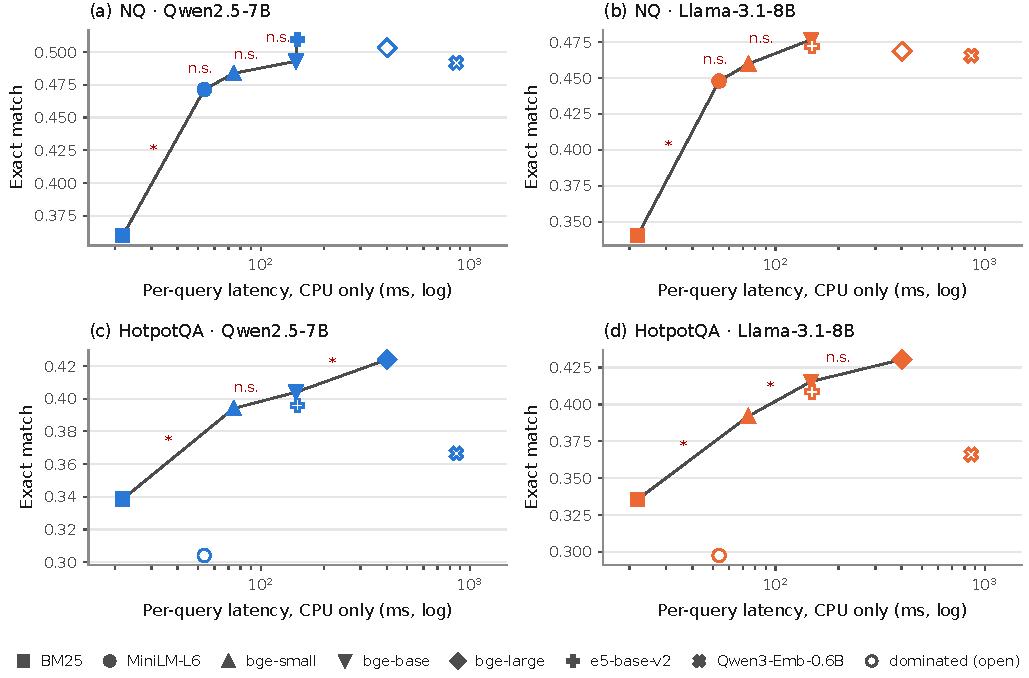
\includegraphics[width=\linewidth]{figs/fig11_pareto.pdf}
\caption{Exact match against per-query latency with query encoding and exact search on the CPU (Phase~1 cost measurements, log scale). The line joins retrievers that no other retriever beats on both axes; open markers are dominated. Step labels: $^{*}$ EM difference significant after Holm correction over the 21 pairs of the cell; n.s. not significant.}
\label{fig:pareto}
\end{figure}

\begin{table*}[t]
\centering
\footnotesize
\setlength{\tabcolsep}{3.5pt}
\caption{Deployment cost measured in Phase 1 (single measurements; one Tesla T4 and four virtual CPUs).}
\label{tab:deploy}
\begin{tabular}{lrrrrrrrr}
\toprule
Retriever & Enc.\ 300k (s) & GPU MiB & CPU pass./s & Q-enc GPU & Q-enc CPU & Search & Query CPU & Index MB \\
\midrule
BM25 & -- & -- & -- & -- & -- & 21.9 & 21.9 & -- \\
MiniLM-L6 & 158 & 352 & 38.7 & 5.6 & 14.3 & 39.3 & 53.7 & 439 \\
bge-small & 250 & 374 & 20.0 & 9.7 & 35.3 & 38.8 & 74.1 & 439 \\
bge-base & 584 & 818 & 6.4 & 9.6 & 66.5 & 81.2 & 147.7 & 879 \\
bge-large & 1,753 & 1,427 & 1.9 & 17.4 & 259.4 & 143.1 & 402.5 & 1,172 \\
e5-base-v2 & 592 & 818 & 6.2 & 9.6 & 67.8 & 81.5 & 149.3 & 879 \\
Qwen3-Emb-0.6B & 4,431 & 7,548 & 0.3 & 46.9 & 719.7 & 142.0 & 861.7 & 1,172 \\
\bottomrule
\end{tabular}
\par\smallskip\parbox{\linewidth}{\footnotesize Enc.\ 300k: T4 wall time to encode the 300,000-passage sub-corpus. Q-enc: batch-1 query encoding (ms, median). Search: batch-1 exact inner-product search on the CPU (ms, median). Query CPU: query encoding plus search, all on the CPU. Index: flat float32 FAISS index. Encoding throughput repeated five times in Phase 2 is in Table~\ref{tab:cost}.}
\end{table*}



\section{Additional tables}\label{app:tables}
Table~\ref{tab:ci} gives the bootstrap intervals for Table~\ref{tab:main}. Table~\ref{tab:transferalt} repeats the transfer ratios with token F1 and answer containment. Table~\ref{tab:decomp} gives EM given a hit and given a miss, which enter Eq.~\ref{eq:decomp}. Table~\ref{tab:idk} gives the abstention-prompt check, Table~\ref{tab:transferk} the exploratory transfer ratios at each $k$, Table~\ref{tab:pairwise} all pairwise EM tests, and Table~\ref{tab:judgerates} the excluded judge labels. Table~\ref{tab:components} gives the three decomposition terms with intervals, Table~\ref{tab:transdetail} the query-level transitions for two encoders, Table~\ref{tab:share} the HotpotQA shares under both orderings, and Table~\ref{tab:altbase} the ratios against BM25 and with Both@5.

\begin{table*}[t]
\centering
\small
\caption{95\% percentile bootstrap intervals (10,000 resamples over queries, seed 0) for the values in Table~\ref{tab:main}. Upper block: exact match per reader and dataset. Lower block: retrieval metrics, which do not depend on the reader.}
\label{tab:ci}
\begin{tabular}{lcccc}
\toprule
Condition & NQ Qwen & NQ Llama & HotpotQA Qwen & HotpotQA Llama \\
\midrule
BM25 & [0.340, 0.380] & [0.321, 0.360] & [0.318, 0.359] & [0.315, 0.356] \\
MiniLM-L6 & [0.451, 0.492] & [0.427, 0.469] & [0.284, 0.325] & [0.278, 0.318] \\
bge-small & [0.463, 0.505] & [0.439, 0.481] & [0.372, 0.415] & [0.370, 0.413] \\
bge-base & [0.473, 0.513] & [0.456, 0.497] & [0.383, 0.426] & [0.394, 0.438] \\
bge-large & [0.482, 0.524] & [0.448, 0.489] & [0.402, 0.446] & [0.408, 0.453] \\
e5-base-v2 & [0.489, 0.530] & [0.452, 0.493] & [0.374, 0.417] & [0.387, 0.430] \\
Qwen3-Emb-0.6B & [0.471, 0.512] & [0.445, 0.487] & [0.345, 0.388] & [0.345, 0.388] \\
Closed book & [0.135, 0.164] & [0.180, 0.213] & [0.143, 0.174] & [0.133, 0.165] \\
Gold passages & [0.633, 0.673] & [0.593, 0.633] & [0.607, 0.649] & [0.602, 0.645] \\
\midrule
Retrieval & NQ Hit@5 & & HotpotQA Hit@5 & HotpotQA Both@5 \\
\midrule
BM25 & [0.343, 0.383] & & [0.816, 0.849] & [0.244, 0.283] \\
MiniLM-L6 & [0.645, 0.683] & & [0.799, 0.834] & [0.212, 0.248] \\
bge-small & [0.710, 0.747] & & [0.944, 0.963] & [0.519, 0.563] \\
bge-base & [0.753, 0.788] & & [0.949, 0.967] & [0.550, 0.594] \\
bge-large & [0.779, 0.812] & & [0.952, 0.969] & [0.599, 0.642] \\
e5-base-v2 & [0.800, 0.832] & & [0.941, 0.960] & [0.522, 0.567] \\
Qwen3-Emb-0.6B & [0.726, 0.762] & & [0.934, 0.955] & [0.422, 0.467] \\
\bottomrule
\end{tabular}
\end{table*}

\begin{table*}[t]
\centering
\footnotesize
\caption{Components of the EM gain over MiniLM-L6 (Eq.~\ref{eq:decomp} multiplied by $\Delta\bar h$), with 95\% bootstrap intervals. Post hoc, descriptive.}
\label{tab:components}
\begin{tabular}{lcccc}
\toprule
Encoder & $\Delta$EM & Hit prevalence & EM among hits & EM among misses \\
\midrule
\multicolumn{5}{l}{\emph{NQ Qwen}} \\
bge-small & +0.012 & +0.022 [0.015, 0.029] & \ensuremath{-}0.012 [\ensuremath{-}0.026, 0.003] & +0.003 [\ensuremath{-}0.007, 0.012] \\
bge-base & +0.022 & +0.036 [0.028, 0.043] & \ensuremath{-}0.016 [\ensuremath{-}0.031, 0.000] & +0.002 [\ensuremath{-}0.007, 0.011] \\
bge-large & +0.032 & +0.044 [0.036, 0.052] & \ensuremath{-}0.013 [\ensuremath{-}0.029, 0.004] & +0.001 [\ensuremath{-}0.008, 0.009] \\
e5-base-v2 & +0.038 & +0.051 [0.043, 0.060] & \ensuremath{-}0.012 [\ensuremath{-}0.028, 0.005] & \ensuremath{-}0.001 [\ensuremath{-}0.009, 0.007] \\
Qwen3-Emb-0.6B & +0.020 & +0.027 [0.020, 0.034] & \ensuremath{-}0.009 [\ensuremath{-}0.024, 0.006] & +0.003 [\ensuremath{-}0.007, 0.012] \\
\multicolumn{5}{l}{\emph{NQ Llama}} \\
bge-small & +0.012 & +0.021 [0.014, 0.027] & \ensuremath{-}0.009 [\ensuremath{-}0.024, 0.006] & +0.000 [\ensuremath{-}0.009, 0.009] \\
bge-base & +0.029 & +0.034 [0.027, 0.041] & \ensuremath{-}0.012 [\ensuremath{-}0.028, 0.003] & +0.007 [\ensuremath{-}0.001, 0.016] \\
bge-large & +0.021 & +0.042 [0.034, 0.050] & \ensuremath{-}0.017 [\ensuremath{-}0.034, \ensuremath{-}0.002] & \ensuremath{-}0.004 [\ensuremath{-}0.012, 0.004] \\
e5-base-v2 & +0.024 & +0.048 [0.040, 0.057] & \ensuremath{-}0.024 [\ensuremath{-}0.040, \ensuremath{-}0.008] & \ensuremath{-}0.000 [\ensuremath{-}0.008, 0.008] \\
Qwen3-Emb-0.6B & +0.018 & +0.025 [0.019, 0.032] & \ensuremath{-}0.013 [\ensuremath{-}0.028, 0.003] & +0.005 [\ensuremath{-}0.004, 0.014] \\
\multicolumn{5}{l}{\emph{HotpotQA Qwen}} \\
bge-small & +0.090 & +0.034 [0.028, 0.041] & +0.058 [0.038, 0.078] & \ensuremath{-}0.003 [\ensuremath{-}0.005, \ensuremath{-}0.000] \\
bge-base & +0.100 & +0.035 [0.029, 0.042] & +0.066 [0.046, 0.087] & \ensuremath{-}0.002 [\ensuremath{-}0.004, 0.001] \\
bge-large & +0.120 & +0.036 [0.029, 0.043] & +0.085 [0.065, 0.105] & \ensuremath{-}0.001 [\ensuremath{-}0.003, 0.001] \\
e5-base-v2 & +0.092 & +0.034 [0.027, 0.040] & +0.062 [0.042, 0.082] & \ensuremath{-}0.003 [\ensuremath{-}0.005, \ensuremath{-}0.001] \\
Qwen3-Emb-0.6B & +0.062 & +0.032 [0.026, 0.039] & +0.031 [0.013, 0.050] & \ensuremath{-}0.001 [\ensuremath{-}0.003, 0.002] \\
\multicolumn{5}{l}{\emph{HotpotQA Llama}} \\
bge-small & +0.095 & +0.038 [0.031, 0.045] & +0.058 [0.038, 0.078] & \ensuremath{-}0.001 [\ensuremath{-}0.003, 0.001] \\
bge-base & +0.118 & +0.039 [0.033, 0.046] & +0.080 [0.059, 0.100] & \ensuremath{-}0.001 [\ensuremath{-}0.003, 0.001] \\
bge-large & +0.133 & +0.040 [0.033, 0.047] & +0.093 [0.073, 0.114] & \ensuremath{-}0.000 [\ensuremath{-}0.002, 0.002] \\
e5-base-v2 & +0.111 & +0.037 [0.031, 0.044] & +0.075 [0.056, 0.096] & \ensuremath{-}0.002 [\ensuremath{-}0.004, 0.001] \\
Qwen3-Emb-0.6B & +0.069 & +0.035 [0.029, 0.042] & +0.033 [0.015, 0.052] & +0.000 [\ensuremath{-}0.002, 0.003] \\
\bottomrule
\end{tabular}
\par\smallskip\parbox{\linewidth}{\footnotesize Hit prevalence: $\Delta\bar h\,(a_{R_1}-b_{R_1})$; EM among hits: $\bar h_R\,\Delta a$; EM among misses: $(1-\bar h_R)\,\Delta b$. The three terms add up to $\Delta$EM exactly. Intervals recompute every term in each resample.}
\end{table*}

\begin{table*}[t]
\centering
\footnotesize
\caption{Query-level transitions for bge-large and e5-base-v2 against MiniLM-L6. All 20 encoder--reader--dataset combinations are in the repository (transitions\_hit5.csv). Post hoc, descriptive.}
\label{tab:transdetail}
\begin{tabular}{lcccccc}
\toprule
Group & $n$ & EM MiniLM-L6 & EM encoder & wrong$\to$right / right$\to$wrong & Contribution & 95\% CI \\
\midrule
\multicolumn{7}{l}{\emph{NQ Qwen, bge-large}} \\
\quad miss $\to$ hit & 406 & 0.264 & 0.569 & 138 / 14 & +0.0550 & [0.0443, 0.0656] \\
\quad hit $\to$ hit & 1,389 & 0.588 & 0.567 & 71 / 99 & \ensuremath{-}0.0124 & [\ensuremath{-}0.0239, \ensuremath{-}0.0009] \\
\quad hit $\to$ miss & 108 & 0.537 & 0.333 & 5 / 27 & \ensuremath{-}0.0098 & [\ensuremath{-}0.0146, \ensuremath{-}0.0049] \\
\quad miss $\to$ miss & 352 & 0.233 & 0.227 & 21 / 23 & \ensuremath{-}0.0009 & [\ensuremath{-}0.0067, 0.0049] \\
\multicolumn{7}{l}{\emph{NQ Qwen, e5-base-v2}} \\
\quad miss $\to$ hit & 436 & 0.296 & 0.569 & 139 / 20 & +0.0528 & [0.0421, 0.0634] \\
\quad hit $\to$ hit & 1,405 & 0.588 & 0.569 & 66 / 92 & \ensuremath{-}0.0115 & [\ensuremath{-}0.0222, \ensuremath{-}0.0009] \\
\quad hit $\to$ miss & 92 & 0.522 & 0.370 & 3 / 17 & \ensuremath{-}0.0062 & [\ensuremath{-}0.0102, \ensuremath{-}0.0022] \\
\quad miss $\to$ miss & 322 & 0.186 & 0.208 & 20 / 13 & +0.0031 & [\ensuremath{-}0.0018, 0.0080] \\
\multicolumn{7}{l}{\emph{NQ Llama, bge-large}} \\
\quad miss $\to$ hit & 406 & 0.264 & 0.527 & 125 / 18 & +0.0475 & [0.0373, 0.0576] \\
\quad hit $\to$ hit & 1,389 & 0.552 & 0.534 & 64 / 89 & \ensuremath{-}0.0111 & [\ensuremath{-}0.0217, \ensuremath{-}0.0004] \\
\quad hit $\to$ miss & 108 & 0.583 & 0.287 & 4 / 36 & \ensuremath{-}0.0142 & [\ensuremath{-}0.0195, \ensuremath{-}0.0089] \\
\quad miss $\to$ miss & 352 & 0.207 & 0.199 & 20 / 23 & \ensuremath{-}0.0013 & [\ensuremath{-}0.0071, 0.0044] \\
\multicolumn{7}{l}{\emph{NQ Llama, e5-base-v2}} \\
\quad miss $\to$ hit & 436 & 0.268 & 0.525 & 133 / 21 & +0.0497 & [0.0390, 0.0603] \\
\quad hit $\to$ hit & 1,405 & 0.559 & 0.525 & 52 / 100 & \ensuremath{-}0.0213 & [\ensuremath{-}0.0319, \ensuremath{-}0.0111] \\
\quad hit $\to$ miss & 92 & 0.478 & 0.315 & 5 / 20 & \ensuremath{-}0.0067 & [\ensuremath{-}0.0111, \ensuremath{-}0.0022] \\
\quad miss $\to$ miss & 322 & 0.196 & 0.214 & 22 / 16 & +0.0027 & [\ensuremath{-}0.0027, 0.0080] \\
\multicolumn{7}{l}{\emph{HotpotQA Qwen, bge-large}} \\
\quad miss $\to$ hit & 307 & 0.098 & 0.414 & 106 / 9 & +0.0485 & [0.0385, 0.0590] \\
\quad hit $\to$ hit & 1,614 & 0.352 & 0.443 & 225 / 79 & +0.0730 & [0.0565, 0.0900] \\
\quad hit $\to$ miss & 20 & 0.150 & 0.000 & 0 / 3 & \ensuremath{-}0.0015 & [\ensuremath{-}0.0035, 0.0000] \\
\quad miss $\to$ miss & 59 & 0.102 & 0.102 & 1 / 1 & +0.0000 & [\ensuremath{-}0.0015, 0.0015] \\
\multicolumn{7}{l}{\emph{HotpotQA Qwen, e5-base-v2}} \\
\quad miss $\to$ hit & 290 & 0.107 & 0.383 & 85 / 5 & +0.0400 & [0.0310, 0.0495] \\
\quad hit $\to$ hit & 1,611 & 0.354 & 0.421 & 196 / 88 & +0.0540 & [0.0375, 0.0710] \\
\quad hit $\to$ miss & 23 & 0.087 & 0.000 & 0 / 2 & \ensuremath{-}0.0010 & [\ensuremath{-}0.0025, 0.0000] \\
\quad miss $\to$ miss & 76 & 0.066 & 0.040 & 0 / 2 & \ensuremath{-}0.0010 & [\ensuremath{-}0.0025, 0.0000] \\
\multicolumn{7}{l}{\emph{HotpotQA Llama, bge-large}} \\
\quad miss $\to$ hit & 307 & 0.072 & 0.397 & 107 / 7 & +0.0500 & [0.0400, 0.0605] \\
\quad hit $\to$ hit & 1,614 & 0.351 & 0.455 & 239 / 72 & +0.0835 & [0.0665, 0.1005] \\
\quad hit $\to$ miss & 20 & 0.100 & 0.050 & 1 / 2 & \ensuremath{-}0.0005 & [\ensuremath{-}0.0025, 0.0010] \\
\quad miss $\to$ miss & 59 & 0.068 & 0.068 & 0 / 0 & +0.0000 & [0.0000, 0.0000] \\
\multicolumn{7}{l}{\emph{HotpotQA Llama, e5-base-v2}} \\
\quad miss $\to$ hit & 290 & 0.079 & 0.417 & 105 / 7 & +0.0490 & [0.0390, 0.0590] \\
\quad hit $\to$ hit & 1,611 & 0.350 & 0.429 & 211 / 83 & +0.0640 & [0.0475, 0.0805] \\
\quad hit $\to$ miss & 23 & 0.217 & 0.043 & 1 / 5 & \ensuremath{-}0.0020 & [\ensuremath{-}0.0045, 0.0000] \\
\quad miss $\to$ miss & 76 & 0.040 & 0.040 & 0 / 0 & +0.0000 & [0.0000, 0.0000] \\
\bottomrule
\end{tabular}
\par\smallskip\parbox{\linewidth}{\footnotesize Intervals: percentile bootstrap over queries ($B=10{,}000$, seed 0); each query keeps its group, so group sizes vary across resamples and the interval is for the group's contribution to the population EM difference.}
\end{table*}

\begin{table}[t]
\centering
\small
\caption{Share of the HotpotQA EM gain over MiniLM-L6 that comes from changed conditional EM (percent), under the baseline-conditioned decomposition of Eq.~\ref{eq:decomp} with a 95\% bootstrap interval, and under the symmetric decomposition. Post hoc.}
\label{tab:share}
\begin{tabular}{lcccc}
\toprule
 & \multicolumn{2}{c}{Qwen reader} & \multicolumn{2}{c}{Llama reader} \\
\cmidrule(lr){2-3}\cmidrule(lr){4-5}
Encoder & Baseline-cond. & Symmetric & Baseline-cond. & Symmetric \\
\midrule
bge-small & 62 [49, 71] & 53 & 60 [47, 69] & 54 \\
bge-base & 64 [53, 73] & 57 & 67 [58, 74] & 60 \\
bge-large & 70 [62, 76] & 63 & 70 [63, 76] & 64 \\
e5-base-v2 & 64 [51, 72] & 54 & 67 [57, 74] & 60 \\
Qwen3-Emb-0.6B & 49 [26, 63] & 44 & 48 [28, 62] & 45 \\
\bottomrule
\end{tabular}
\par\smallskip\parbox{\linewidth}{\footnotesize Baseline-conditioned: $\Delta\mathrm{EM}=\Delta h\,(a_{R_1}-b_{R_1})+h_R\,\Delta a+(1-h_R)\,\Delta b$. Symmetric: each term averages the two orderings of the baseline and the encoder. Both identities hold exactly (residual $<10^{-12}$). The intervals resample queries ($B=10{,}000$, seed 0).}
\end{table}

\begin{table*}[t]
\centering
\small
\caption{Sensitivity of the transfer ratio to the baseline and to the retrieval metric, with 95\% bootstrap intervals. Upper block: $\Delta\mathrm{EM}/\Delta\mathrm{Hit@5}$ against BM25 instead of MiniLM-L6. Lower block: HotpotQA, $\Delta\mathrm{EM}/\Delta\mathrm{Both@5}$ against MiniLM-L6. Same queries, readers and reporting rule. Post hoc.}
\label{tab:altbase}
\begin{tabular}{lcccc}
\toprule
Encoder & NQ Qwen & NQ Llama & HotpotQA Qwen & HotpotQA Llama \\
\midrule
\multicolumn{5}{l}{\emph{Baseline BM25, denominator Hit@5}} \\
bge-small & 0.34 [0.29, 0.39] & 0.33 [0.28, 0.38] & 0.46 [0.31, 0.62] & 0.47 [0.31, 0.64] \\
bge-base & 0.33 [0.28, 0.37] & 0.34 [0.29, 0.38] & 0.52 [0.37, 0.69] & 0.64 [0.49, 0.81] \\
bge-large & 0.33 [0.29, 0.37] & 0.30 [0.25, 0.34] & 0.67 [0.51, 0.84] & 0.75 [0.59, 0.92] \\
e5-base-v2 & 0.33 [0.29, 0.37] & 0.29 [0.25, 0.33] & 0.49 [0.33, 0.66] & 0.62 [0.46, 0.80] \\
Qwen3-Emb-0.6B & 0.35 [0.30, 0.40] & 0.33 [0.28, 0.38] & 0.25 [0.09, 0.42] & 0.27 [0.12, 0.44] \\
\midrule
\multicolumn{5}{l}{\emph{Baseline MiniLM-L6, denominator Both@5}} \\
bge-small & -- & -- & 0.29 [0.23, 0.35] & 0.30 [0.24, 0.36] \\
bge-base & -- & -- & 0.29 [0.24, 0.35] & 0.34 [0.29, 0.40] \\
bge-large & -- & -- & 0.31 [0.26, 0.35] & 0.34 [0.29, 0.39] \\
e5-base-v2 & -- & -- & 0.29 [0.24, 0.35] & 0.35 [0.30, 0.41] \\
Qwen3-Emb-0.6B & -- & -- & 0.29 [0.21, 0.37] & 0.32 [0.24, 0.40] \\
\bottomrule
\end{tabular}
\par\smallskip\parbox{\linewidth}{\footnotesize BM25 with Both@5 is omitted: its Both@5 gain over MiniLM-L6 is 0.034 and its ratio is unstable (Qwen: 1.0 [0.5, 2.5]).}
\end{table*}

\begin{table*}[t]
\centering
\small
\caption{Transfer ratios with token F1 and answer containment in place of EM (same queries, baseline and reporting rule as Table~\ref{tab:transfer}).}
\label{tab:transferalt}
\begin{tabular}{lcccc}
\toprule
Retriever & NQ Qwen & NQ Llama & HotpotQA Qwen & HotpotQA Llama \\
\midrule
\multicolumn{5}{l}{\emph{Token F1}} \\
BM25 & 0.43 [0.37, 0.48] & 0.43 [0.37, 0.49] & n.e. & n.e. \\
bge-small & 0.26 [0.02, 0.49] & 0.23 [0.00, 0.45] & 0.76 [0.62, 0.92] & 0.85 [0.70, 1.01] \\
bge-base & 0.26 [0.11, 0.40] & 0.33 [0.19, 0.47] & 0.79 [0.65, 0.95] & 0.95 [0.80, 1.11] \\
bge-large & 0.27 [0.15, 0.39] & 0.25 [0.13, 0.36] & 0.97 [0.82, 1.14] & 1.10 [0.95, 1.28] \\
e5-base-v2 & 0.30 [0.20, 0.39] & 0.26 [0.17, 0.36] & 0.77 [0.62, 0.92] & 0.97 [0.82, 1.13] \\
Qwen3-Emb-0.6B & 0.26 [0.07, 0.45] & 0.29 [0.11, 0.47] & 0.52 [0.38, 0.66] & 0.66 [0.52, 0.81] \\
\multicolumn{5}{l}{\emph{Answer containment}} \\
BM25 & 0.45 [0.39, 0.52] & 0.46 [0.39, 0.52] & n.e. & n.e. \\
bge-small & 0.27 [0.01, 0.52] & 0.32 [0.07, 0.57] & 0.68 [0.53, 0.84] & 0.75 [0.61, 0.92] \\
bge-base & 0.34 [0.18, 0.49] & 0.38 [0.23, 0.53] & 0.72 [0.57, 0.88] & 0.90 [0.75, 1.07] \\
bge-large & 0.34 [0.21, 0.46] & 0.33 [0.21, 0.46] & 0.88 [0.73, 1.04] & 1.01 [0.86, 1.18] \\
e5-base-v2 & 0.36 [0.26, 0.47] & 0.33 [0.23, 0.43] & 0.71 [0.57, 0.87] & 0.91 [0.75, 1.07] \\
Qwen3-Emb-0.6B & 0.28 [0.08, 0.48] & 0.39 [0.20, 0.60] & 0.49 [0.35, 0.64] & 0.58 [0.45, 0.74] \\
\bottomrule
\end{tabular}
\end{table*}

\begin{table*}[t]
\centering
\small
\caption{Exact match given a hit and given a miss at Hit@5, $P(\mathrm{EM}\mid\mathrm{hit})$ / $P(\mathrm{EM}\mid\mathrm{miss})$, on the generation queries.}
\label{tab:decomp}
\begin{tabular}{lcccc}
\toprule
Retriever & NQ Qwen & NQ Llama & HotpotQA Qwen & HotpotQA Llama \\
\midrule
BM25 & 0.632 / 0.204 & 0.591 / 0.197 & 0.381 / 0.129 & 0.382 / 0.105 \\
MiniLM-L6 & 0.584 / 0.249 & 0.554 / 0.237 & 0.350 / 0.098 & 0.348 / 0.071 \\
bge-small & 0.568 / 0.259 & 0.542 / 0.239 & 0.411 / 0.043 & 0.409 / 0.043 \\
bge-base & 0.564 / 0.257 & 0.538 / 0.270 & 0.419 / 0.060 & 0.432 / 0.048 \\
bge-large & 0.568 / 0.252 & 0.533 / 0.220 & 0.438 / 0.076 & 0.446 / 0.063 \\
e5-base-v2 & 0.569 / 0.244 & 0.525 / 0.237 & 0.415 / 0.030 & 0.428 / 0.040 \\
Qwen3-Emb-0.6B & 0.572 / 0.260 & 0.538 / 0.256 & 0.383 / 0.090 & 0.383 / 0.072 \\
\bottomrule
\end{tabular}
\par\smallskip\parbox{\linewidth}{\footnotesize Closed-book EM for comparison: NQ 0.149 (Qwen), 0.197 (Llama); HotpotQA 0.158 (Qwen), 0.148 (Llama).}
\end{table*}

\begin{table}[t]
\centering
\small
\caption{Abstention prompt A3 (``I don't know'' allowed), Qwen reader, NQ, leading 200 queries of the seeded order (Phase 1).}
\label{tab:idk}
\begin{tabular}{lrcccccc}
\toprule
Context & $n$ & IDK rate & IDK $\mid$ hit ($n$) & IDK $\mid$ miss ($n$) & EM (A1) & EM (A3) & $p$ \\
\midrule
BM25 & 200 & 0.215 & 0.013 (79) & 0.347 (121) & 0.390 & 0.380 & 0.69 \\
MiniLM-L6 & 200 & 0.115 & 0.016 (124) & 0.276 (76) & 0.470 & 0.455 & 0.45 \\
bge-large & 200 & 0.045 & 0.024 (164) & 0.139 (36) & 0.495 & 0.465 & 0.07 \\
Gold passages & 200 & 0.060 & -- & -- & -- & -- & -- \\
\bottomrule
\end{tabular}
\par\smallskip\parbox{\linewidth}{\footnotesize $p$: exact McNemar test of EM under A3 against the main prompt A1, unadjusted.}
\end{table}

\begin{table*}[t]
\centering
\small
\caption{Exploratory: transfer ratio against MiniLM-L6 at each $k$, with Hit@$k$ matched to the $k$ passages the reader saw (Qwen reader, NQ, 2,255 queries; 95\% paired bootstrap intervals).}
\label{tab:transferk}
\begin{tabular}{lcccc}
\toprule
Retriever & $k=1$ & $k=3$ & $k=5$ & $k=10$ \\
\midrule
BM25 & 0.71 [0.61, 0.83] & 0.48 [0.41, 0.55] & 0.37 [0.31, 0.43] & 0.32 [0.26, 0.38] \\
bge-small & 0.83 [0.56, 1.22] & 0.37 [0.16, 0.59] & 0.19 [$-$0.07, 0.44] & 0.10 [$-$0.24, 0.42] \\
bge-base & 0.61 [0.45, 0.78] & 0.32 [0.19, 0.46] & 0.20 [0.04, 0.36] & 0.05 [$-$0.13, 0.22] \\
bge-large & 0.61 [0.47, 0.77] & 0.33 [0.22, 0.44] & 0.24 [0.11, 0.36] & 0.19 [0.02, 0.35] \\
e5-base-v2 & 0.57 [0.45, 0.69] & 0.32 [0.23, 0.41] & 0.25 [0.15, 0.36] & 0.05 [$-$0.09, 0.19] \\
Qwen3-Emb-0.6B & 0.41 [0.21, 0.60] & 0.35 [0.17, 0.53] & 0.25 [0.05, 0.45] & 0.08 [$-$0.27, 0.38] \\
\bottomrule
\end{tabular}
\par\smallskip\parbox{\linewidth}{\footnotesize Post hoc; the reporting rule of Section~\ref{sec:ratio} is not applied. For BM25 the ratio describes a retrieval loss.}
\end{table*}

\begin{table*}[t]
\centering
\small
\caption{Pairwise EM differences (row minus column) in every reader--dataset cell.}
\label{tab:pairwise}
\begin{tabular}{lrrrrrr}
\toprule
Row $-$ column & BM25 & MiniLM-L6 & bge-small & bge-base & bge-large & e5-base-v2 \\
\midrule
\multicolumn{7}{l}{\emph{NQ, Qwen}} \\
MiniLM-L6 & +0.112$^{*}$ &  &  &  &  &  \\
bge-small & +0.124$^{*}$ & +0.012 &  &  &  &  \\
bge-base & +0.133$^{*}$ & +0.022 & +0.009 &  &  &  \\
bge-large & +0.144$^{*}$ & +0.032$^{*}$ & +0.020 & +0.010 &  &  \\
e5-base-v2 & +0.150$^{*}$ & +0.038$^{*}$ & +0.026$^{*}$ & +0.016 & +0.006 &  \\
Qwen3-Emb-0.6B & +0.132$^{*}$ & +0.020 & +0.008 & $-$0.001 & $-$0.012 & $-$0.018 \\
\multicolumn{7}{l}{\emph{NQ, Llama}} \\
MiniLM-L6 & +0.108$^{*}$ &  &  &  &  &  \\
bge-small & +0.120$^{*}$ & +0.012 &  &  &  &  \\
bge-base & +0.137$^{*}$ & +0.029$^{*}$ & +0.017 &  &  &  \\
bge-large & +0.129$^{*}$ & +0.021 & +0.009 & $-$0.008 &  &  \\
e5-base-v2 & +0.132$^{*}$ & +0.024 & +0.012 & $-$0.004 & +0.004 &  \\
Qwen3-Emb-0.6B & +0.125$^{*}$ & +0.018 & +0.006 & $-$0.011 & $-$0.003 & $-$0.007 \\
\multicolumn{7}{l}{\emph{HotpotQA, Qwen}} \\
MiniLM-L6 & $-$0.035$^{*}$ &  &  &  &  &  \\
bge-small & +0.056$^{*}$ & +0.090$^{*}$ &  &  &  &  \\
bge-base & +0.066$^{*}$ & +0.100$^{*}$ & +0.010 &  &  &  \\
bge-large & +0.086$^{*}$ & +0.120$^{*}$ & +0.030$^{*}$ & +0.020$^{*}$ &  &  \\
e5-base-v2 & +0.058$^{*}$ & +0.092$^{*}$ & +0.002 & $-$0.008 & $-$0.028$^{*}$ &  \\
Qwen3-Emb-0.6B & +0.028$^{*}$ & +0.062$^{*}$ & $-$0.028$^{*}$ & $-$0.037$^{*}$ & $-$0.058$^{*}$ & $-$0.029$^{*}$ \\
\multicolumn{7}{l}{\emph{HotpotQA, Llama}} \\
MiniLM-L6 & $-$0.038$^{*}$ &  &  &  &  &  \\
bge-small & +0.057$^{*}$ & +0.095$^{*}$ &  &  &  &  \\
bge-base & +0.080$^{*}$ & +0.118$^{*}$ & +0.024$^{*}$ &  &  &  \\
bge-large & +0.095$^{*}$ & +0.133$^{*}$ & +0.038$^{*}$ & +0.015 &  &  \\
e5-base-v2 & +0.073$^{*}$ & +0.111$^{*}$ & +0.017 & $-$0.007 & $-$0.022$^{*}$ &  \\
Qwen3-Emb-0.6B & +0.030$^{*}$ & +0.069$^{*}$ & $-$0.026$^{*}$ & $-$0.050$^{*}$ & $-$0.065$^{*}$ & $-$0.043$^{*}$ \\
\bottomrule
\end{tabular}
\par\smallskip\parbox{\linewidth}{\footnotesize $^{*}$: exact McNemar test significant after Holm correction over the 21 pairs of the cell ($p<0.05$).}
\end{table*}

\begin{table}[t]
\centering
\small
\caption{Phase~1 LLM-judge labels (Mistral-7B-Instruct-v0.3, zero-shot prompt of Appendix~\ref{app:judge}), Qwen reader, NQ. \textbf{Excluded from all conclusions} because agreement with human labels was slight ($\kappa$ = 0.127).}
\label{tab:judgerates}
\begin{tabular}{lrc}
\toprule
Context & $n$ & Share judged SUPPORTED [95\% CI] \\
\midrule
BM25 & 500 & 0.790 [0.754, 0.826] \\
MiniLM-L6 & 500 & 0.886 [0.858, 0.914] \\
bge-small & 500 & 0.898 [0.870, 0.924] \\
bge-base & 500 & 0.902 [0.876, 0.928] \\
bge-large & 500 & 0.912 [0.886, 0.936] \\
e5-base-v2 & 500 & 0.916 [0.890, 0.940] \\
Qwen3-Emb-0.6B & 500 & 0.896 [0.870, 0.922] \\
Gold passages & 499 & 0.966 [0.950, 0.980] \\
\bottomrule
\end{tabular}
\par\smallskip\parbox{\linewidth}{\footnotesize 3,999 judgements; one gold-passage output reached the token limit, so the gold row has 499 items.}
\end{table}


\begin{figure}[t]
\centering
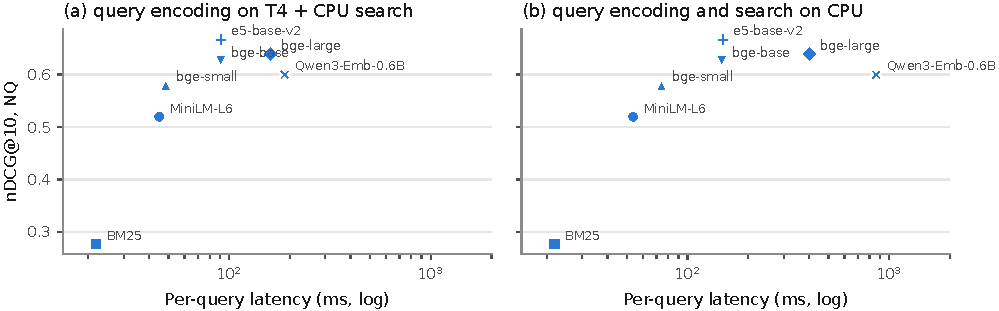
\includegraphics[width=\linewidth]{figs/fig12_latency.pdf}
\caption{NQ nDCG@10 against per-query latency (Phase~1 batch-1 medians, log scale): (a) query encoding on the T4 and exact search on the CPU; (b) both on the CPU.}
\label{fig:latency}
\end{figure}


\end{document}
